\chapter{Registration of Large Models} \label{ch:large_model}
The subject area of this paper is the registration of scans taken of a large and structurally complex physical objects. In particular the focus is on the registration of long-range scans of the entire building with short-range, high resolution close-up scans of some features of it.

In this chapter, the \gls{icp} algorithm's sensitivity to resolution difference between the scans is analyzed. Then a new approach is developed which attempts to make use of the way points are arranged on scanned object surfaces, in order to improve the registration quality.

\section{Evaluation of registration accuracy}
The output of any registration algorithm that aligns a loose point clouds $Q$ with a fixed point cloud $P$ is a rigid transformation matrix $\matr{\hat{M}}$, or possibly an indication that the algorithm has failed. In the ideal case, which is not reachable in practice, it will be equal to the \emph{true} transformation $\matr{M}$.

In order to evaluate the result, it is useful to have a numerical metric $e(\matr{\hat{M}})$ that indicates the ``accuracy'' of  $\matr{\hat{M}}$, both for the cases when the true transformation is known and when it is unknown. It should be minimal when $\matr{\hat{M}} = \matr{M}$, and it should indicate a spatial distance.

\subsection{Known true transformation} \label{sec:lm_known_ttrans}
When $\matr{M}$ is known, the accuracy is measured by how much $\matr{\hat{M}}$ deviates from $\matr{M}$. The rigid transformation, relative to the true transformation, is given by $\matr{\hat{M}}_{\text{rel}} = \matr{M} \matr{\hat{M}} \matr{M}^{-1}$.

Using $\matr{\hat{M}}_{\text{rel}}$, one can calculate for each point $q \in Q$ the \emph{true} correspondence point $q' = \matr{\hat{M}}_{\text{rel}}^{-1} \, \vec{q}$. It is the position in $P$ that corresponds to $q \in Q$. Unless $P$ and $Q$ have the exact same constellation of points, there is generally no point $p \in P$ that coincides with this $q'$. The knowledge of $\matr{M}$ is used to simulate the existence of $P$ with exactly the same constellation.

As a metric for the accuracy of $\matr{\hat{M}}$, the average of the unsigned distances between $q$ and $q'$ is used:
\begin{equation}
e(\matr{\hat{M}}) = \frac{1}{n} \, \sum_{i=1}^{n} \| q_i - q'_i \|
\end{equation}
This metric will be called the \emph{true error}. It is similar to the ICP point-to-point (mean square error) error metric, just with the real correspondences, and without squaring the terms. Using a point-to-plane or other metric would not be useful because the correspondences are exact.

When $\matr{\hat{M}} = \matr{M}$, the absolute minimum $e(\matr{\hat{M}}) = 0$ is reached, as all points $q = q'$ coincide. When $\matr{M}$ is only a translation $\vec{t}$, $e(\matr{\hat{M}}) = \| \vec{t} \|$. When a small rotation with center $\vec{0}$ (the origin $Q$) is added, all points $q$ move away from $q'$ in a circular motion. Using trigonometric approximation for small angles, this length of movement is proportional to $\| q, \vec{0}\|$, and not to the squared distance. Hence taking the average of unsigned distances $q - q'$ can give a useful value.

\subsection{Unknown true transformation}
When the true transformation $\matr{M}$ is unknown, no exact metric for the accuracy of the registration can be defined. It is not known for which input value any such error metric $e$ should reach its minimum. Deciding whether the registration is accurate enough ultimately needs some heuristics, such as a human checking whether the point clouds visually appear well enough aligned for their intended purpose.

The point-to-point or other error metrics used by ICP depend on the estimated point correspondences, and attain local minima for values of $\matr{M}$ where the estimated correspondences are incorrect, but the average distance is low. Also the correspondence selection needs to be adjusted in function of the occlusions, different bounds and densities of $P$ and $Q$. An error metric calculated from one-on-one point correspondences is necessarily limited by which points are available in $P$ and $Q$. Techniques such as point-to-plane ICP and generalized ICP try to infer information about the local shape of the surface around a point.

Point-to-point ICP uses a mean squared error, which allows for least squares error minimization. When the goal is just to evaluate the accuracy of a supposed registration, the \emph{mean absolute error} can be more useful. It is the average of the unsigned distances between each point $q$ and its estimated corresponding point in $p$.
\begin{equation}
e(\matr{\hat{M}}) = \frac{1}{n} \, \sum_{i=1}^{n} \| q_i - p_i \|
\end{equation}
This way the error metric approximates the one defined above for the true correspondences.


\subsection{Visualization of error metric} \label{sec:err_vis}
The rigid transformation matrix $\matr{M}$ has $6$ degrees of freedom: three axis of translation and three angles of rotation. Both the translation and the rotation cannot be represented in a continuous way using less than $3$ real numbers. A natural way to map $6$ real numbers to a rigid transformation is to use a fixed orthonormal coordinate system, and use three values as components for the translation vector, and three values as Euler angles for the rotation.

So an error metric $e(\matr{\hat{M}}_{\text{rel}})$ is a function from $\mathbb{R}^6$ to $\mathbb{R}$. For a good error metric it can be expected that $e(\matr{M}) \approx 0$, and the area around $\matr{M}$ is of interest to evaluate the registration accuracy. It cannot be visualized directly as a six-dimensional density plot, so a way to approximate it is to use two- or one-dimensional cross-sections instead.

An easy way to generate a one-dimensional cross section plot is to fix $5$ components and record the values of $e(m)$ as one component varies. But this creates a bias towards the axis of the used coordinate system which is typically irrelevant to the point cloud. A more useful way is to take a random rigid transformation $\matr{M'}$, and gradually interpolate from $\matr{M}$ to $\matr{M'}$.

As shown in section \ref{sec:rot_interp} a linear interpolation between two rigid transformations can be constructed by linearly interpolating the translation vector components, and calculating the \emph{slerp} for the rotational interpolation. Here an interpolation function $i(t, \matr{M'})$ is constructed based on this, with $t \in [-1, +1]$. It is such that $i(-1, \matr{M'}) = \matr{M'}^{-1}$, $i(0, \matr{M'}) = \matr{M}$ and $i(+1, \matr{M'}) = \matr{M'}$.

$\matr{M'}$ is decomposed into the translational part and the rotational part, both are interpolated as described, and then again composed into a rigid transformation. The negative part needs to be handled separately because the slerp is only defined for $t \in [0, 1]$.

For choosing a random rigid transformation, a angular magnitude $\theta$ and translational magnitude $m$ are first fixed. Then two random unit vectors $\vec{t}$ and $\vec{\omega}$ are chosen, according to a uniform probability distribution. The resulting rigid transformation is the composition of the translation $m \vec{t}$, and the rotation around axis $\vec{\omega}$ by angle $\theta$. Both $m$ and $\theta$ can always be taken as positive values, since rotations in the other direction takes place when $\vec{\omega}$ points in the opposite direction. When $\theta = r \, m$ (in radiants), it will move on a sphere of radius $r$ centered at the point cloud origin, by the same amount as it moves on the translation axis. So it makes sense to fix $r$ in function of the size and shape of the model.

Now a visualization of an error metric is created by first choosing $n$ random rigid transformations $\matr{M}_i$, and then plotting $e(i(t, \matr{M}_1)), \cdots, e(i(t, \matr{M}_n))$ against $t \in [-1, +1]$, on the same graph. A similar approach for visualizing error metrics is for instance used by \cite{Boua2013}. An example of a graph generated this way is shown on figure \ref{fig:mea_plot}. It shows the \emph{mean absolute error} error metric measured on a point cloud, with correspondences established using the closest point criterion.

\begin{figure}[h]
\centering
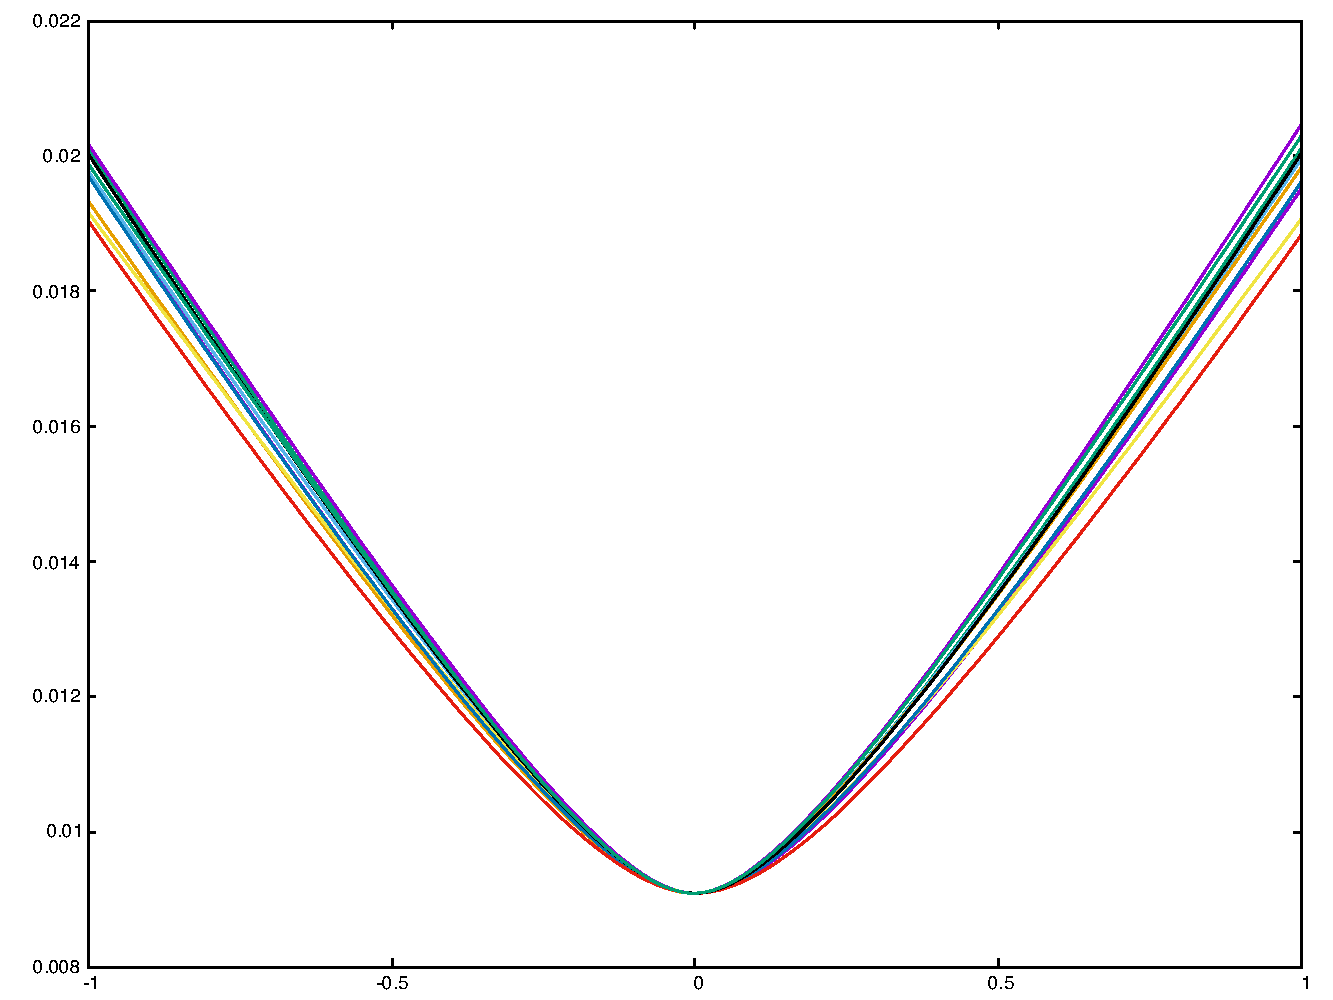
\includegraphics[width=.5\textwidth]{fig/mea_plot.pdf}
\caption{Multi-axis visualization of mean absolute error metric}
\label{fig:mea_plot}
\end{figure}

Because multiple interpolation axis (or planes) cannot easily be visually overlapped, two-dimensional plots of the error function are less useful, unless the two chosen axis have a special significance. For example if they span the plane of an approximatively planar model.


\newpage

\section{Models}
This section describes the point clouds that will be used as input data to test the algorithms.

\subsection{``Hôtel de Ville'' scanning project}
This is a current 3D documentation projection by the the Image research unit of the \emph{Laboratories of Image, Signal processing and Acoustics} (LISA) at ULB. The goal is to create a full 3D model of the ``Hôtel de Ville de Bruxelles'' \footnote{Brussels Town Hall}. It is a medieval building built in the beginning of the 15th century, with a Brabantine Gothic-style architecture.

The data set consists of colorized range image point clouds, including both long range and short range scans. Figure \ref{fig:scan_005} shows one of the long-range scans depicting the front facade. It has a complex shape, and contains stone sculptures and other artwork of which close range scans have been made. The figure shows a reprojection of a colorized point cloud, with the virtual camera position set so as to produce a frontal view of the facade. The scan was taken with the scanner placed on the ground, at the left side near the front gate. As a result, points at higher altitudes, such as on the tower, are less densely distributed. Figure \ref{fig:hdv_033_color} from chapter \ref{ch:theory} also shows one of the long-range scans, taken from the roof of the building.

\begin{figure}[h]
\centering
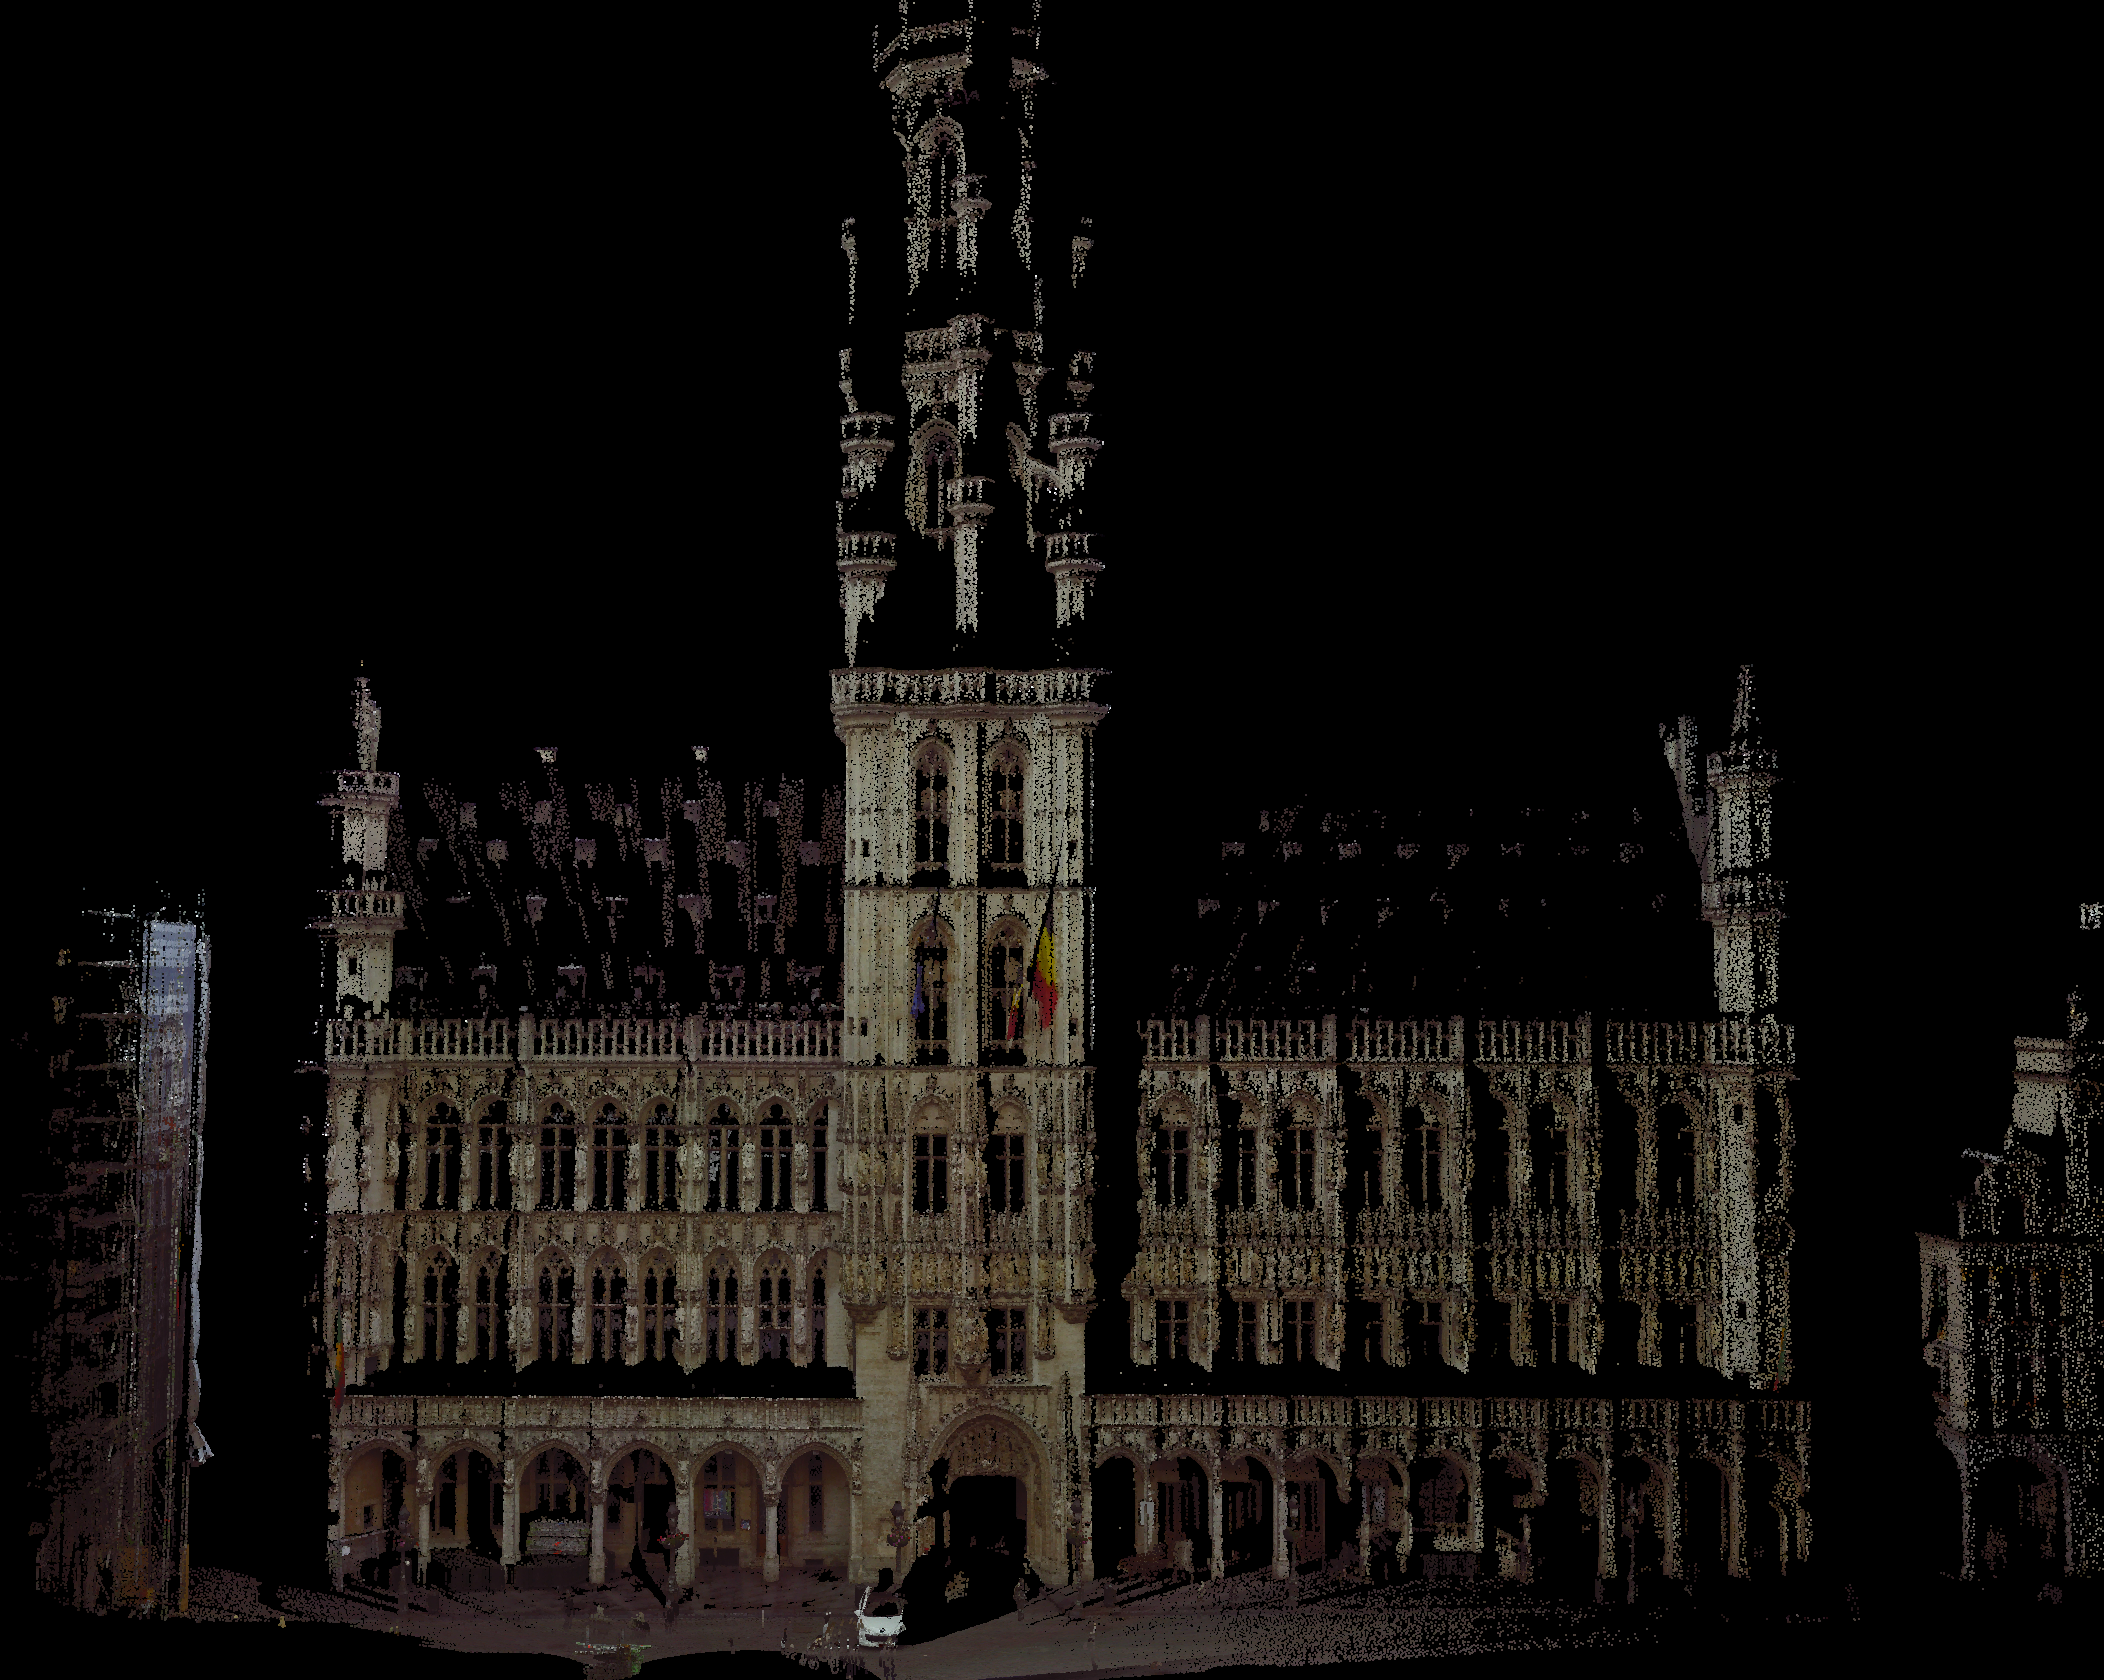
\includegraphics[width=\textwidth]{fig/scan_005.png}
\caption{Depiction of long range scan of Hôtel de Ville facade.}
\label{fig:scan_005}
\end{figure}


\subsection{Dessus-de-porte}
For usage in testing high-to-low resolution registration, scans from the ``dessus-de-porte'', the stone artwork located on top of the front gate of the building, are used. It can be seen from a distance on the long range scan \ref{fig:scan_005}. A much higher resolution, close range scan has also been taken of this part only, and is shown in figure \ref{fig:scan_012}.

\begin{figure}[h]
\centering
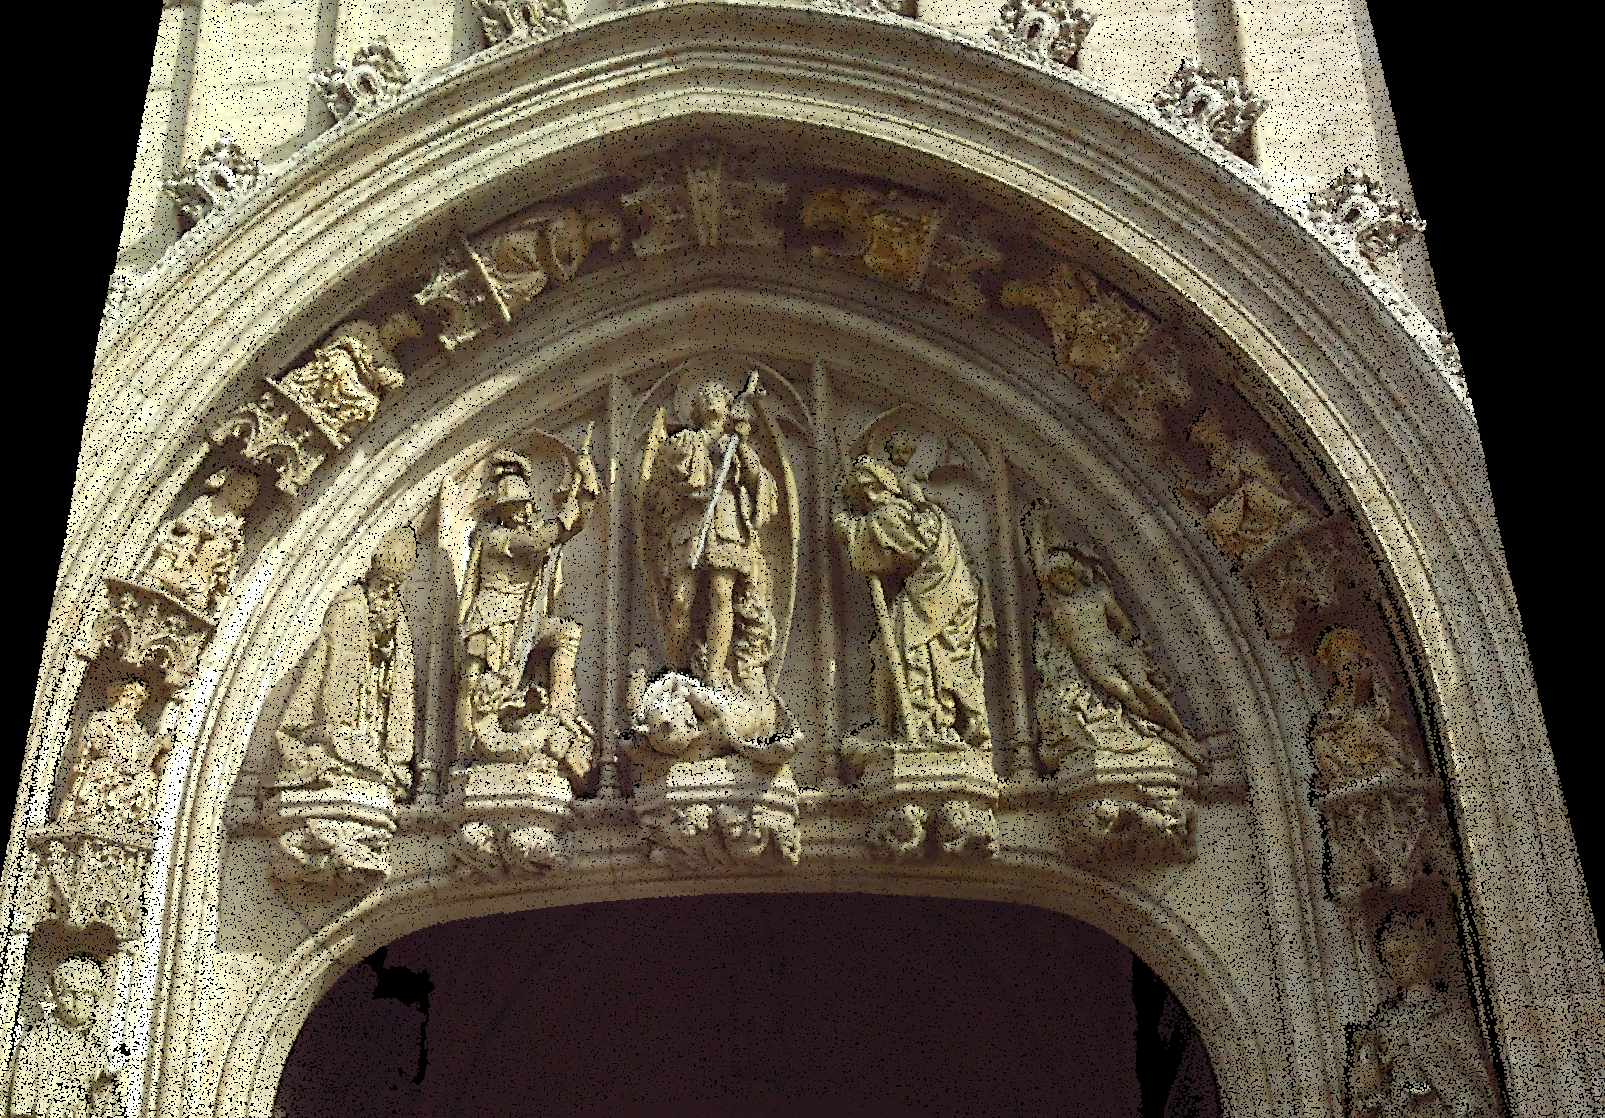
\includegraphics[width=.6\textwidth]{fig/scan_012.png}
\caption{Depiction of short range scan of dessus-de-porte facade.}
\label{fig:scan_012}
\end{figure}

As a 	first step of preprocessing, the same part has been cropped out of both scans, resulting in the two point clouds shown figure \ref{fig:ddp_hilo}:

\begin{figure}[h]
\centering
\begin{subfigure}{.5\textwidth}
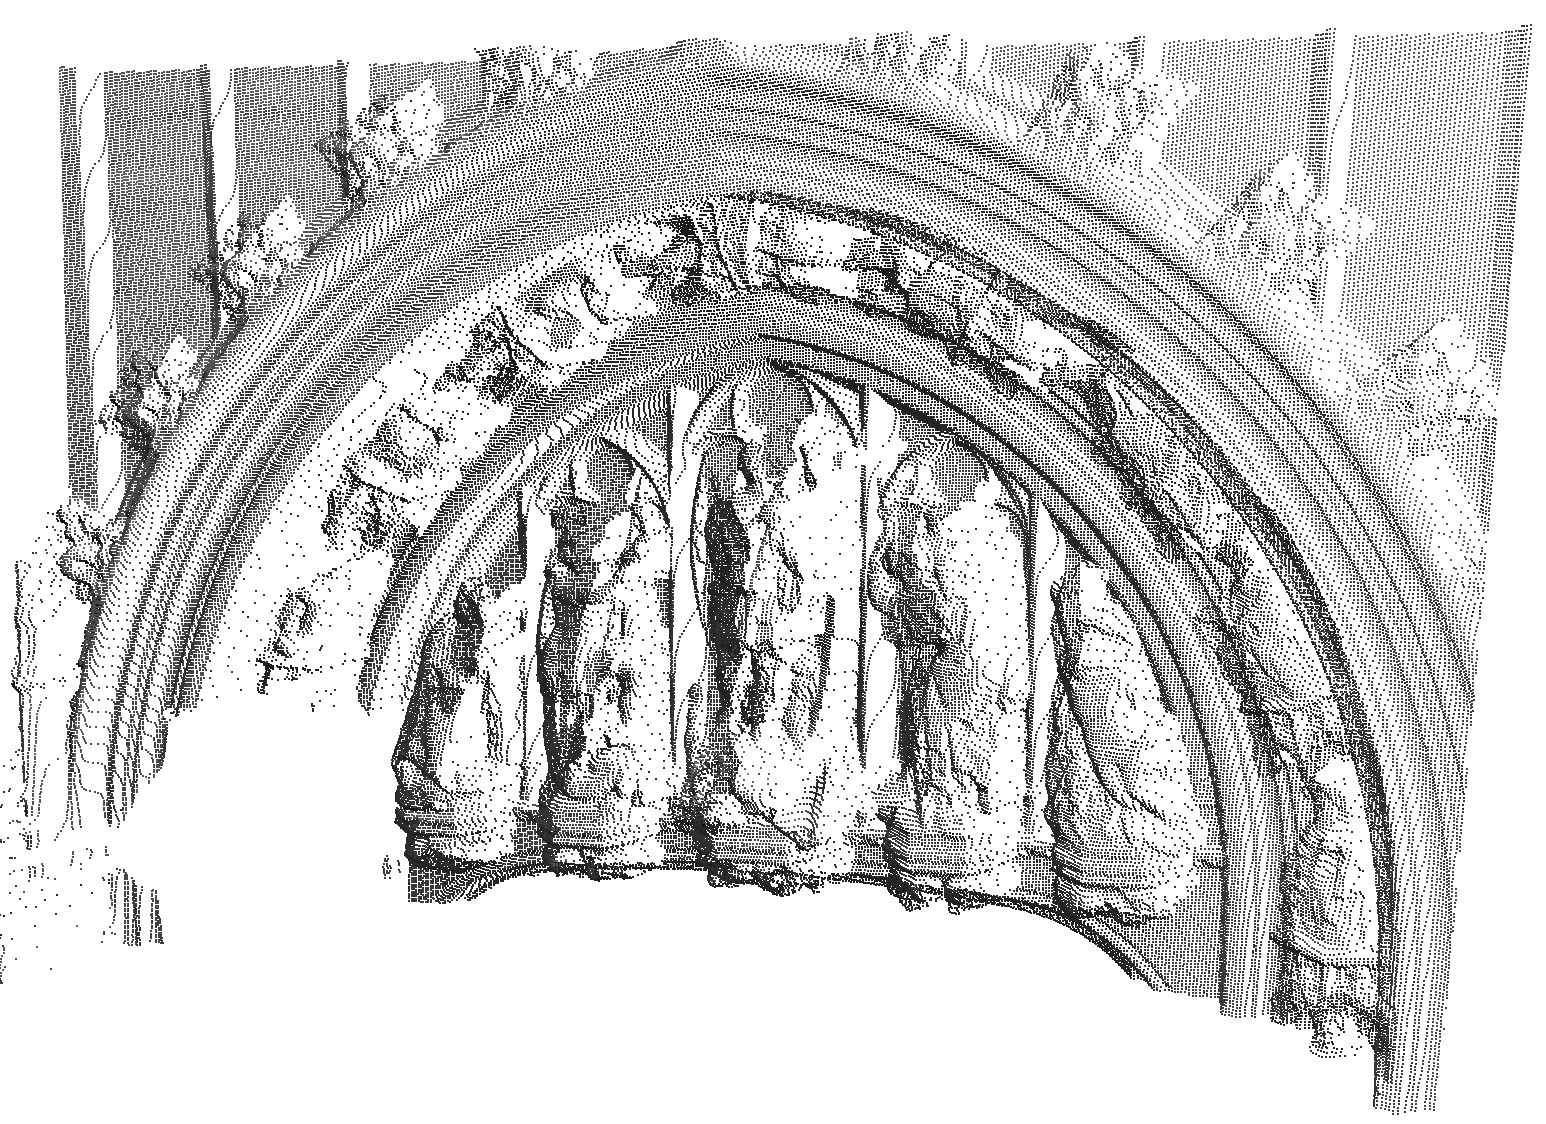
\includegraphics[width=\linewidth]{fig/ddp_LO.png}
\caption{Low-resolution}
\end{subfigure}%
\begin{subfigure}{.5\textwidth}
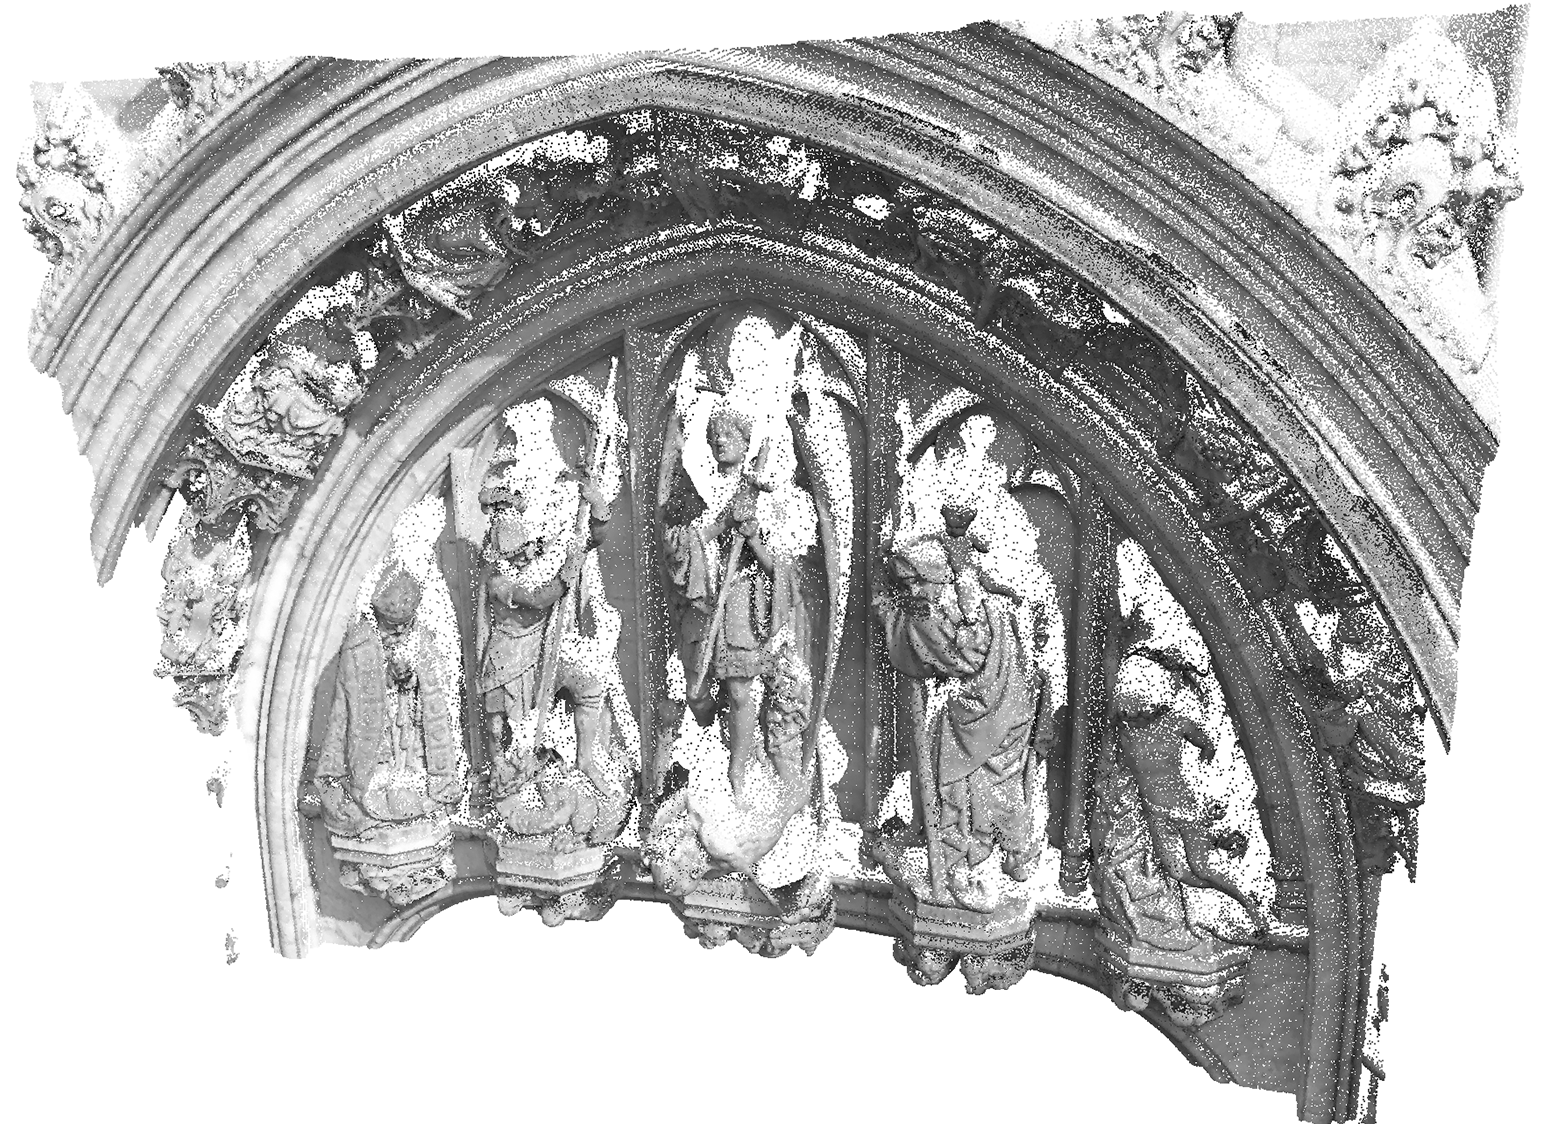
\includegraphics[width=\linewidth]{fig/ddp_HI.png}
\caption{High-resolution}
\end{subfigure}
\caption{Cropped scans of high and low resolution view of dessus-de-porte}
\label{fig:ddp_hilo}
\end{figure}

The colors have been removed on these depictions. The point clouds still have the color information, though it is not be used for registration here. The point clouds also are still \emph{range images}, and information about the relative scanner pose is retained. It can be seen that the low resolution scan has a much lower point density. Its average distance between neighboring points, on flat surfaces facing the scanner, if about $10$ times higher than that of the high resolution scan. The high resolution scan has been randomly downsampled as a side-effect of the visualization software. A close-up view of it is seen on figure \ref{fig:closeup_ddp}, later in this chapter. It can be seen that different sides of the sculptures are occluded in the two scans, because they have been recorded from different view points.

These point clouds have been manually coarsely aligned, and the surface normal vectors have been computed using an external software. A goal will be to finely register them.

\subsection{Relief point cloud} \label{sec:relief}
Many different kinds of objects can be scanned and good approaches for processing and registering them vary depend on many factors. To be able to study registration of point clouds, it is useful to generate artificial points clouds for which exact values of the underlying surface can be computed.

For this purpose an artificial point cloud class called ``relief'' point cloud is described, which has similar properties than the dessus-de-porte. An algorithm was devised to generate relief surfaces, which look as shown on figure \ref{fig:relief_render}.

\begin{figure}[H]
\centering
\begin{subfigure}{.5\textwidth}
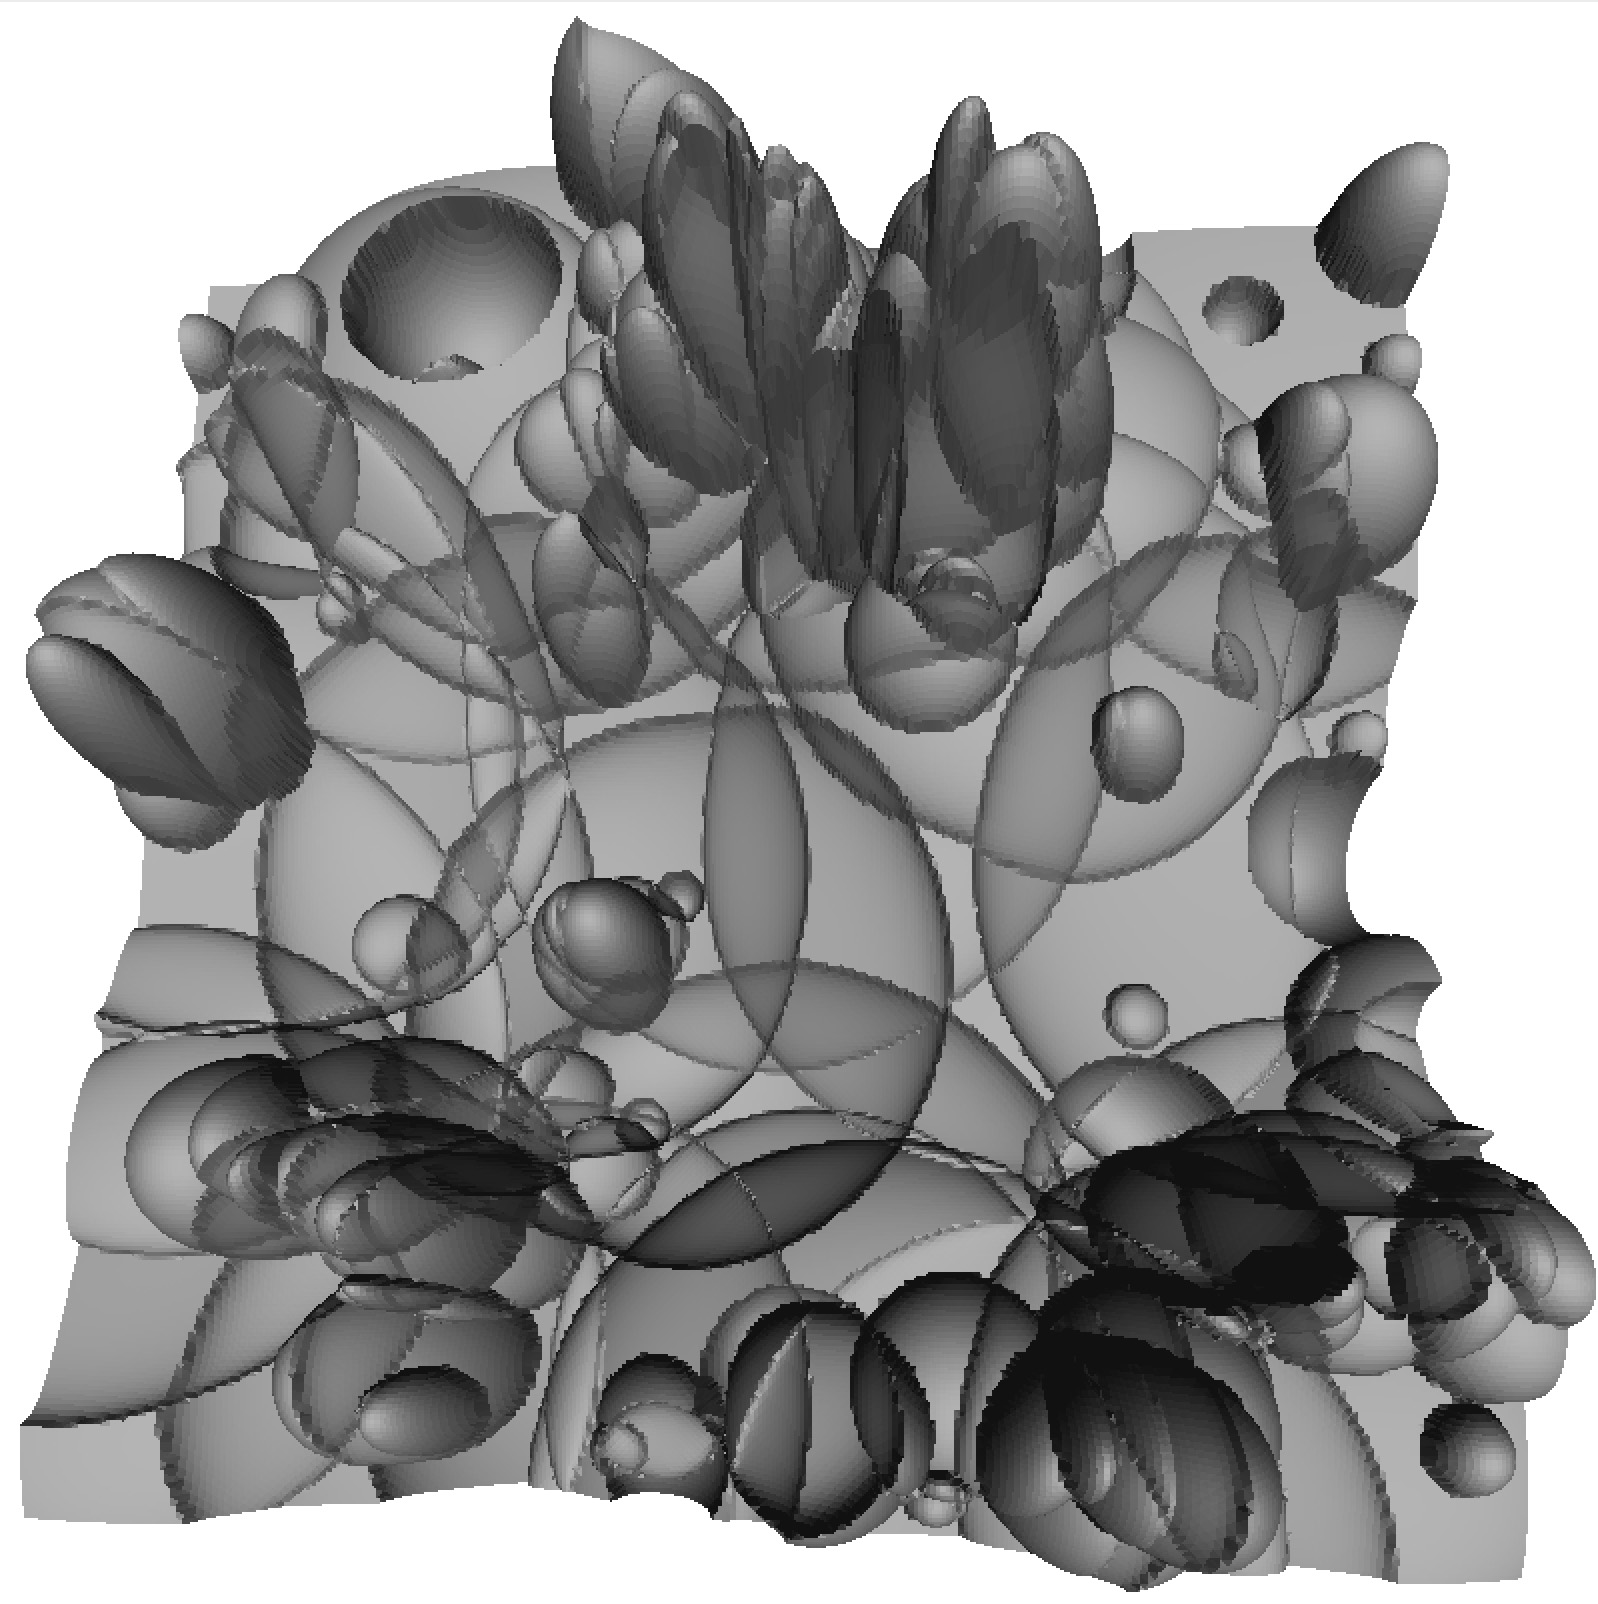
\includegraphics[width=\linewidth]{fig/r1_render2.jpg}
\end{subfigure}%
\begin{subfigure}{.5\textwidth}
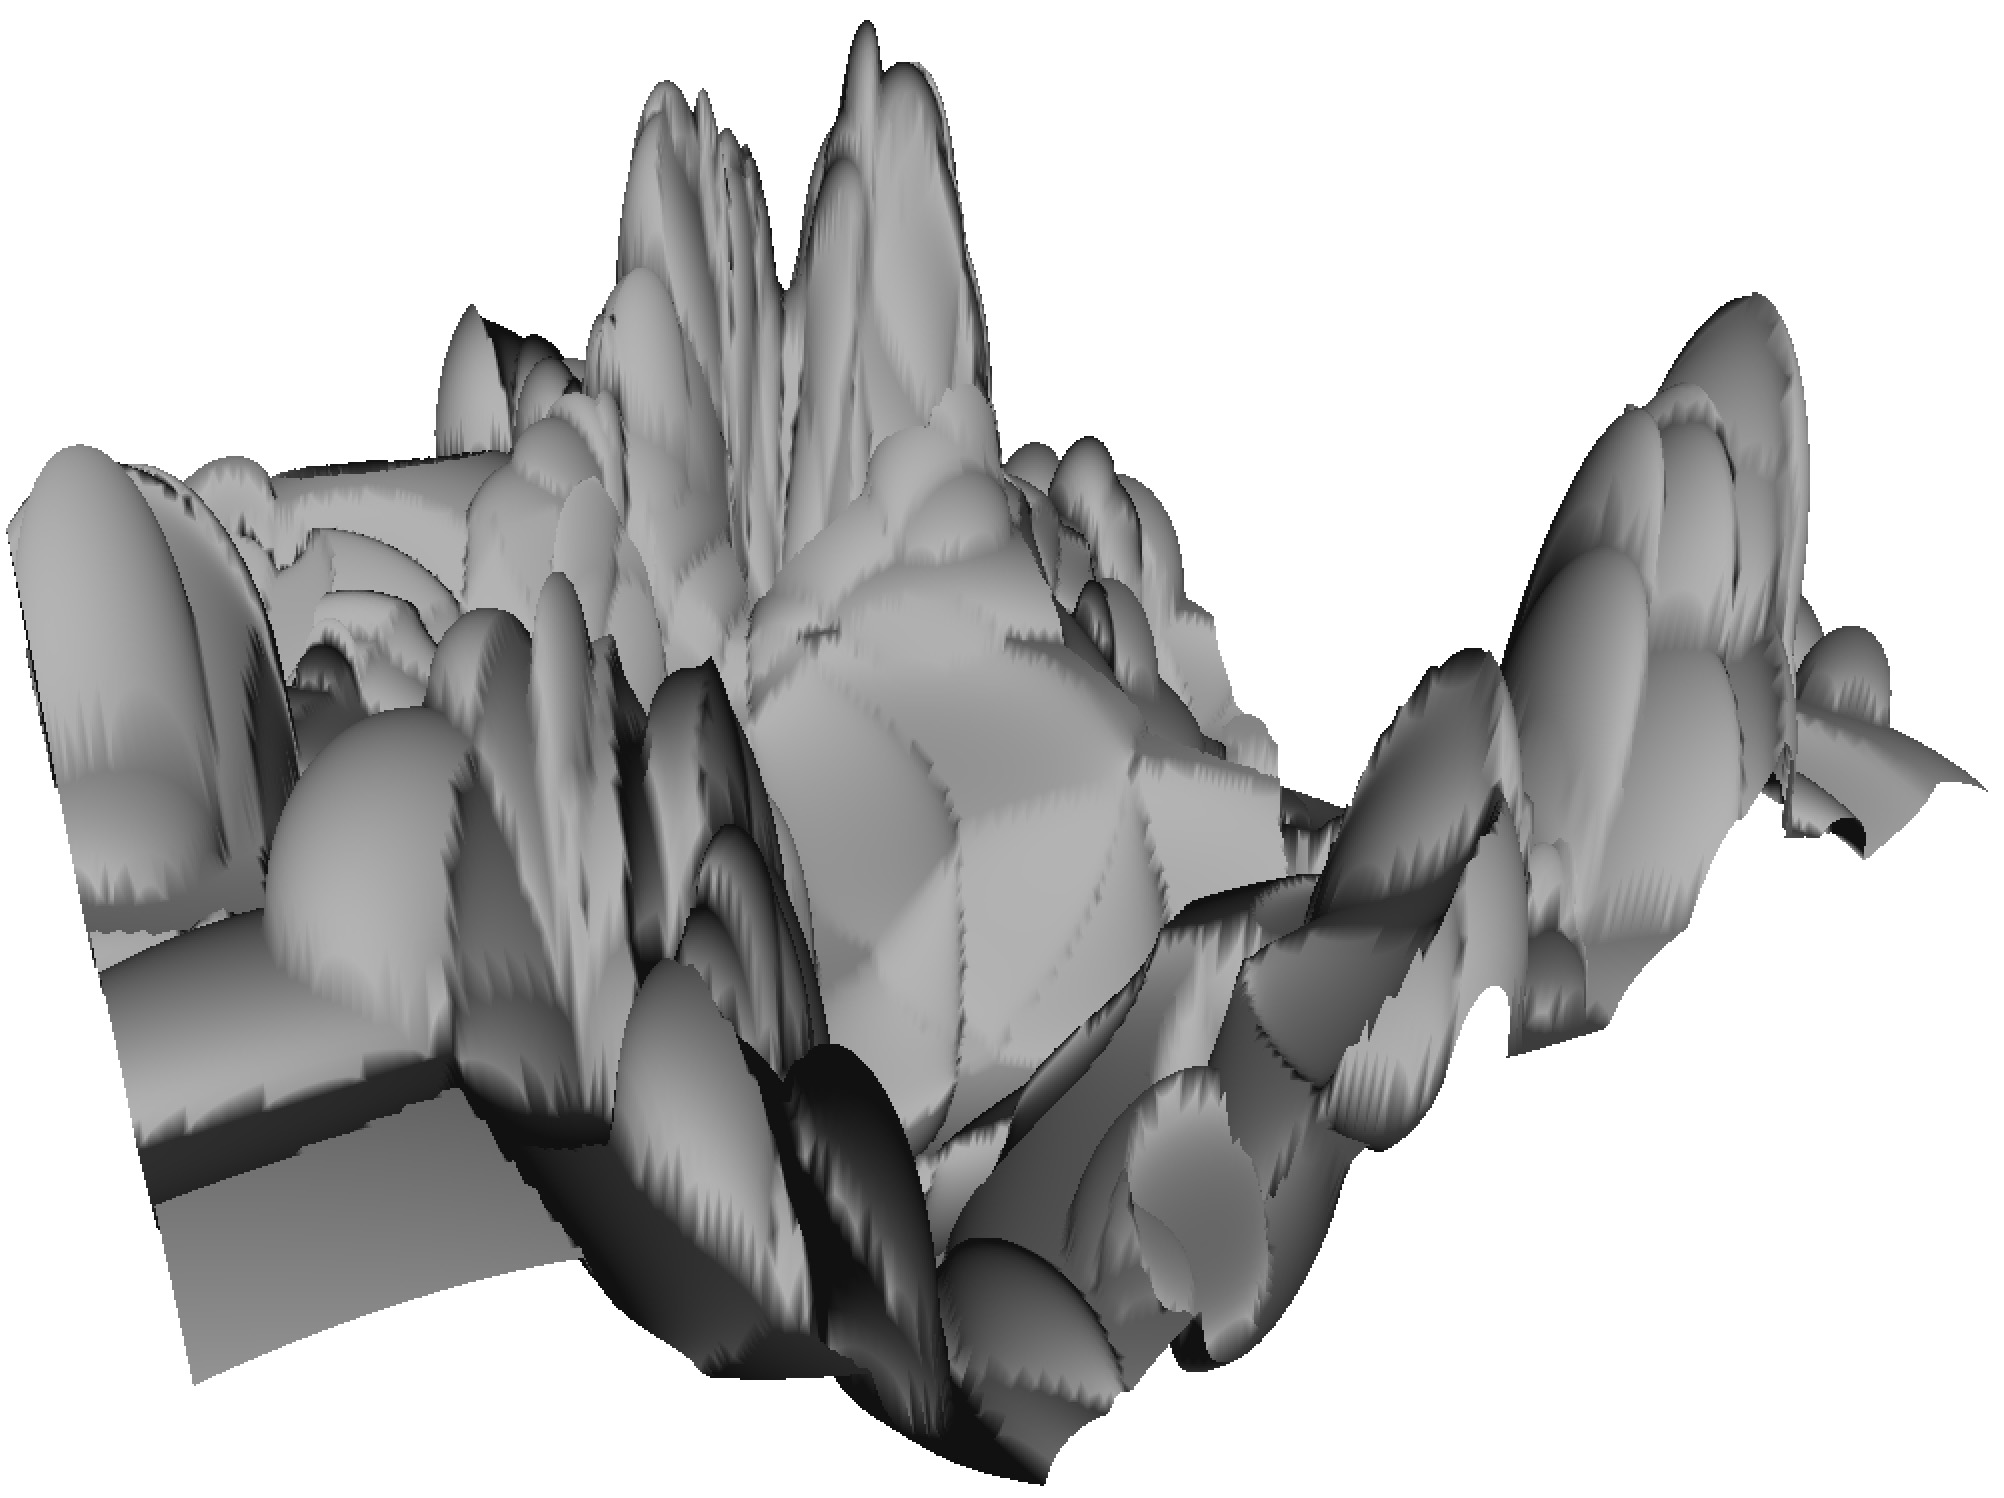
\includegraphics[width=\linewidth]{fig/r1_render1.jpg}
\end{subfigure}
\caption{Artificial relief surface, seen from two view points}
\label{fig:relief_render}
\end{figure}

The entire algorithm is randomized, but can be made deterministic by specifying a seed value for the random number generator. The surface to generate is specified by a \emph{width} $w$, a \emph{height multiplier} $h$, and this seed value.

The generated point cloud is a height map on the XY-plane. Let $z = R[x,y]$ be the $z$ component of the single point with given $x, y$ components. It is defined for $-\frac{w}{2} \leq x,y \leq +\frac{w}{2}$. At first, let $R[x,y] = 0$ for all these points. The result is a square surface of side length $w$.

The algorithm proceeds by pushing randomized ``embossings'' into the surface. The embossings are the shape of a half-sphere distorted in one direction, and is described using the height map formula
\begin{equation}
B_i[x,y] = \pm \, h_i \sqrt{1 - \frac{(x_i - x)^2 + (y_i - y)^2}{r_i^2}}
\end{equation}
A plot of its two-dimensional analogue is shown in figure \ref{fig:relief_B}. $B_i[x,y]$ is set to $0$ for coordinates $x,y$ outside its domain, that is, for $x,y : (x_i - x)^2 + (y_i - y)^2 > r^2$. As a consequence a sharp circular corner is formed around the borders.

A fixed number $n$ of embossings are generated with different parameters, and are added to $R$, so that
\begin{equation}
R[x,y] = \sum_{i=1}{n} B_i[x,y]
\end{equation}

The resulting height map will be split into regions $\{(x,y)\}$ where different subsets of $\{B_i\}$ are active. ($B_i$ is active when $(x,y)$ lies in its domain). $R$ has sharp corners at the border points of all $B_i$. As soon as more than one embossing is active in one region, the $z$ coordinate becomes a sum of square roots, producing a complicated shape for both the continuous surface areas and the corners. Its partial derivatives can still easily be calculated analytically, which allows for accurate computation of normal vectors. 

\begin{figure}[h]
\centering
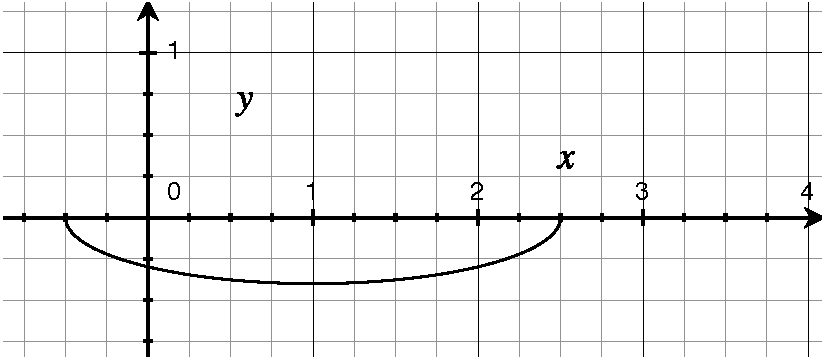
\includegraphics[width=.5\textwidth]{fig/relief_B.pdf}
\caption{2D example for relief embossing, with $h_i = -0.4$, $r_i = 1.5$, and $x_i = 1.0$}
\label{fig:relief_B}
\end{figure}

The radius $r_i$, height $h_i$ and center $(x_i, y_i)$ are randomly chosen for each embossing $B_i$. $x_i, y_i$ are chosen with a uniform distribution in $[-\frac{w}{2}, +\frac{w}{2}]$. The parameters for choosing $r_i$ and $h_i$ are set in such a way that the resulting surface will contain both flat regions and ``spikes'', which occlude parts of the surface when viewed from the side. $h_i$ can be both positive or negative.

\subsubsection{Top-down view point cloud}
Two ways of generating a point cloud of a relief surface are used. The simplest way is to simply take a set of points $\{ x, y, R[x,y] \}$. It results in a \emph{top-down} view of the surface, as seen by an orthogonal projective camera looking in $-z$ direction. From that view point the model has no occluded surfaces. The $x, y$ coordinates are arranged on a square grid. Figure \ref{fig:relief_plain} shows an example of such a point cloud, itself projected with a perspective camera.

\begin{figure}[h]
\centering
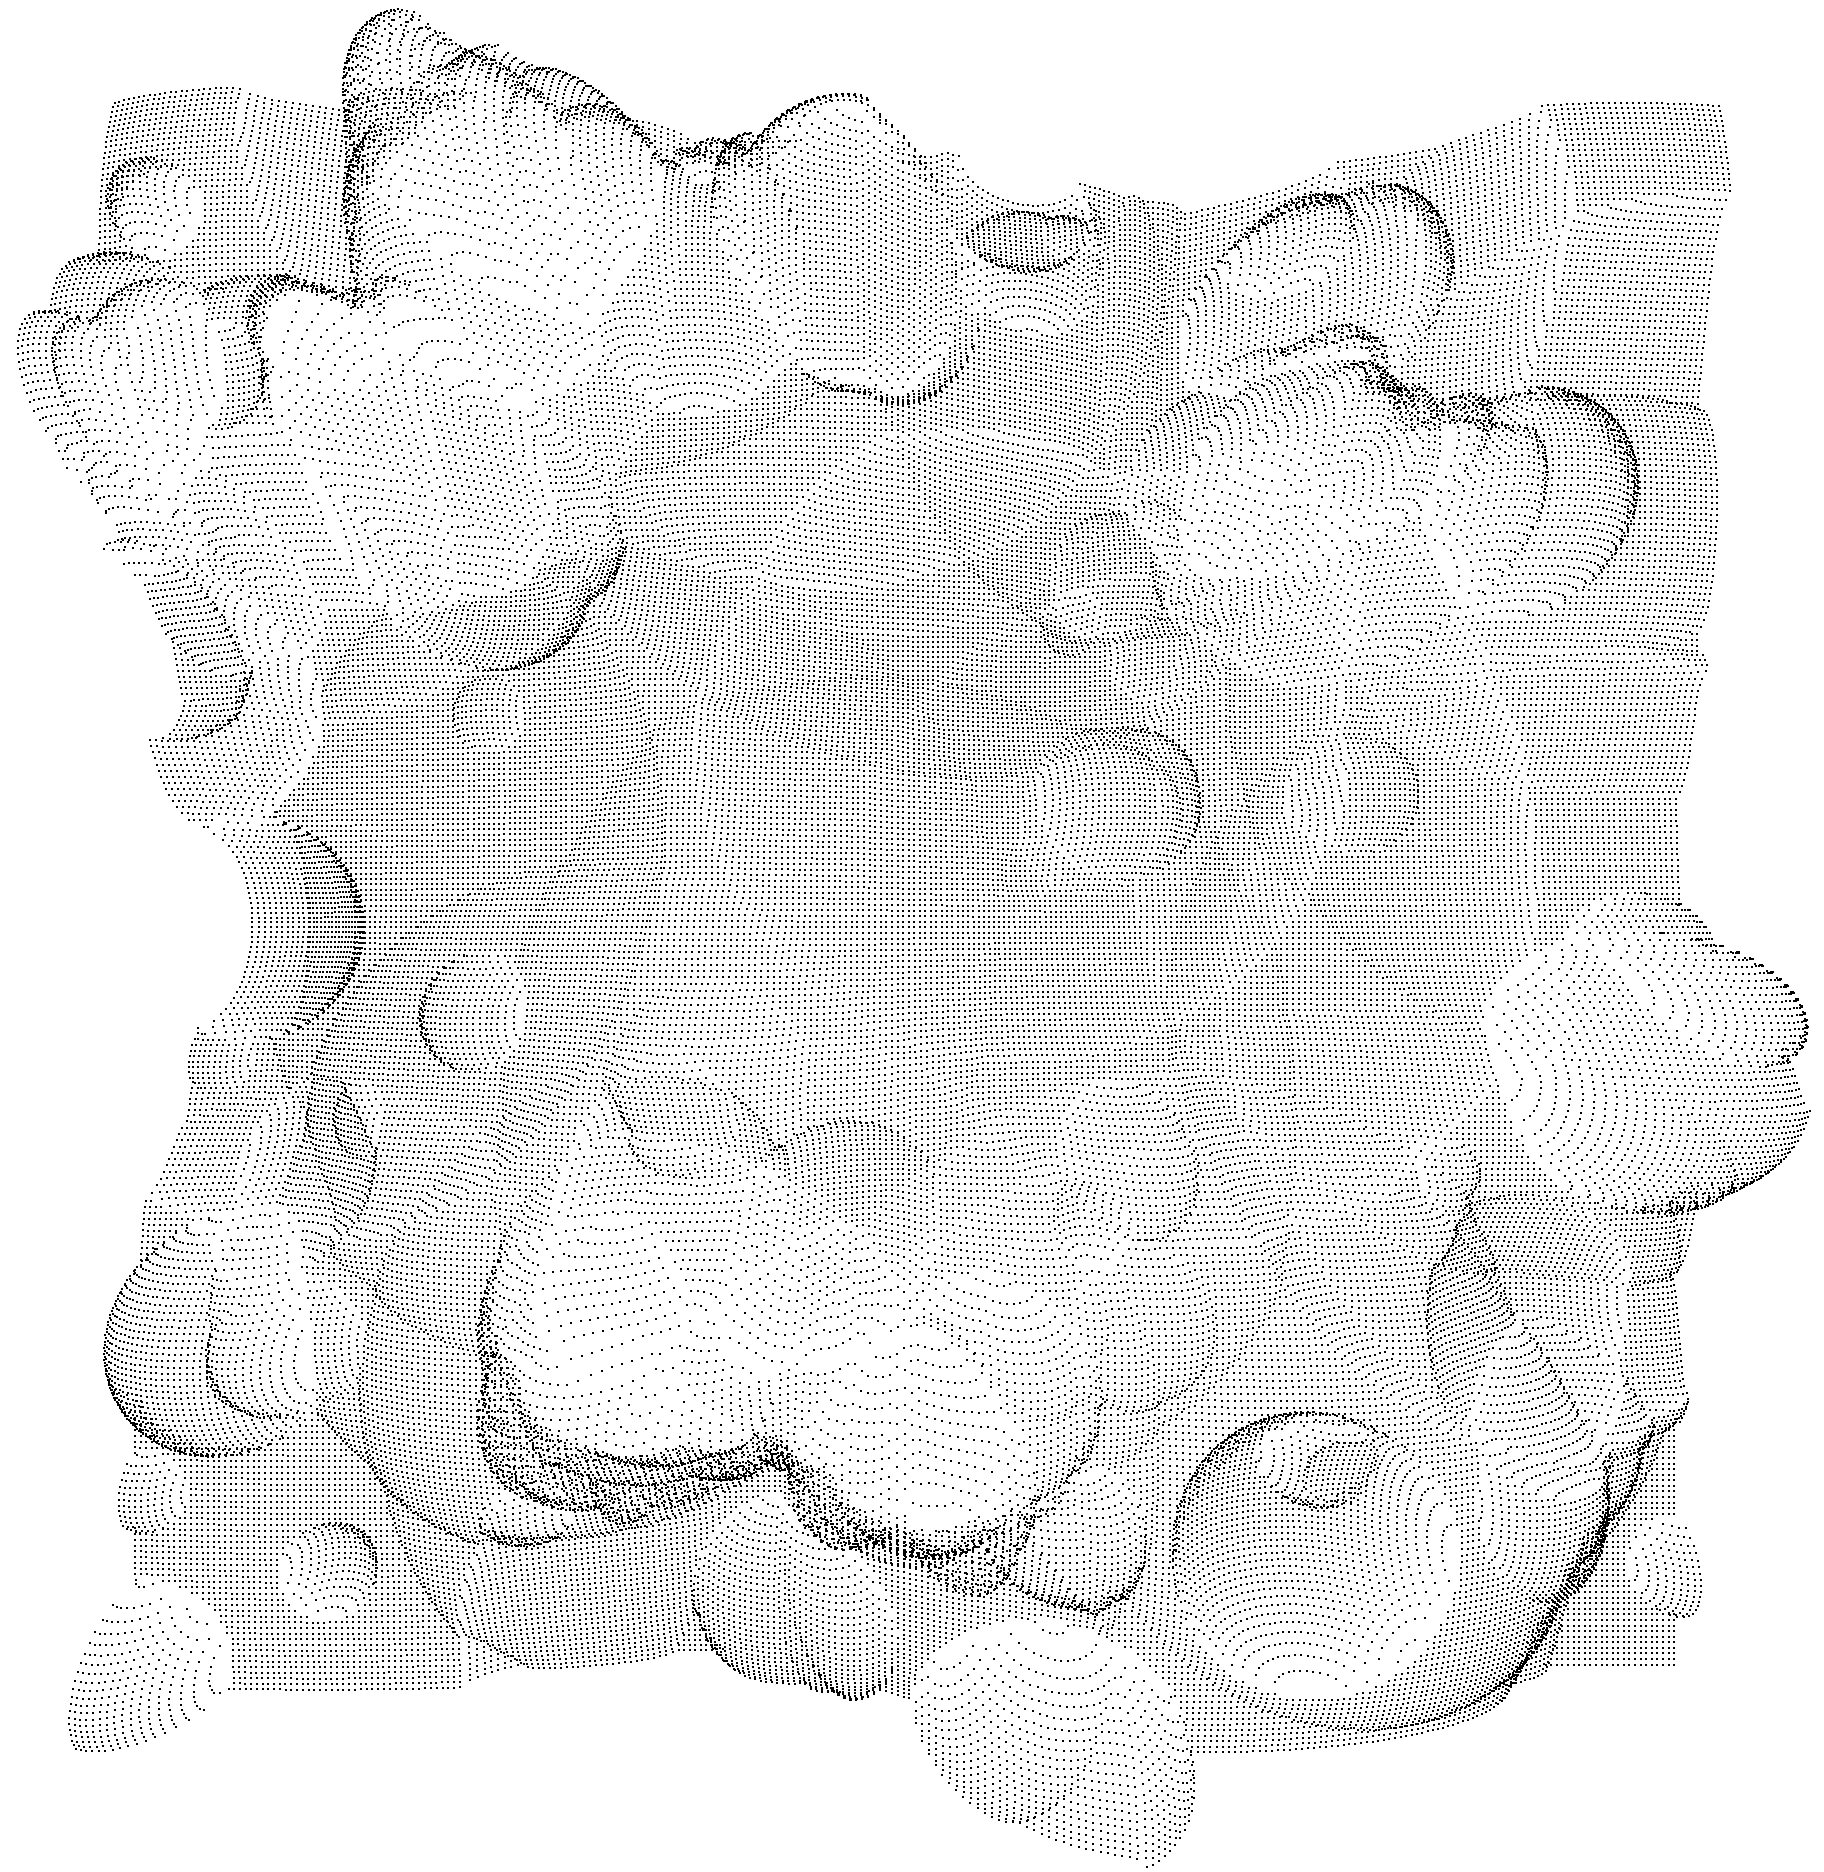
\includegraphics[width=.5\textwidth]{fig/r1_plain.png}
\caption{Top-down point cloud of relief}
\label{fig:relief_plain}
\end{figure}

\subsubsection{Occluded view point cloud}
However the goal of the artificial relief surface was to simulate the kinds of surfaces that occur on real objects, and to get a point cloud with similar properties to a 3D scan of it. So it is important to be able to generate point clouds of the relief as seen from another camera positions, with the occlusions that occur.

A virtual camera is placed near the surface at a given pose, and a range image is generated using it. With an orthogonal projection camera, the point density on the surfaces will remain constant, and with a perspective projection camera, it will decline with distance to the camera.

For the algorithm that creates this range image, a first attempt was to first generate a top-down view point cloud with high enough density, and then project that point cloud into a range image as described in \ref{sec:pc_registration}. However, this inevitably leaves points in the occluded areas.

Another attempt was to implement a ray-tracing method that operates on the expression of $R[x,y]$: For each image pixel, calculate the intersections with the view ray and the surface $R$ and take the closest one. However, these intersections cannot easily be calculated analytically. Firstly, the various regions of $R$ with different active embossings must be considered separately. But even on a single such region, multiple intersection points can still occur, and there is no direct closed-form expression for finding them. So a lot of combinatorics and numerical approximation would be required.

Instead, the implemented algorithm generates a mesh of the surface, projects a depth map of it onto image space, and then back-projects the image pixel coordinates into points. Figure \ref{fig:relief_occlusion} shows the resulting point cloud from two view points, the second one near the projection camera pose.

\begin{figure}[h]
\centering
\begin{subfigure}{.5\textwidth}
	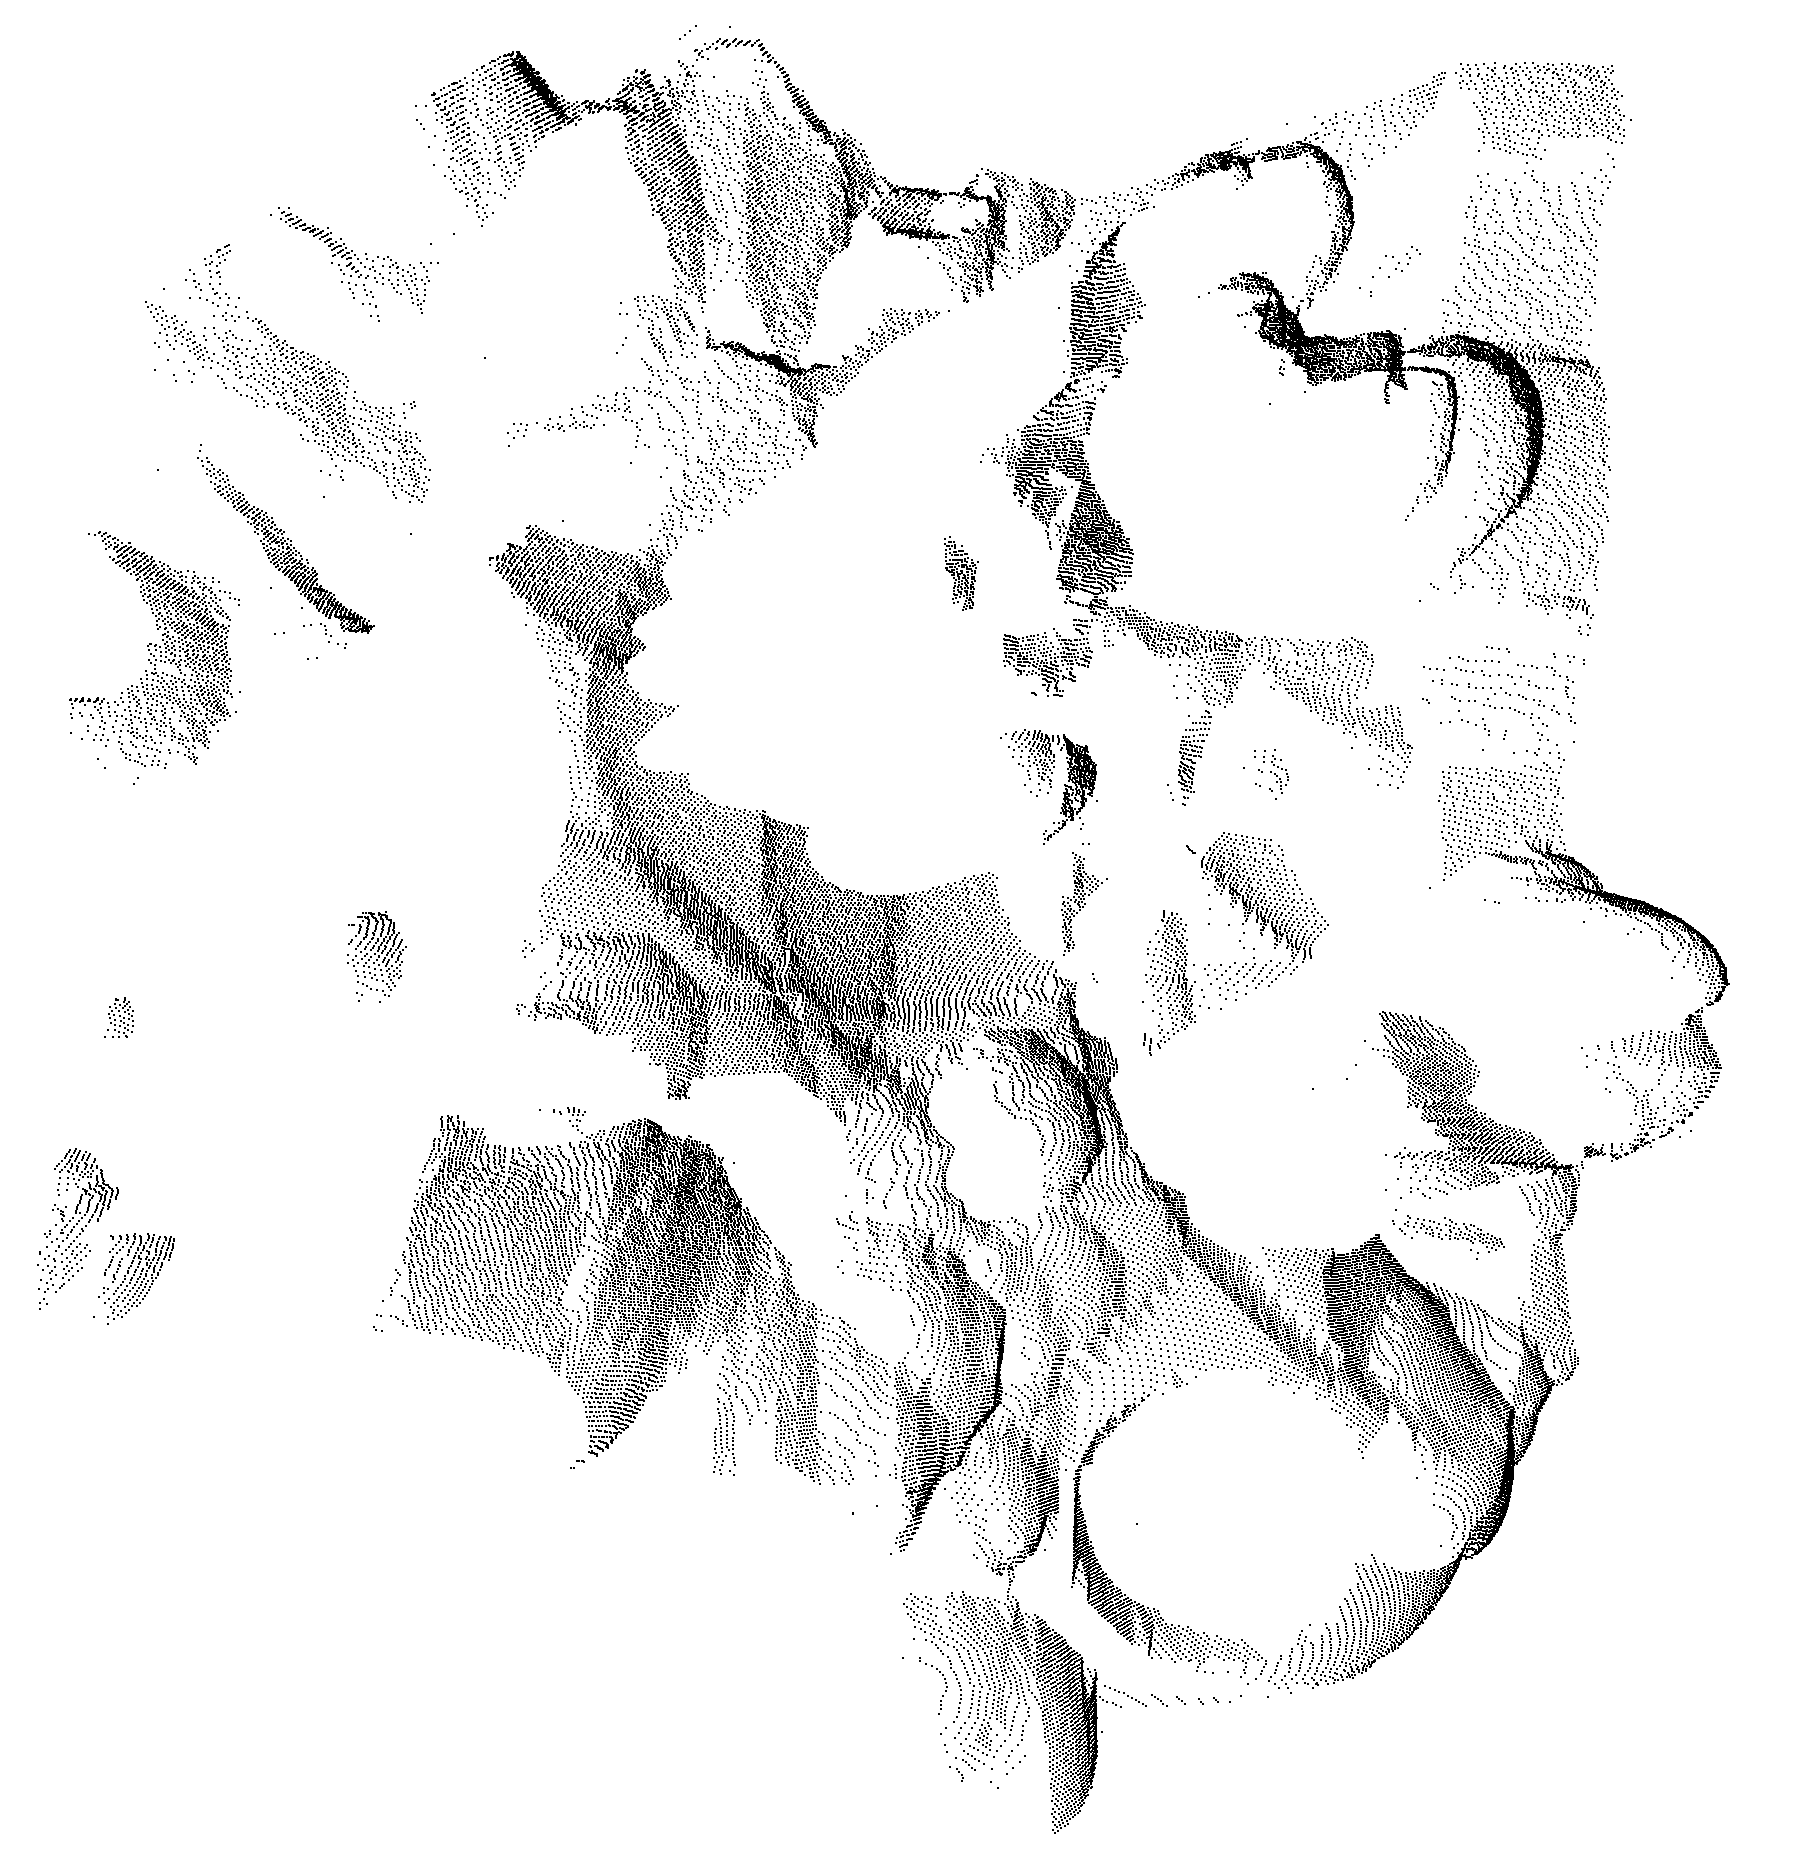
\includegraphics[width=\linewidth]{fig/r1_occlusion.png}
	\caption{Seen from above}
\end{subfigure}%
\begin{subfigure}{.5\textwidth}
	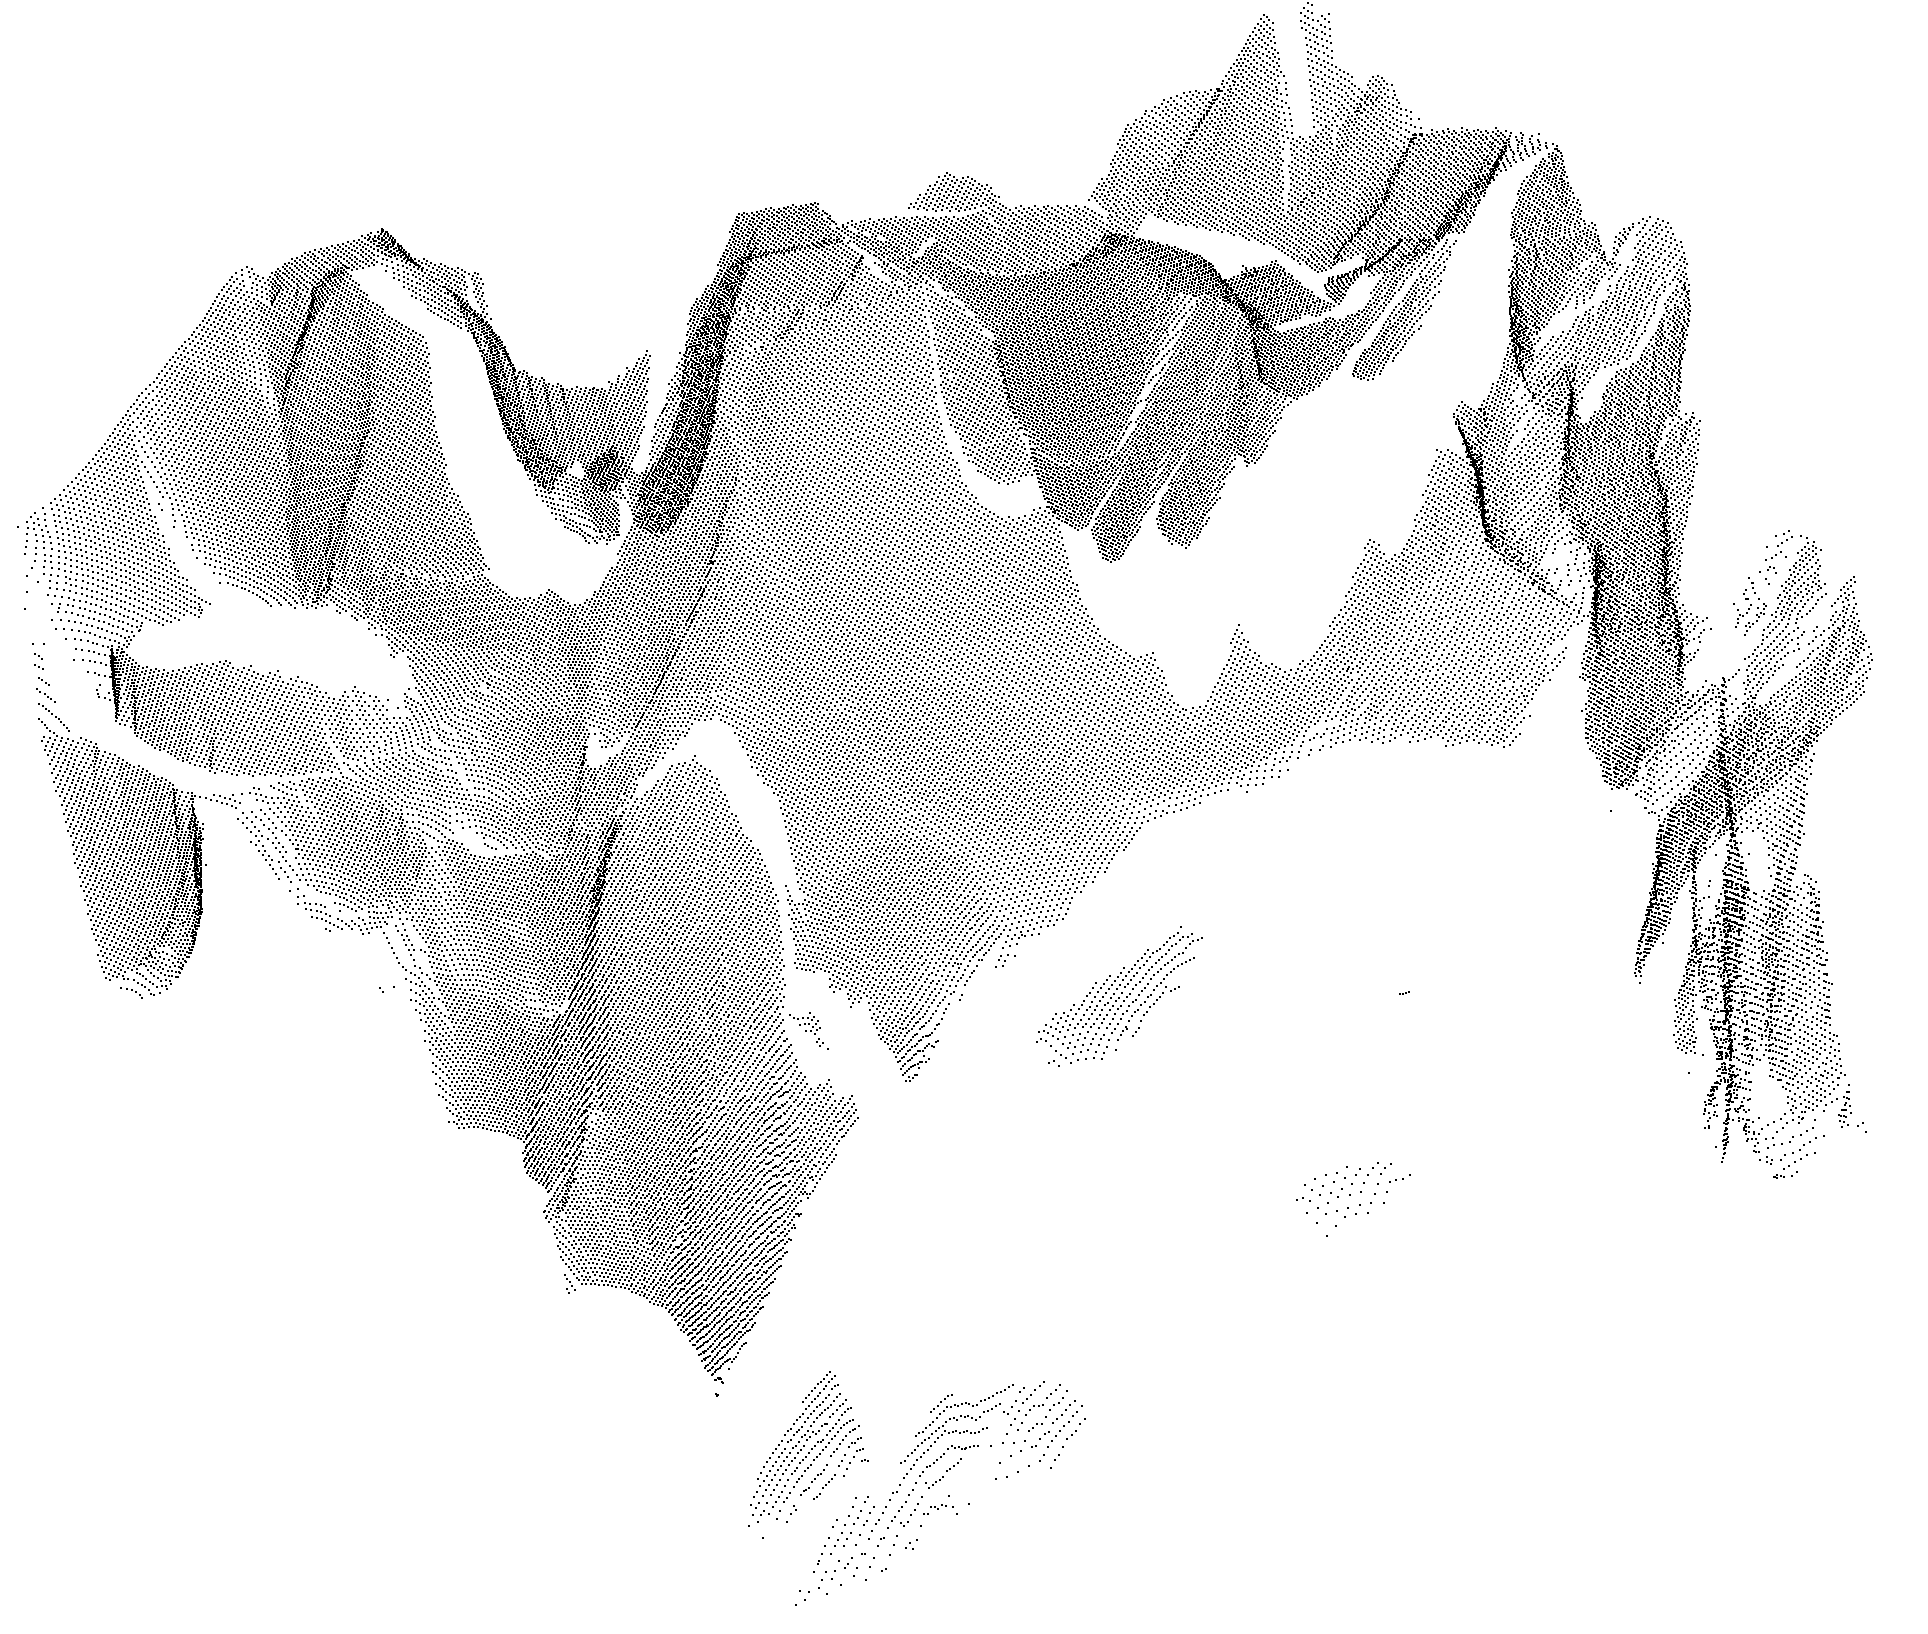
\includegraphics[width=\linewidth]{fig/r1_occlusion2.png}
	\caption{Seen from near the scanner's view point}
\end{subfigure}
\caption{Artificial relief surface point cloud with occlusion}
\label{fig:relief_occlusion}
\end{figure}

A triangle mesh is generated by taking points $\{ x, y, R[x,y] \}$ with the $(x,y)$ coordinates forming a square grid of a given density $\rho$, and adding a diagonal edge into each square, in alternating direction. The number of squares per side must be even for this. As can be seen on the renderings in figure \ref{fig:relief_render}, this mesh does not handle the sharp corners well, but it is sufficient as errors are rectified in a later step.

For each triangle, its three vertices are projected into image space, using the given projection camera. This image is a Z-buffer that contains, for each pixel, the inverted projected depth of the point\footnote{Z coordinate after application of camera projection matrix.}.

The width and height of this image space is set higher than that of the range image by a factor of about $k = 10$. Now each triangle is filled using a 2D rasterization algorithm. For each pixel, the inverted projected depths of the three corner points are linearly interpolated by using barycentric coordinates. This results in the inverted projected depth of the corresponding 3D surface point.

The actual occlusion culling is now done using a depth test: A pixel value is overwritten only if the inverse depth is higher than the previous one. This is the case only if the point is closer to the camera.

Each $k \times k$ square on this image corresponds to a pixel of the final range image. Its center pixel is taken. Given $(x_i, y_i)$ in image space, and the inverse projected depth of the surface point, the 3D coordinates $(x, y, z)$ of the surface points can now be calculated.

Due to the limited accuracy of the mesh, and floating point precision problems, there is some error in this result. It can be rectified by recalculating $z' = R[x, y]$.

\subsubsection{Similarity with dessus-de-porte}
Figure \ref{fig:relief_crop} (called $R$) shows an artificial relief point cloud with occluded view and additionally cropped to a random polygonal region inside the original square. It is superimposed on a top-down point cloud of the same relief.

It is similar to the dessus-de-porte point cloud (called $D$) in these ways:
\begin{itemize}
\item Approximatively planar. For $R$ the plane is the XY-plane, for $D$ it is the stone surface behind the five statues.
\item Seen from a side angle and partially occluded.
\item Contain both smooth surfaces and sharp corners.
\item Some near-planar surfaces, such as non-embossed areas in $R$, and the background stone surface in $D$.
\item Points dispersed on a regular lattice, as a result of the scan-lines, or of the image space in the virtual projection camera.
\end{itemize}

The important difference is that the underlying surface behind $R$ is known. The goal will be to develop a registration method that works for both $R$ and $D$ because of these common characteristics. Using $R$ it can be tested both with and without knowledge of the surface.

\begin{figure}[h]
\centering
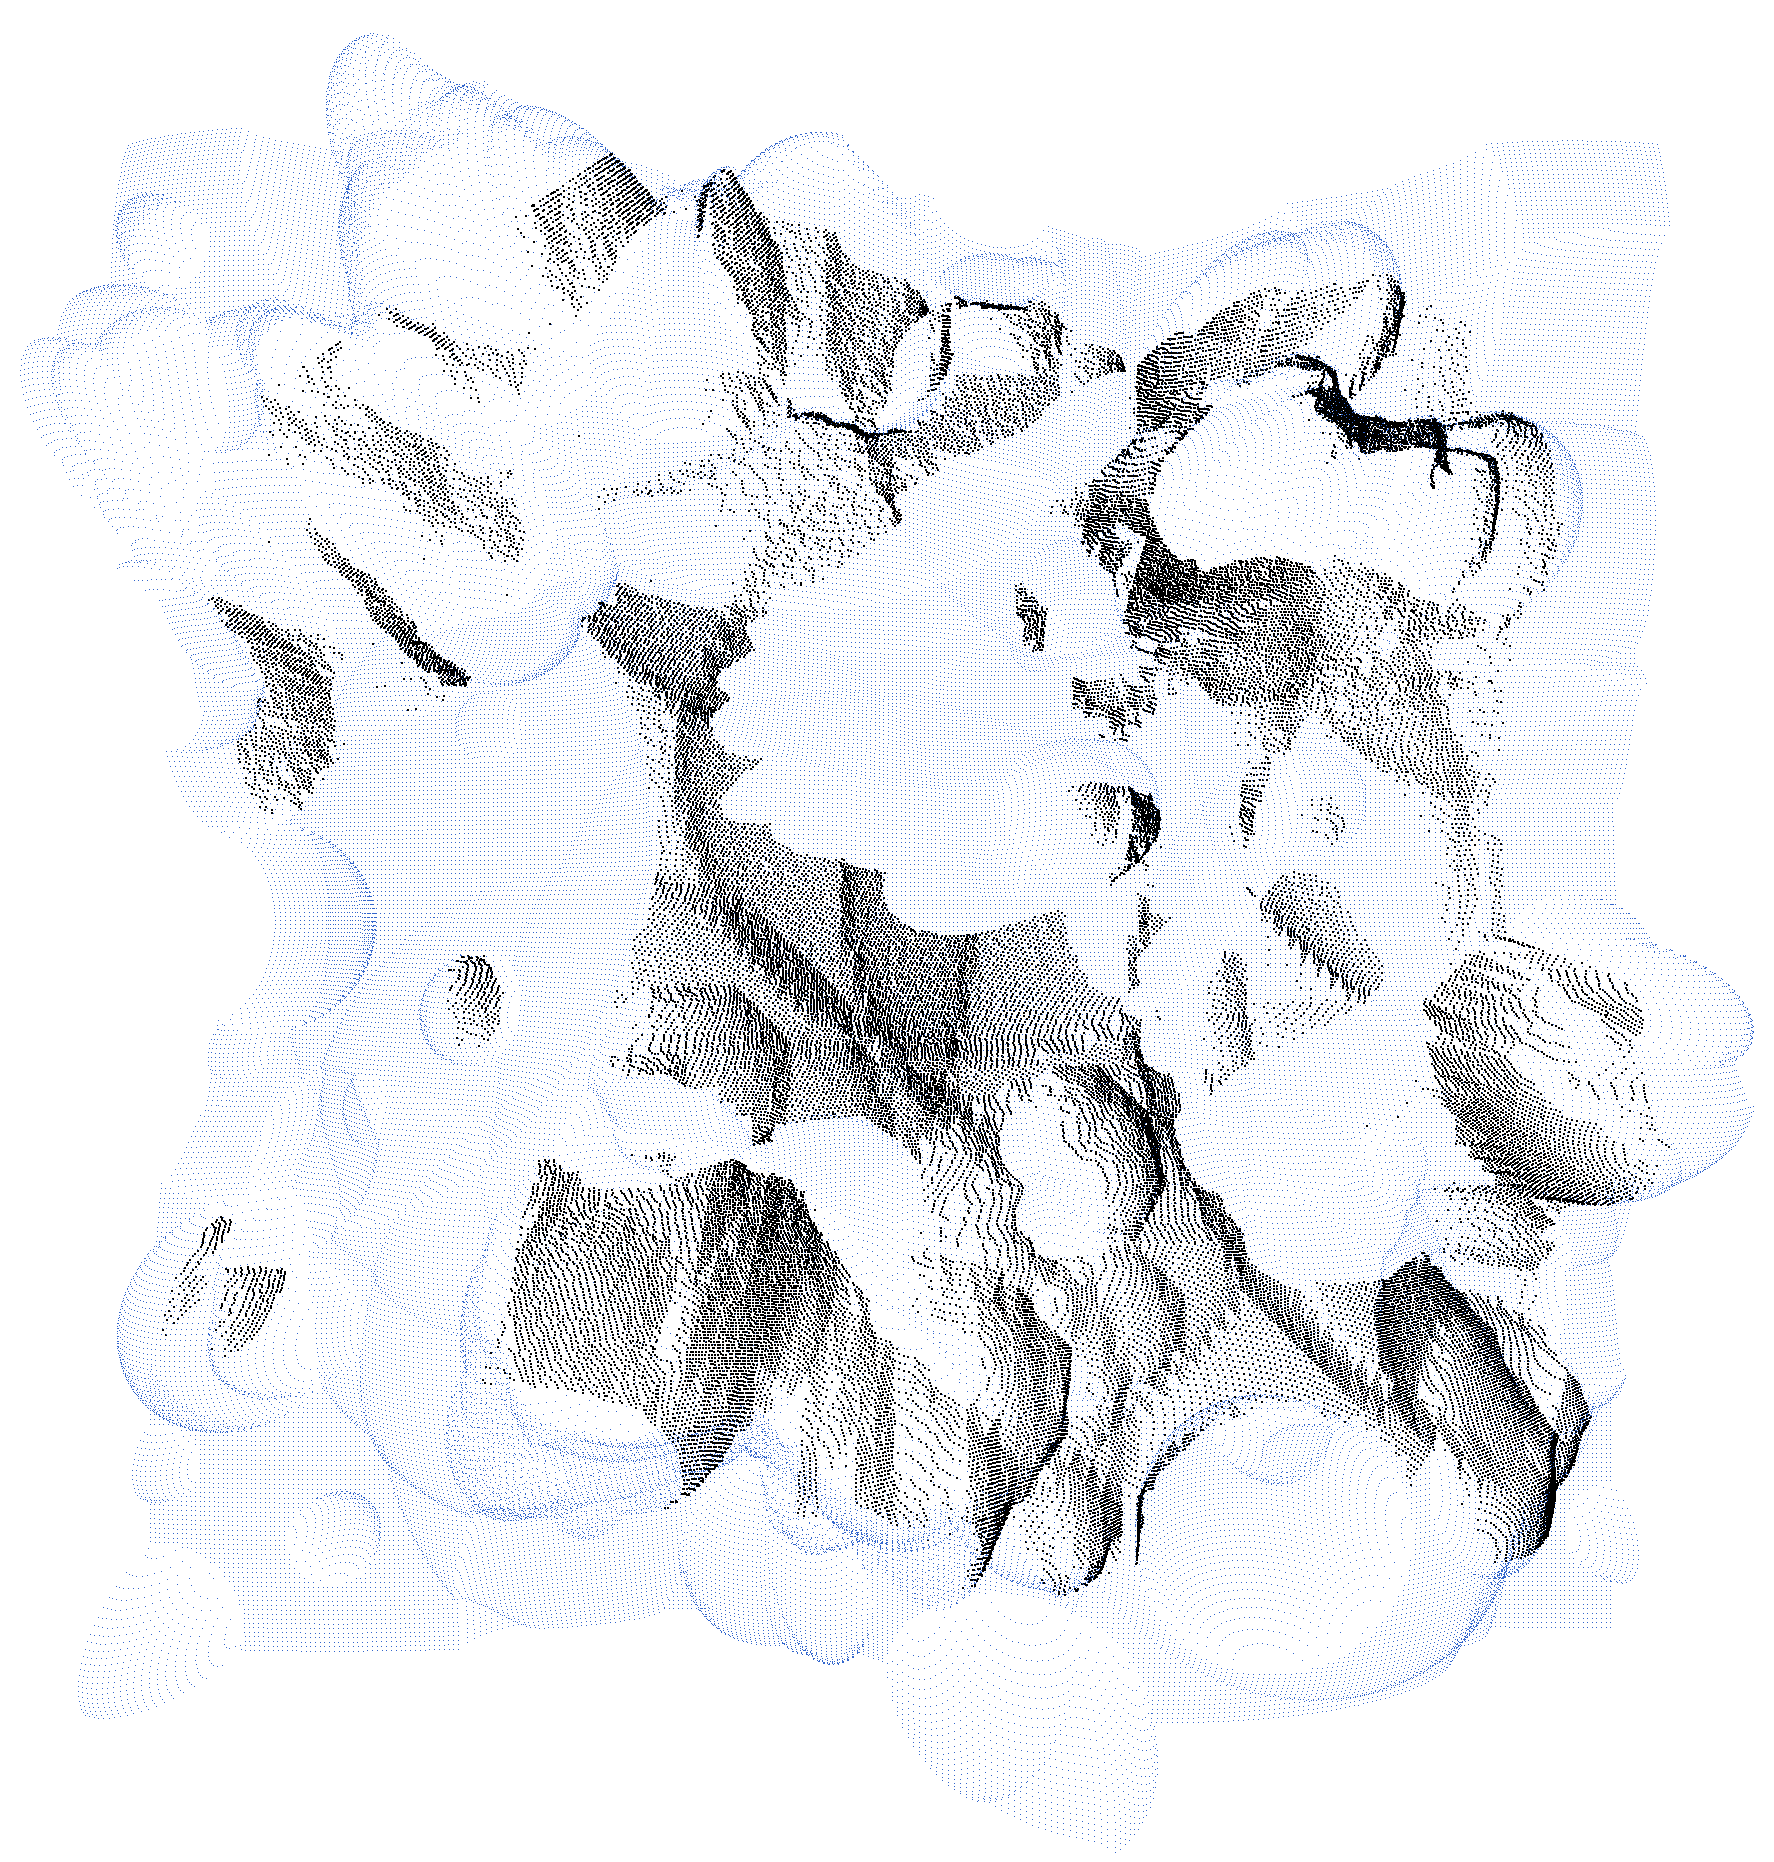
\includegraphics[width=0.7\textwidth]{fig/r1_crop.png}
\caption{$R$: Occluded view point cloud, and top-down point cloud of relief}
\label{fig:relief_crop}
\end{figure}


\subsection{Other models}
For the tests of the ICP algorithm, the well-known \emph{Stanford Bunny} model will also be used. This is a standard 3D test model used in computer graphics, available for free download along with other similar models. It depicts a ceramic figurine of a rabbit and was generated in 1994 at Stanford University. Different versions of it exists, the one used is a point cloud that has already been registered from different view point scans, and covers the entire surface. It consists of $35947$ points.

During this chapter, artificial point clouds consisting of a single plane, or of a sphere, are also used.

\FloatBarrier

\newpage



\section{ICP registration experiments} \label{sec:icp_reg_exp}
Some experiments were run with the \gls{icp} algorithm with different artificial point clouds as input in order to determine how a accurately they can be registered. The true transformation $\matr{M}$ is known, but \gls{icp} only uses the estimated point-to-point error metric using the closest point criterion. After running \gls{icp} on the point clouds, it is tested how closely the final estimated transformation is to $\matr{M}$, that is, how low the \emph{true error} metric of the estimated transformation is.

Because the aim is not to study the convergence evolution of \gls{icp}, but rather the accuracy of the final registration, in most of the test runs the point clouds will be perfectly aligned initially. After registration with \gls{icp} they tend to diverge from this true transformation by a small amount. Two cases are studied: (1) The two point clouds have different resolutions, and (2) They have different camera view poses resulting in low overlap.

For these experiments only the most basic variant of \gls{icp} has been used, with a point-to-point error metric and the closest point criterion. The software framework implemented to conduct the experiments will be described in chapter \ref{ch:implementation}.

\subsection{Different resolutions}
When attempting to register a short-range scan of a relatively small object with the same object in a long-range scan, the short-range point cloud will have a much higher resolution. But fine registration algorithms generally make the assumption that the two point clouds have similar resolutions. The issue of registering point clouds with different resolutions seems to be largely ignored in the literature about point cloud registration algorithms.

A first observation is that in general for \acr{icp}, lowering the resolution of the loose point cloud does not much reduce the accuracy of the registrations. This is shown in experiment \ref{sec:ex_bunny_hilo} (see appendix), in which the Stanford Bunny model is fine registered with a lower density copy of itself. Let $P$ be the fixed point cloud and $Q$ the (downsampled) loose point cloud.

The most basic variant of \acr{icp} is used: All points are selected, correspondences from are taken $Q$ to $P$ by the closest point criterion, no correspondences are rejected, weights are uniform, and the point-to-point error metric is used. The copies are made in such a way that they never have two points in common: $P$ is constructed by taking randomly chosen $50\%$ of the points from the original model, and $Q$ is constructed from the remaining $50\%$. After this $Q$ is randomly downsampled by $60$ different amounts.

The experiment is done in three instances. For the first one (figure \ref{fig:bunny_globmin}), $P$ and $Q$ start out perfectly aligned, and for the two other ones (figures \ref{fig:bunny_globsmall} and \ref{fig:bunny_globmed}), they start out with a small (or larger) random initial transformation. $40$ iterations of the registration algorithm are run and the final errors are recorded.

The plots show the \emph{true error}, as defined in section \ref{sec:lm_known_ttrans}. It is zero if and only if $P$ and $Q$ are perfectly aligned. The X axis indicates the ratio of the number of points $\frac{\|Q\|}{\|P\|}$.


\subsubsection{Analysis}
Two things can be observed: The final error does not depend much on the downsampling level, and the error always converges to about $0.001$, even when $P$ and $Q$ were perfectly aligned to start with.

To define a rigid transformation, three pairs of corresponding points are sufficient as long as the three points do not lie on the same plane. (see section \ref{sec:lsq_align}) So even when $Q$ is reduced to three points the point-to-point error metric can be minimized. \gls{ransac}-based approaches to registration, such as \gls{4pcs} are based on this.

Figure \ref{fig:bunny_hilo_ev} shows how the true error evolves during the $40$ executions of ICP on the first experiment without initial displacement. $P$ and $Q$ were generated to have no common points. When choosing the points closest to the true corresponding point instead, the error does not cancel out completely, and thus the correct alignment is no longer the global minimum of the error metric.

Figure \ref{fig:bunny_first_tcor} shows the state after the registration. $Q$ is rendered in blue color and $P$ in red. From each point $q_i \in Q$ a line segment towards the true corresponding point $q'_i$ is shown, which is not a point $p_i \in P$. On this part $Q$ has deviated towards the right from the correct alignment.

\begin{figure}[p]
\centering
{
	\setlength{\fboxsep}{0pt}%
	\setlength{\fboxrule}{0.5pt}%
	\fbox{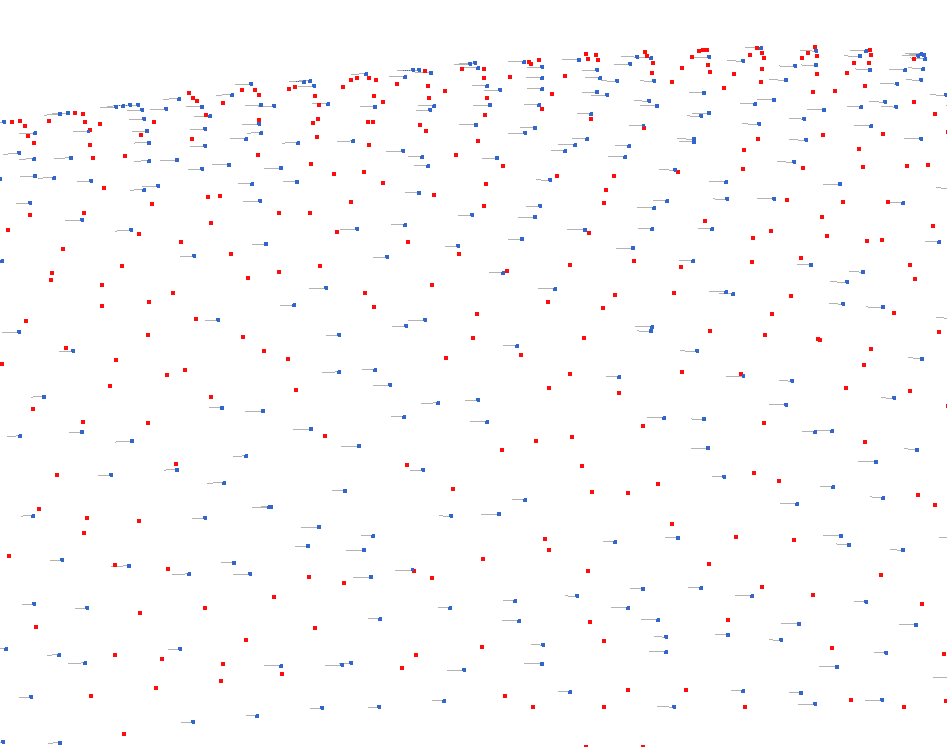
\includegraphics[width=.5\textwidth]{fig/bunny_first_tcor.png}}
}
\caption{Bunny model registered to itself, true correspondences shown}
\label{fig:bunny_first_tcor}
\end{figure}

When $\forall q_i, p_i = q'_i$, the correct alignment would be found. When $P$ and $Q$ are already aligned, $q_i = q'_i$. Figure \ref{fig:bunny_fexp_before} shows the histogram of $\|q'_i - p_i\| = \|q_i - p_i\|$ for the case when $50\%$ (or $80\%$) of the model points are taken for $P$ and the remaining for $Q$, and no additional downsampling is applied.

\begin{figure}[H]
\centering
\begin{subfigure}{.5\textwidth}
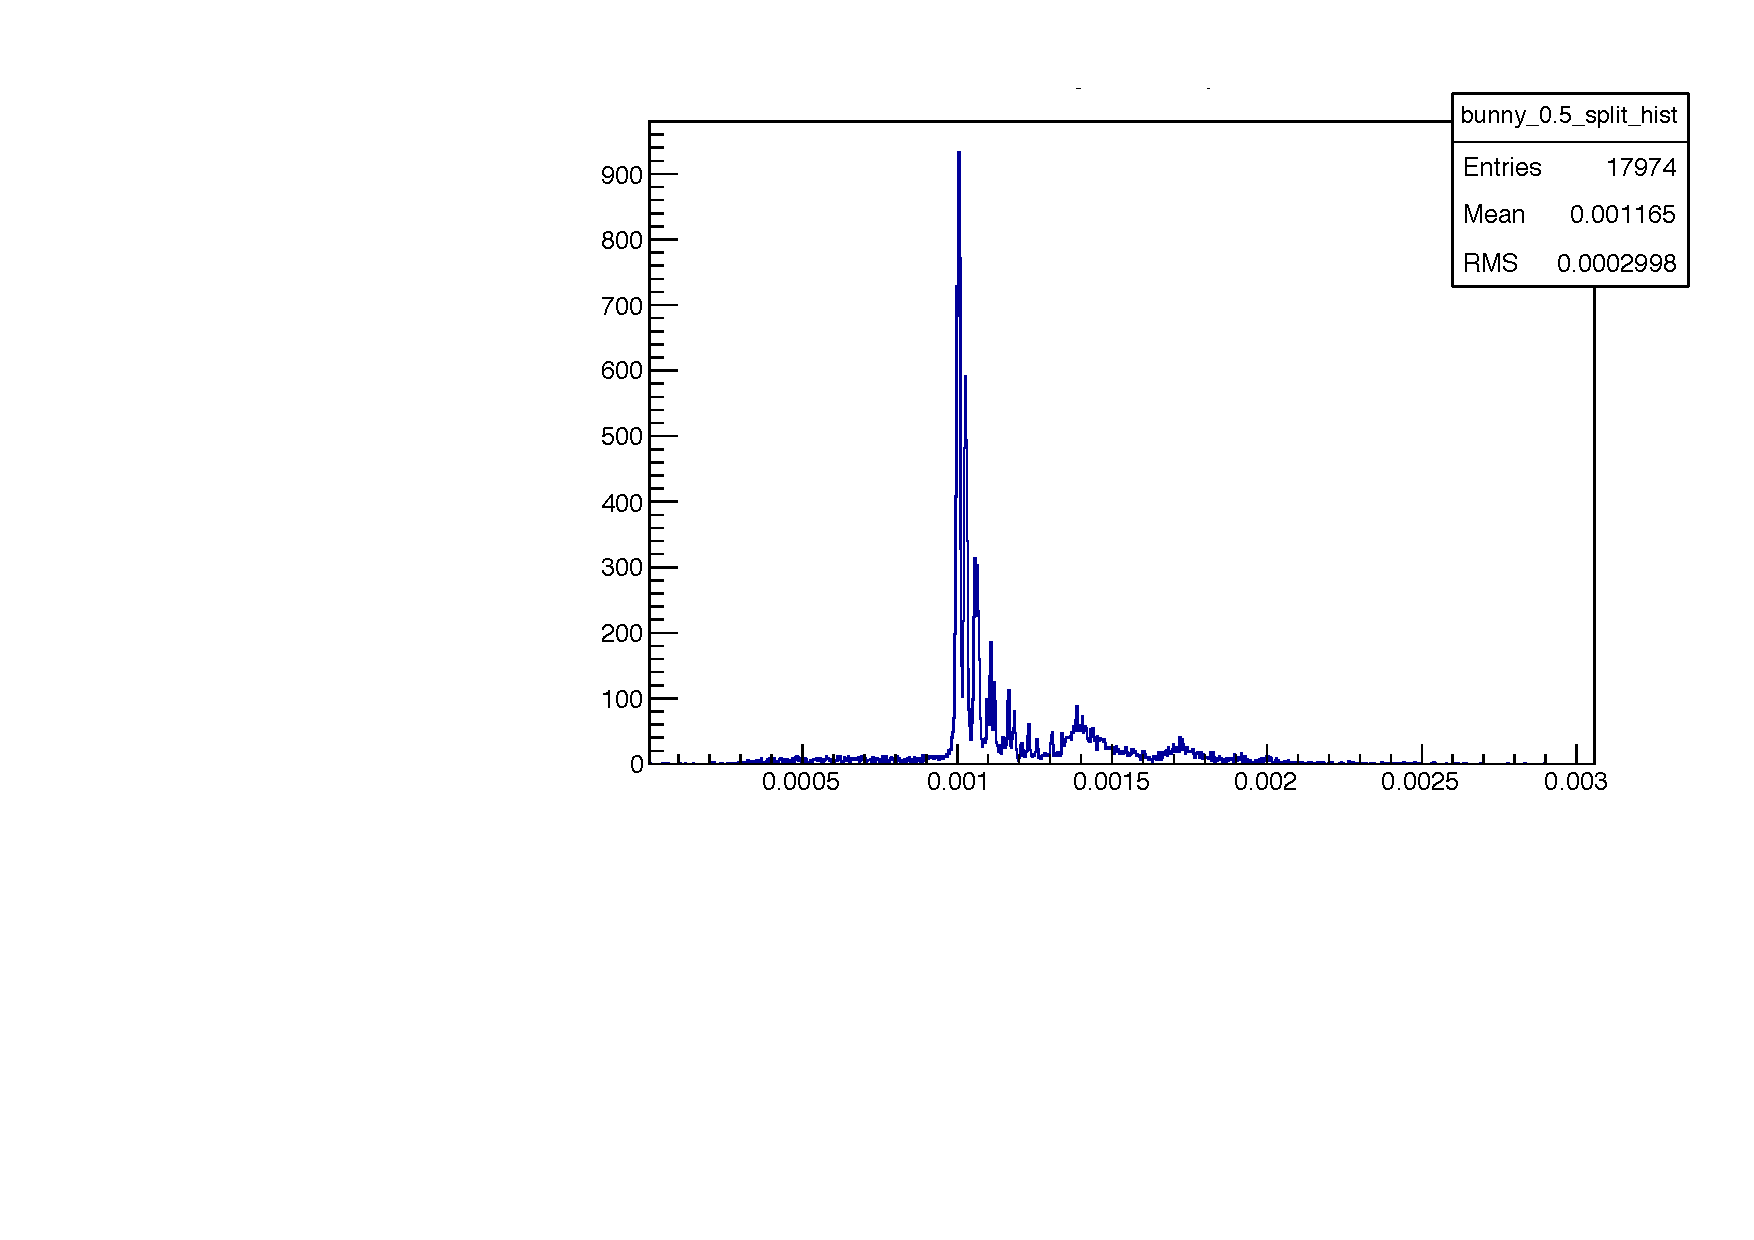
\includegraphics[width=\linewidth]{fig/bunny_05_split.pdf}
\end{subfigure}%
\begin{subfigure}{.5\textwidth}
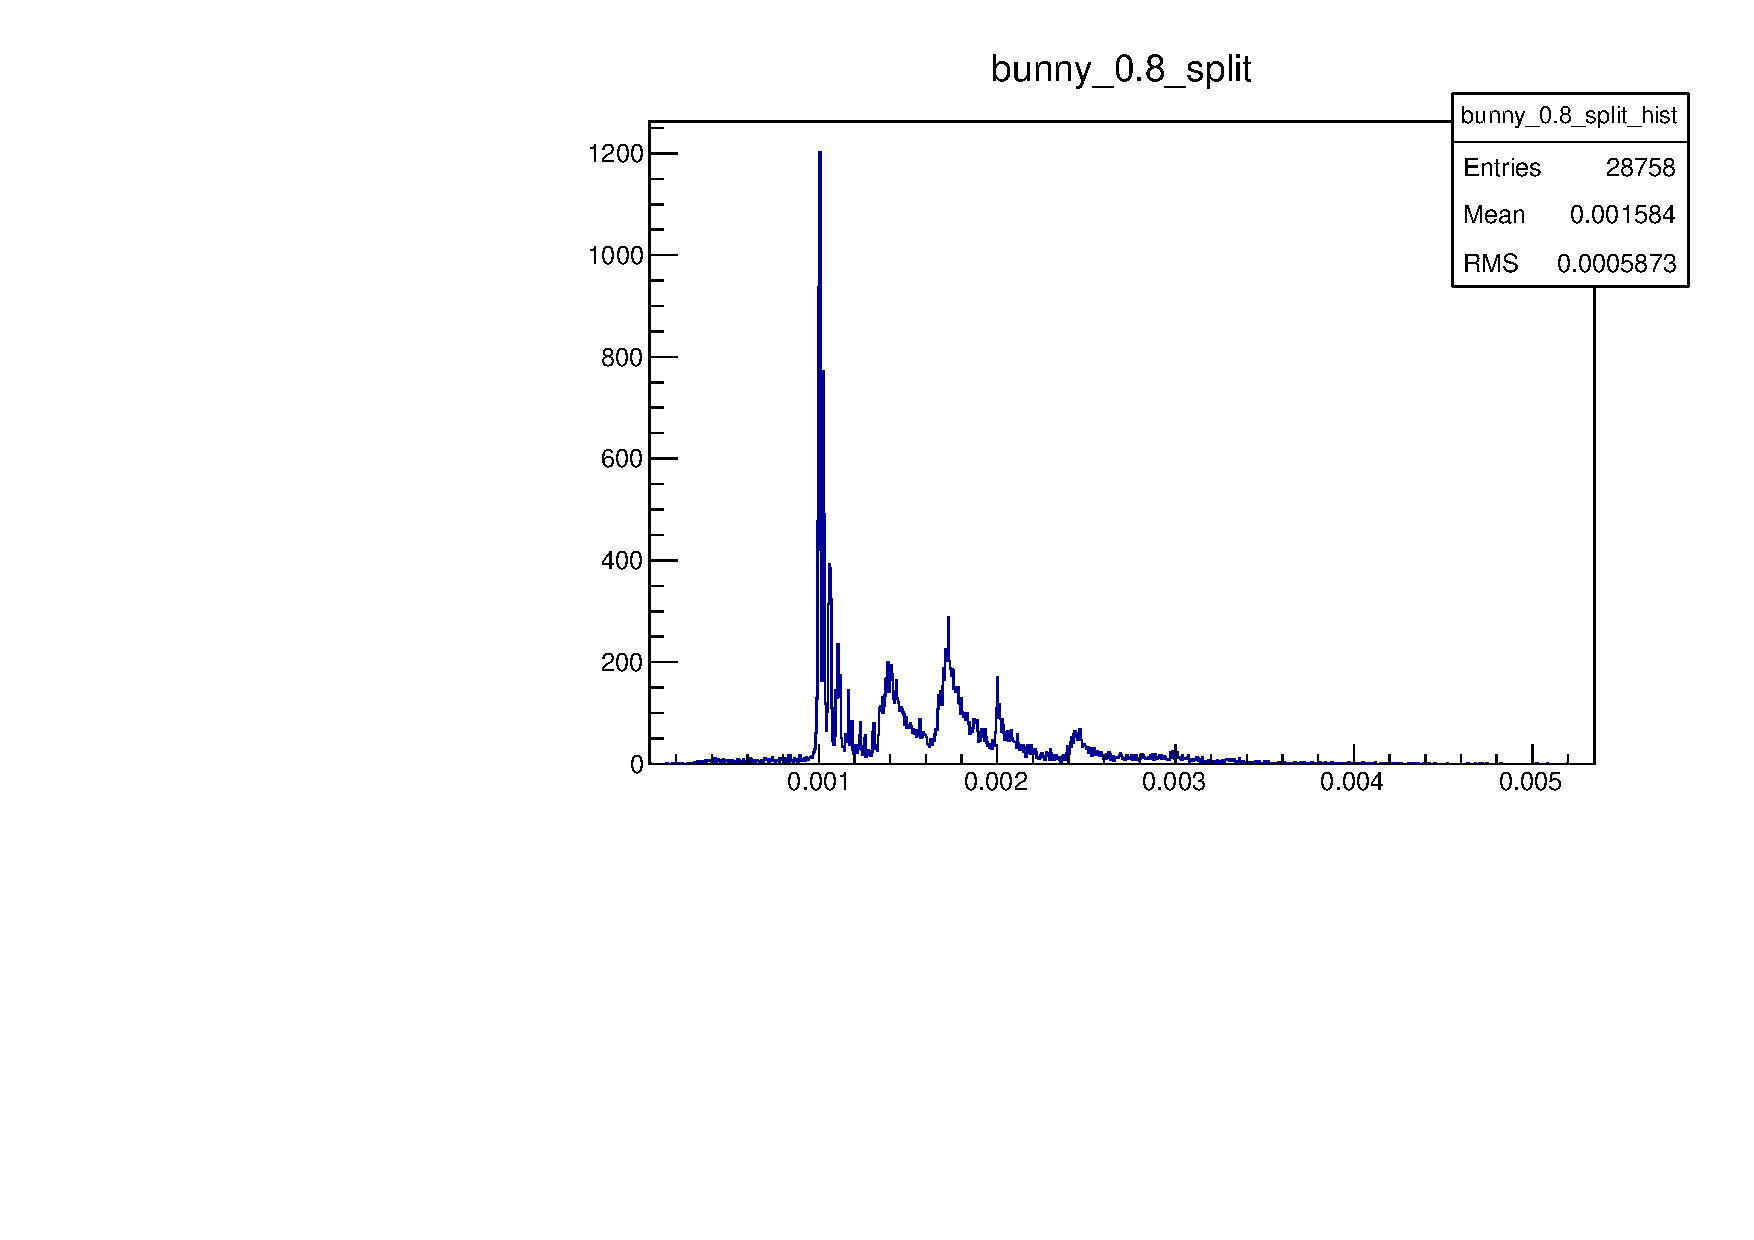
\includegraphics[width=\linewidth]{fig/bunny_08_split.pdf}
\end{subfigure}
\caption{Histograms of $\|q_i - p_i\|$ for 50\% and 80\% split}
\label{fig:bunny_fexp_before}
\end{figure}

In both cases, $\| q - p \| \approx 0.001$ is a mode in the distribution. Smaller values are infrequent. Additional spikes occur for some values above $0.001$. 

The reason is that for the original Bunny point clouds, the points are evenly distributed on the surface on an approximatively square grid, with a mean distance of about $0.001$ between adjacent points, as seen in the close-up view in figure \ref{fig:bunny_grid_closeup}. Figure \ref{fig:bunny_closest} shows a histogram made by taking from each point $p$ on the Bunny point cloud $B$, the closest point $p' \in B$ with $p' \neq p$. In the closest point histograms from $Q$ to $P$, any point that is in $Q$ is missing in $P$ and hence the closest point is often the one at a distance of $0.001$. Some instances appear where this point is not in $P$ either, so the closest point is further. This explains the spike at $0.002$. The other spikes occur when the closest point is in a diagonal direction on the grid. This ``grid'' is approximate and the surface is embedded in a non planar way in 3D space, so most samples do not fall exactly in one of these spikes.

For the true correspondences, the histogram would be a single spike at $\|p_i - q'_i\| = 0$. 

\begin{figure}[h]
\centering
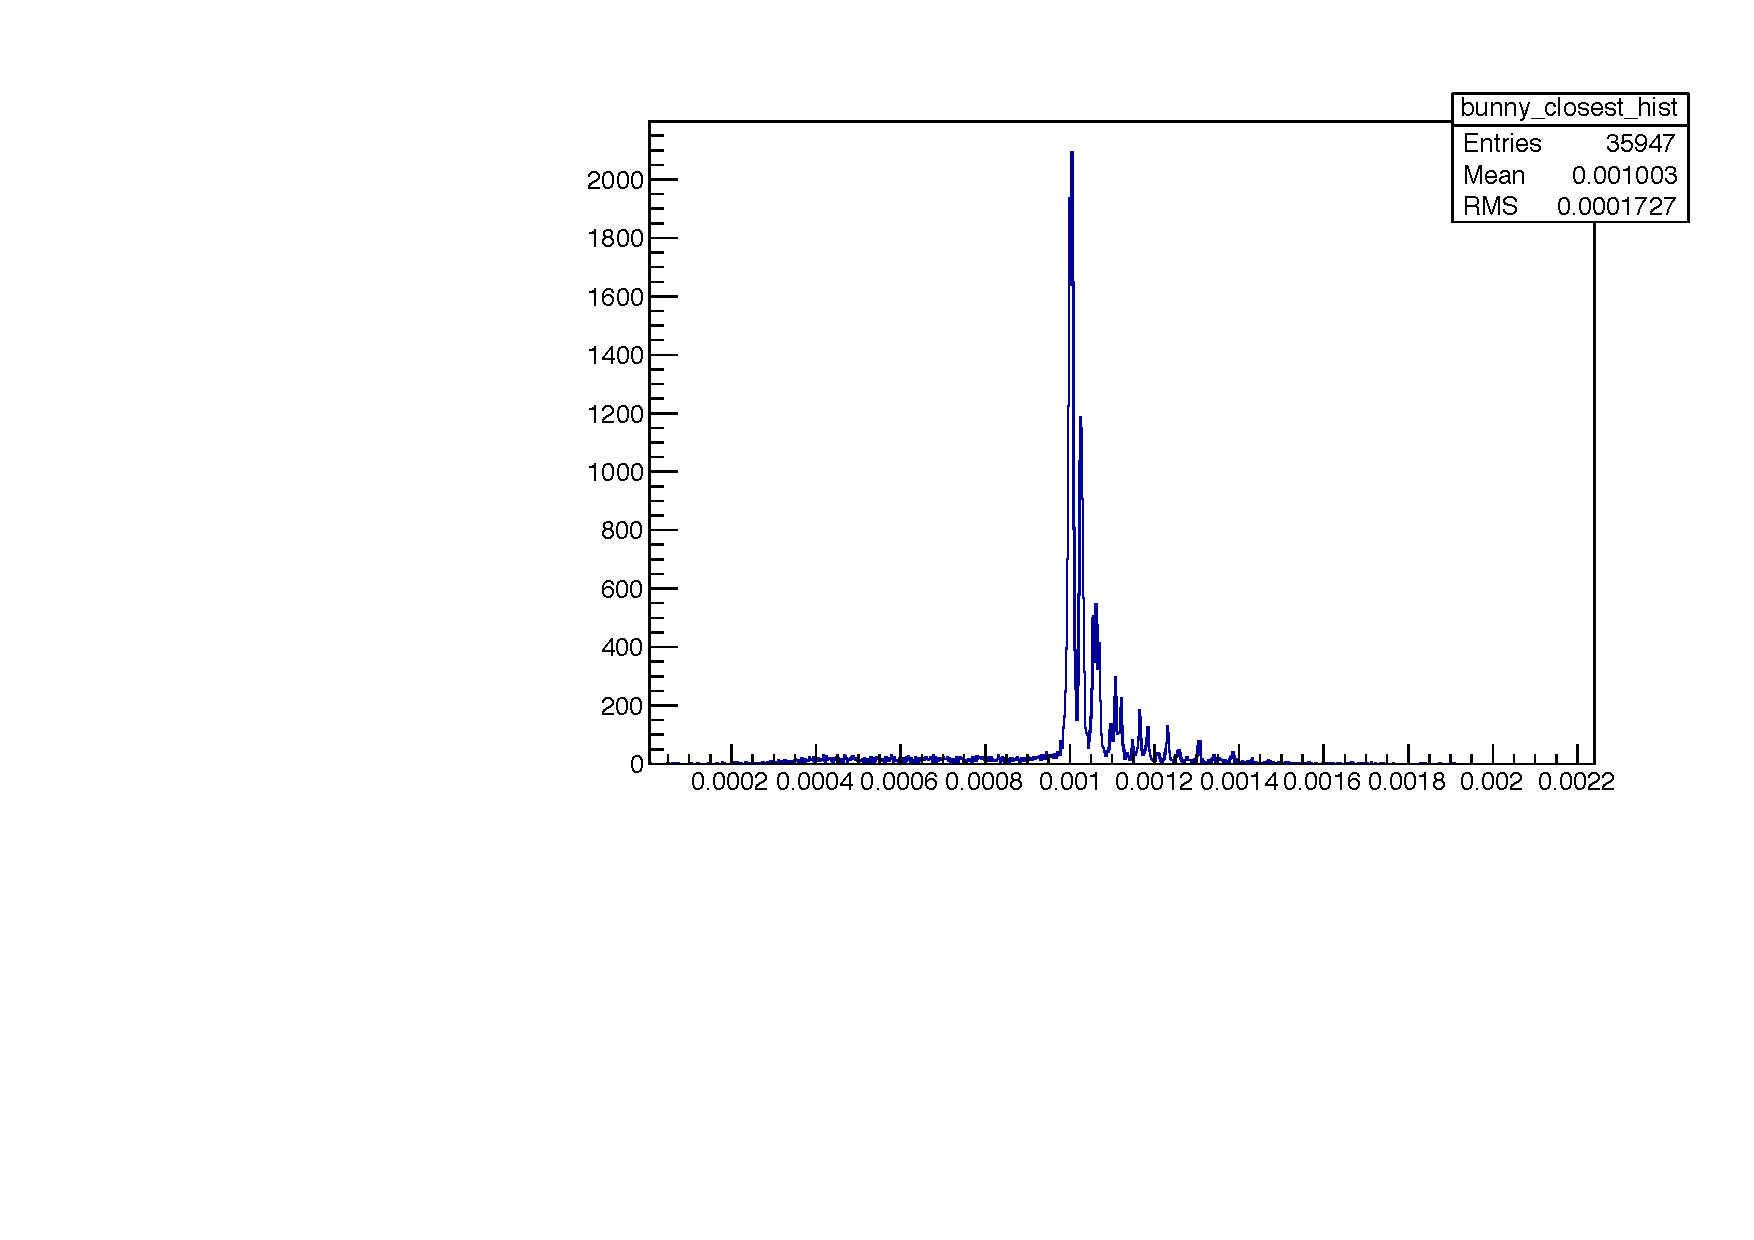
\includegraphics[width=.5\linewidth]{fig/bunny_closest.pdf}
\caption{Nearest neighbor distance histogram on Bunny point cloud}
\label{fig:bunny_closest}
\end{figure}

\subsubsection{Sphere experiment}
The same experiment was run on artificially generated sphere point clouds, where the points are randomly dispersed on the sphere surface at a given density. Both the number of points on the fixed and on the loose point clouds are varied. Because of the random dispersion they never coincide. 

In appendix \ref{sec:ex_sphere_hilo} the results are shown. The X-axis on the plot shows the \emph{maximal} number of points, of the loose point clouds and of the fixed point cloud. Initially the point clouds are perfectly aligned, and they deviate from that alignment during \gsl{icp} registration.

It can be seen that the mean error, and its variance are slightly larger when fewer points are involved, because the point dispersion is less dense on the surfaces, and so the nearest neighbor distances get greater. However, because the points here are dispersed randomly, there is already a high variance in the nearest neighbor distances, as will be shown later.

\subsubsection{Conclusion}
It can be concluded that the accuracy of registration that one can hope to attain with the \gls{icp} point-to-point error metric is limited by the density with which points are dispersed on the object surfaces. For this point cloud the final \emph{true error} after \gls{icp} registration tends to be off in average by the side length of the square grid which the points form.


\subsection{Different view points}
Another experiment was run to test \gls{icp}'s sensitivity to occlusion caused by different camera angles. A relief model as described in \ref{sec:relief} is used. The fixed and loose point clouds are both generated by generating a projected range image of it, with a camera placed at a higher altitude, looking down on the relief, and placed at an angle $\theta$ relative to the Y axis. For both the loose and the fixed point cloud these angles $\theta_{\text{fixed}}$ and $\theta_{\text{loose}}$ are independently varied from $0$ to $2 \pi$.

When $\theta_{\text{fixed}} = \theta_{\text{loose}}$ both point clouds feature the relief looked at from the same view point, thus there are no occluded parts from one point clouds relative to the other. As the difference gets greater the overlapping area gets smaller.

An example is shown on figures \ref{fig:relief_dproj}. On the first figure both point clouds are projected from the same view point. They are cropped to have different bounds, like point clouds from real scans would have. On the second figure the view point of the red point cloud is different.

Initially the fixed and loose point clouds are perfectly aligned, and then \gls{icp} is run. The final true error is recorded. The result is shown in appendix \ref{sec:ex_relief_dproj}. It can be seen that as the overlap gets smaller, \gls{icp} tends to converge towards an alignment that lays further off the true tranformation, even when the point clouds were perfectly aligned to start with.

Thus the global minimum of the error metric minimized by point-to-point \gls{icp} diverges from the true transformation.

\begin{figure}[h]
\centering
\begin{subfigure}{.5\textwidth}
	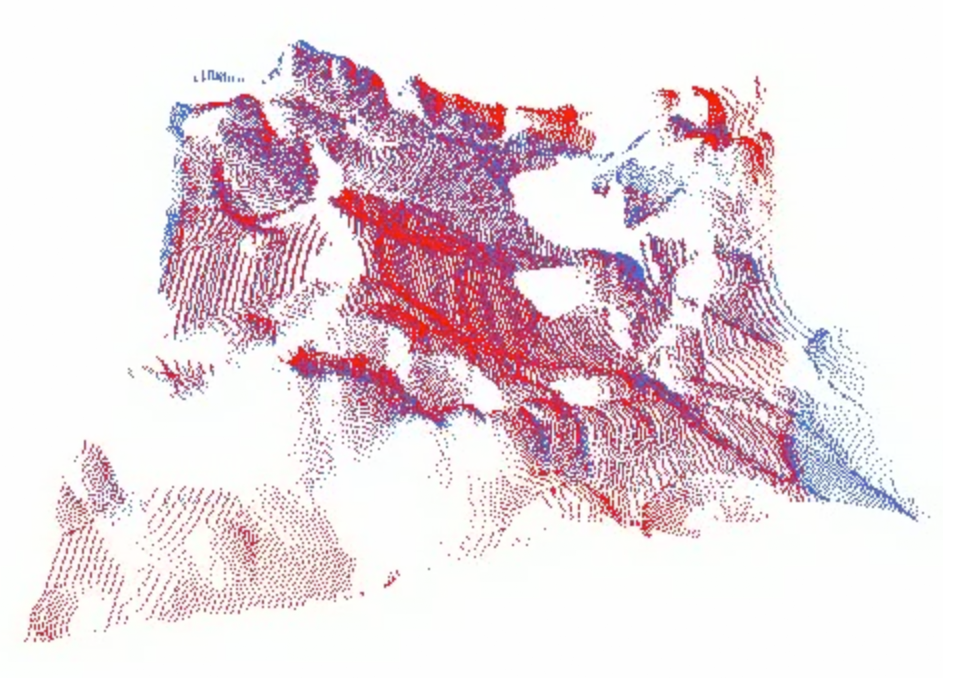
\includegraphics[width=\linewidth]{fig/relief_dproj_1.png}
	\caption{Same view point}
\end{subfigure}%
\begin{subfigure}{.5\textwidth}
	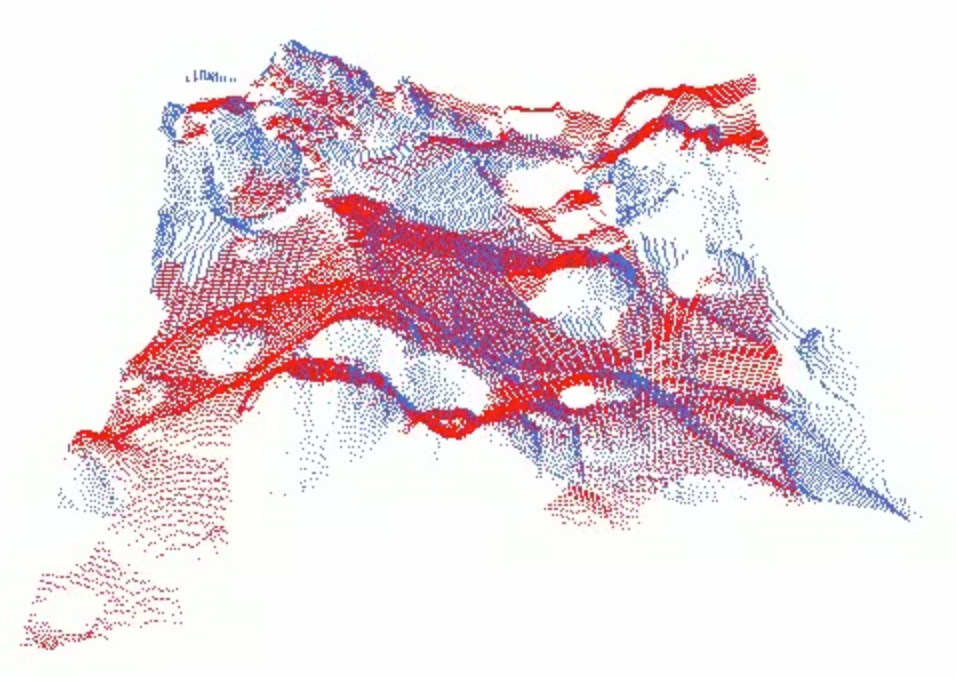
\includegraphics[width=\linewidth]{fig/relief_dproj_2.png}
	\caption{Different view points}
\end{subfigure}
\caption{Aligned relief point clouds, projected from different angles.}
\label{fig:relief_dproj}
\end{figure}


\subsection{Instability of error metric}
The experiment show that the point-to-point error metric used by \gls{icp} is unstable, in the sense that its accuracy deteriorates when one point cloud has lower resolution, and when they have low overlap due to different camera view poses.

Figure \ref{fig:relief_err} is a visualization of the \emph{mean absolute error} with closest-point correspondences, taken on a relief model. As explained before the curves show the value of $e(\matr{\hat{M}})$ for randomly chosen one-dimensional cross-sections of the rigid transformation space, such that $\matr{\hat{M}}$ is the true transformation $\matr{M}$ at $x = 0$. Therefore all the curves on the plots intersect at $x = 0$. An accurate error metric would have its global minimum at $x = 0$ and no local minima.

On these cross sections $\matr{\hat{M}}$ deviates from $\matr{M}$ by a maximum of $0.003$ translation length and $0.3\si{\degree}$ rotation angle. The relief model has a width of $5$ by comparison.

\begin{figure}[H]
\centering
\begin{subfigure}{.33\textwidth}
	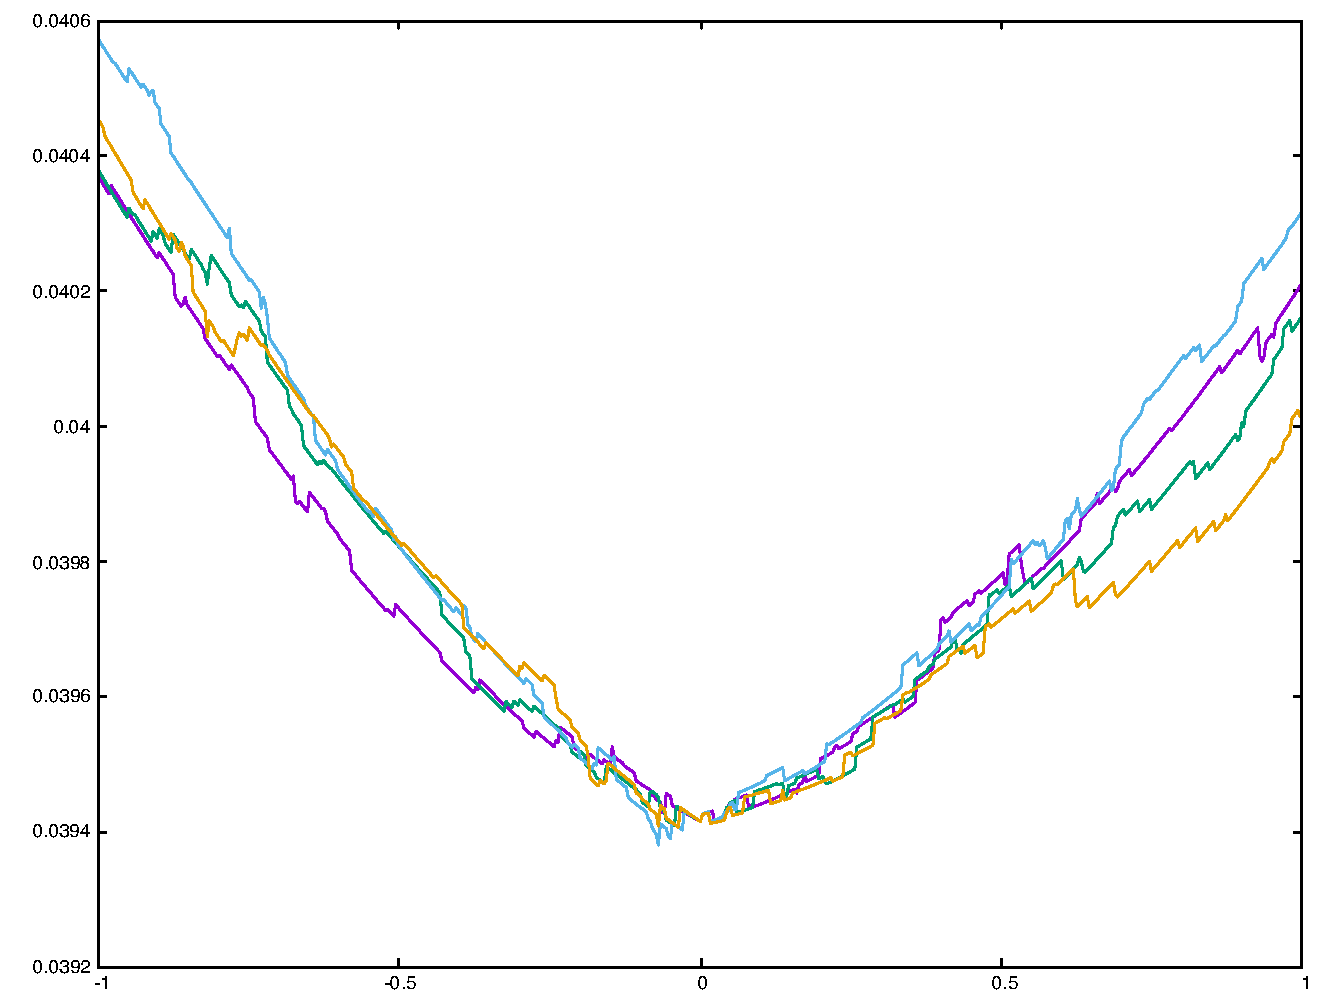
\includegraphics[width=\linewidth]{fig/relief_same_err.pdf}
	\caption{Same}
\end{subfigure}%
\begin{subfigure}{.33\textwidth}
	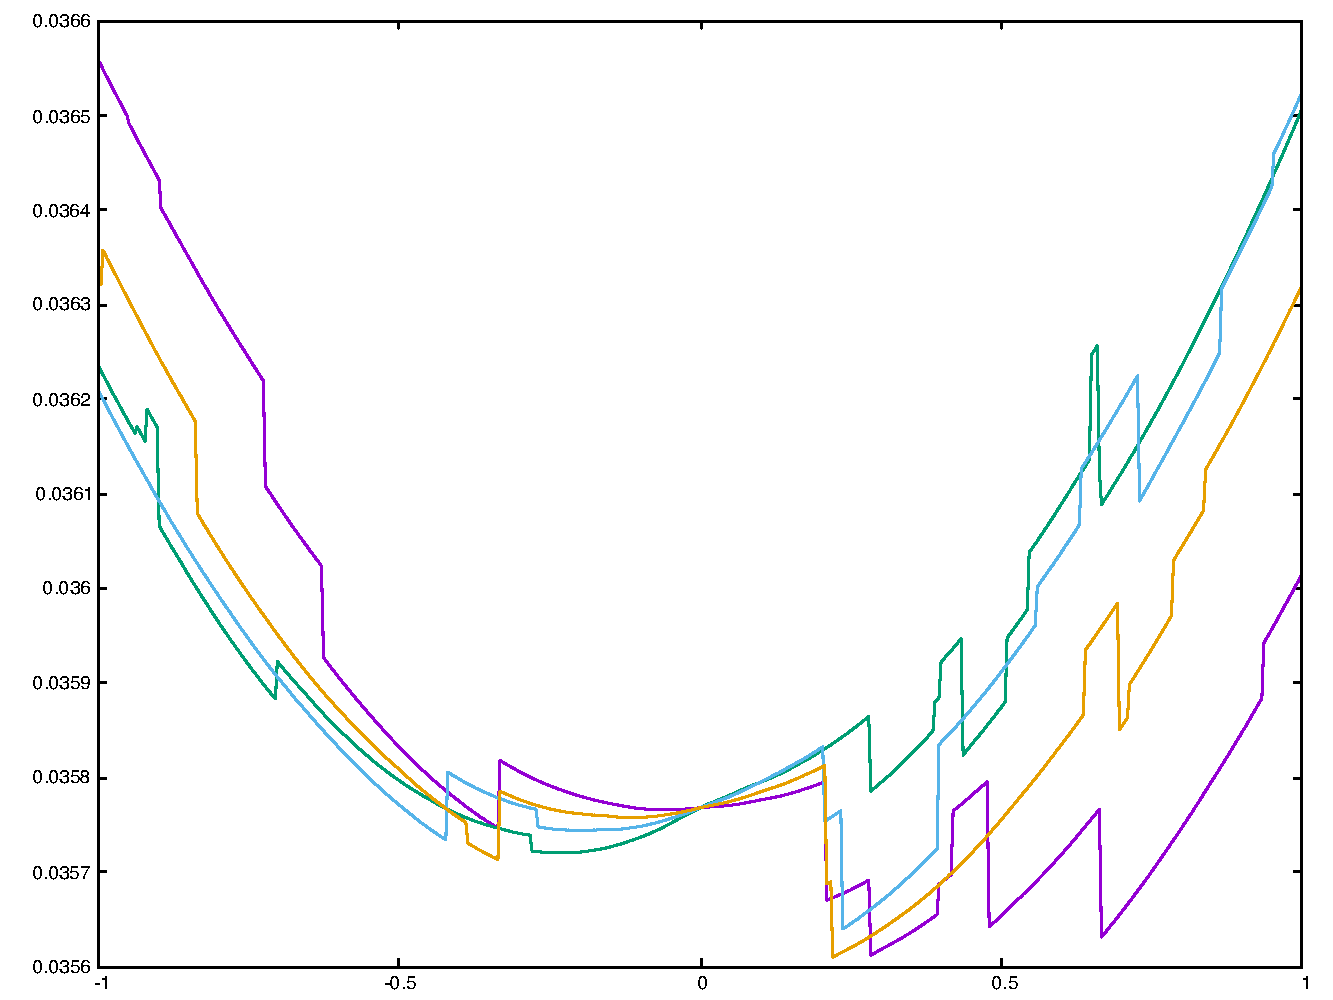
\includegraphics[width=\linewidth]{fig/relief_hilo_err.pdf}
	\caption{Different resolution}
\end{subfigure}
\begin{subfigure}{.33\textwidth}
	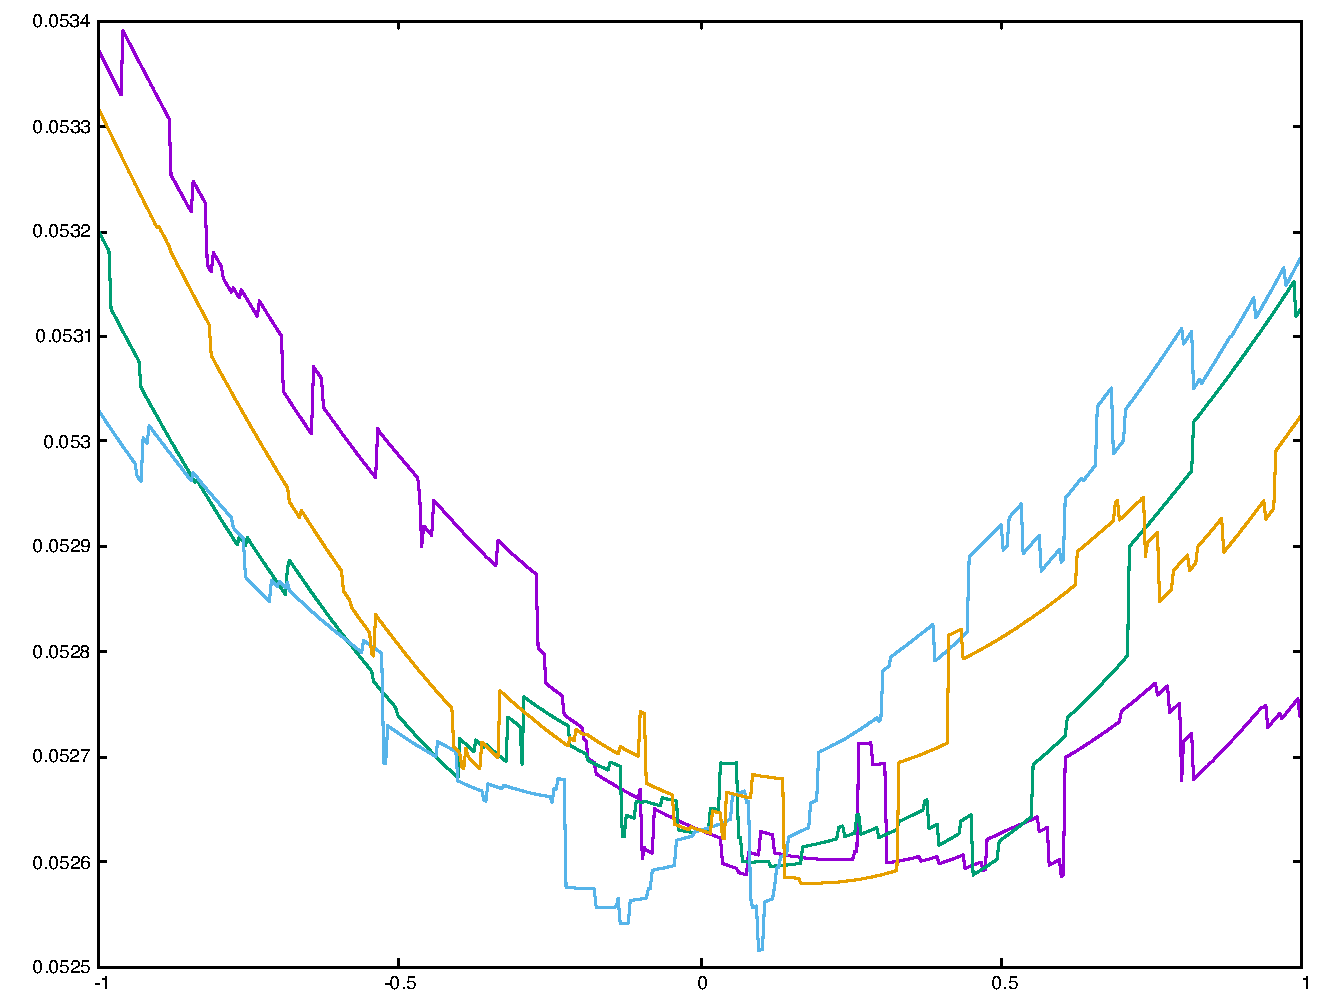
\includegraphics[width=\linewidth]{fig/relief_dproj_err.pdf}
	\caption{Different view-point}
\end{subfigure}
\caption{Mean absolute error metric visualization with closest-point criterion}
\label{fig:relief_err}
\end{figure}

In the first plot the fixed and loose point cloud have approximately the same resolution and total overlap, whereas in the other two cases their resolution or view-point has been altered like in the experiments. It can be seen that in those two cases, $\matr{M}$ is no longer the global minimum, and so \gls{icp} converges to another transformation as it did in the experiment runs.


\FloatBarrier

\newpage


\section{Developing an error metric}
Any error metric that does not use the true transformation is an \emph{estimation}, and its global minimum generally does not exactly coincide with the one from the \emph{true error}. But when the true transformation $\matr{M}$ is known, it can be directly compared with the \emph{true error}. An approach to develop a good estimative error metric is the following:
\begin{enumerate} 
\item First the scope is limited to point clouds having some \emph{characteristics} that the error metric will make use of.
\item An artificial 3D model which also has these characteristics is defined, along with an algorithm to generate artificial point clouds from it. On these point clouds, the true transformation is known, and parameters such as scanner noise and point errors can be simulated and controlled.
\item An estimative error metric is developed measures the alignment of two different point clouds generated from the model, without taking into account the true transformation $\matr{M}$, and based on the \emph{characteristics}. To evaluate its accuracy it is compared with the \emph{true error} metric.
\item When the estimative error metric works well enough, it is now applied to a real scan. It the artificial point clouds model the real scan well enough, it can be expected to still yield good results. Its accuracy is compared to the \emph{mean absolute error}, and evaluated manually by visual inspection.
\end{enumerate}

In this chapter, an attempt will be made to define a fine registration error metric, based on the histogram formed by the distances of point pairs chosen using the closest point criterion. For this the characteristic dispersion of points on the surfaces will be taken into account.

\subsection{High- to low-resolution registration}
The set goal was to improve registration when one point cloud has a lower resolution than the other. Naturally the first step is to develop an error metric which indicates when the point clouds are accurately registered. Then the second step is to develop an algorithm to find a transformation that minimizes this error metric.

This can be considered to be an ill-posed problem when the true transformation $\matr{M}$ is not known: Informally, an error metric attempts to extract information about $\matr{M}$, only from the two input point clouds $P$ and $Q$. When the number of points in $P$ is reduced, there is less information available. Now the goal is to find an algorithm such that $\text{register}(P, Q) = \matr{M}$, based only on the hypothesis that $\matr{M}$ exists. $P$ and $Q$ are data whereas the hypothetical $\matr{M}$ is a physical quantity. In other words it is not well defined what output the algorithm should produce. Point clouds taken from real 3D scans are very unstable data sets to work with because, as indicated in chapter \ref{ch:theory}, both the modeling of the object as a continuous surface and its representation using a set of points are approximations and imply that a degree of uncertainty is associated with every point.

\Gls{icp} with the closest-point criterion essentially relies on the expectation that for all the $q \in Q$, the divergences of a correspondence point $p$ to the true corresponding point $q'$ on the other surface $P$, will cancel each other out because to the large number of points $q$. If the number of points gets lower, this will no longer be the case.

Intuitively, in order to obtain a better error metric, more information about the surfaces needs to be extracted. Standard \gls{icp}'s view of the point cloud $P$ is limited to one corresponding point for each $q \in Q$. As shown in the previous chapter, many variants have been developed that take into account more information, such as the normal vectors, covariance matrices of the error, point attributes, etc.

\subsubsection{Approach}
Since the scope here is limited to range images, that have near-planar surfaces, the point dispersion pattern that the scanner's rays will produce on the surfaces can be considered to encode information about those surfaces. The following two point clouds are scans from the same object (dessus-de-porte).
\begin{figure}[H]
{
\centering
\setlength{\fboxsep}{0pt}%
\setlength{\fboxrule}{0.5pt}%
\hspace*{\fill}%
\begin{subfigure}{.48\textwidth}
	\fbox{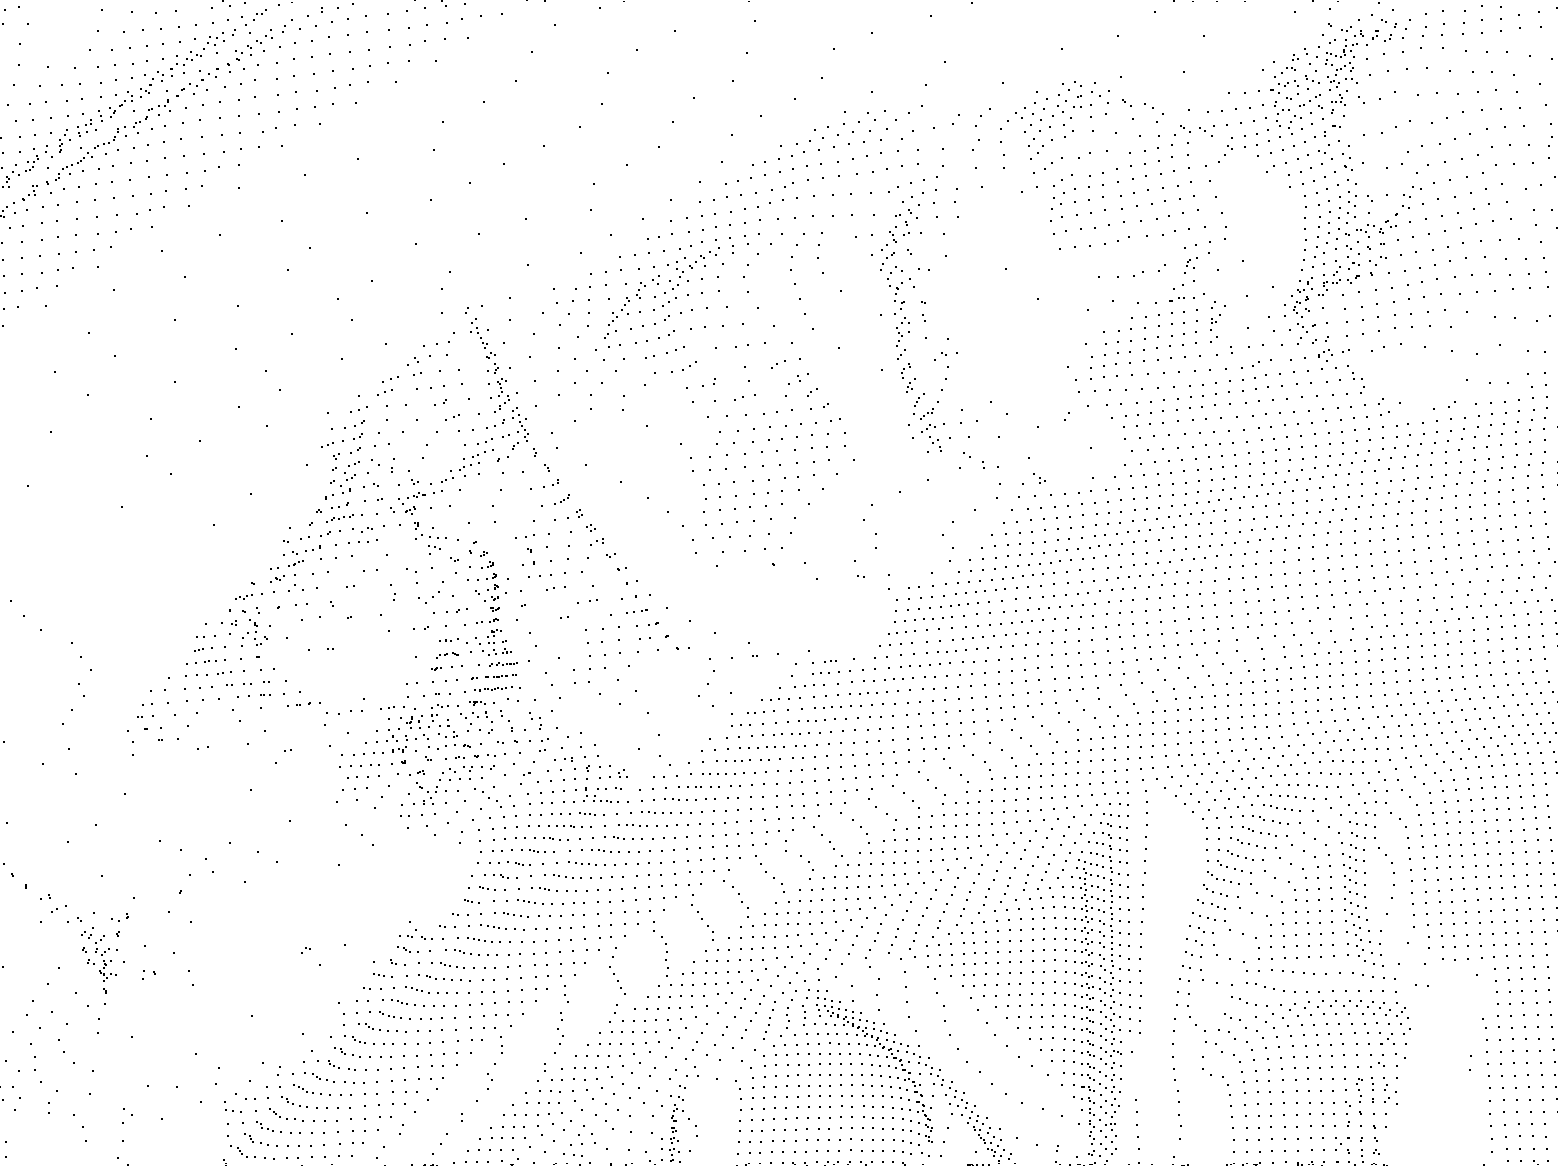
\includegraphics[width=\linewidth]{fig/idea_grid.png}}
	\caption{Points arranged on regular lattice}
\end{subfigure}%
\hfill%
\begin{subfigure}{.48\textwidth}
	\fbox{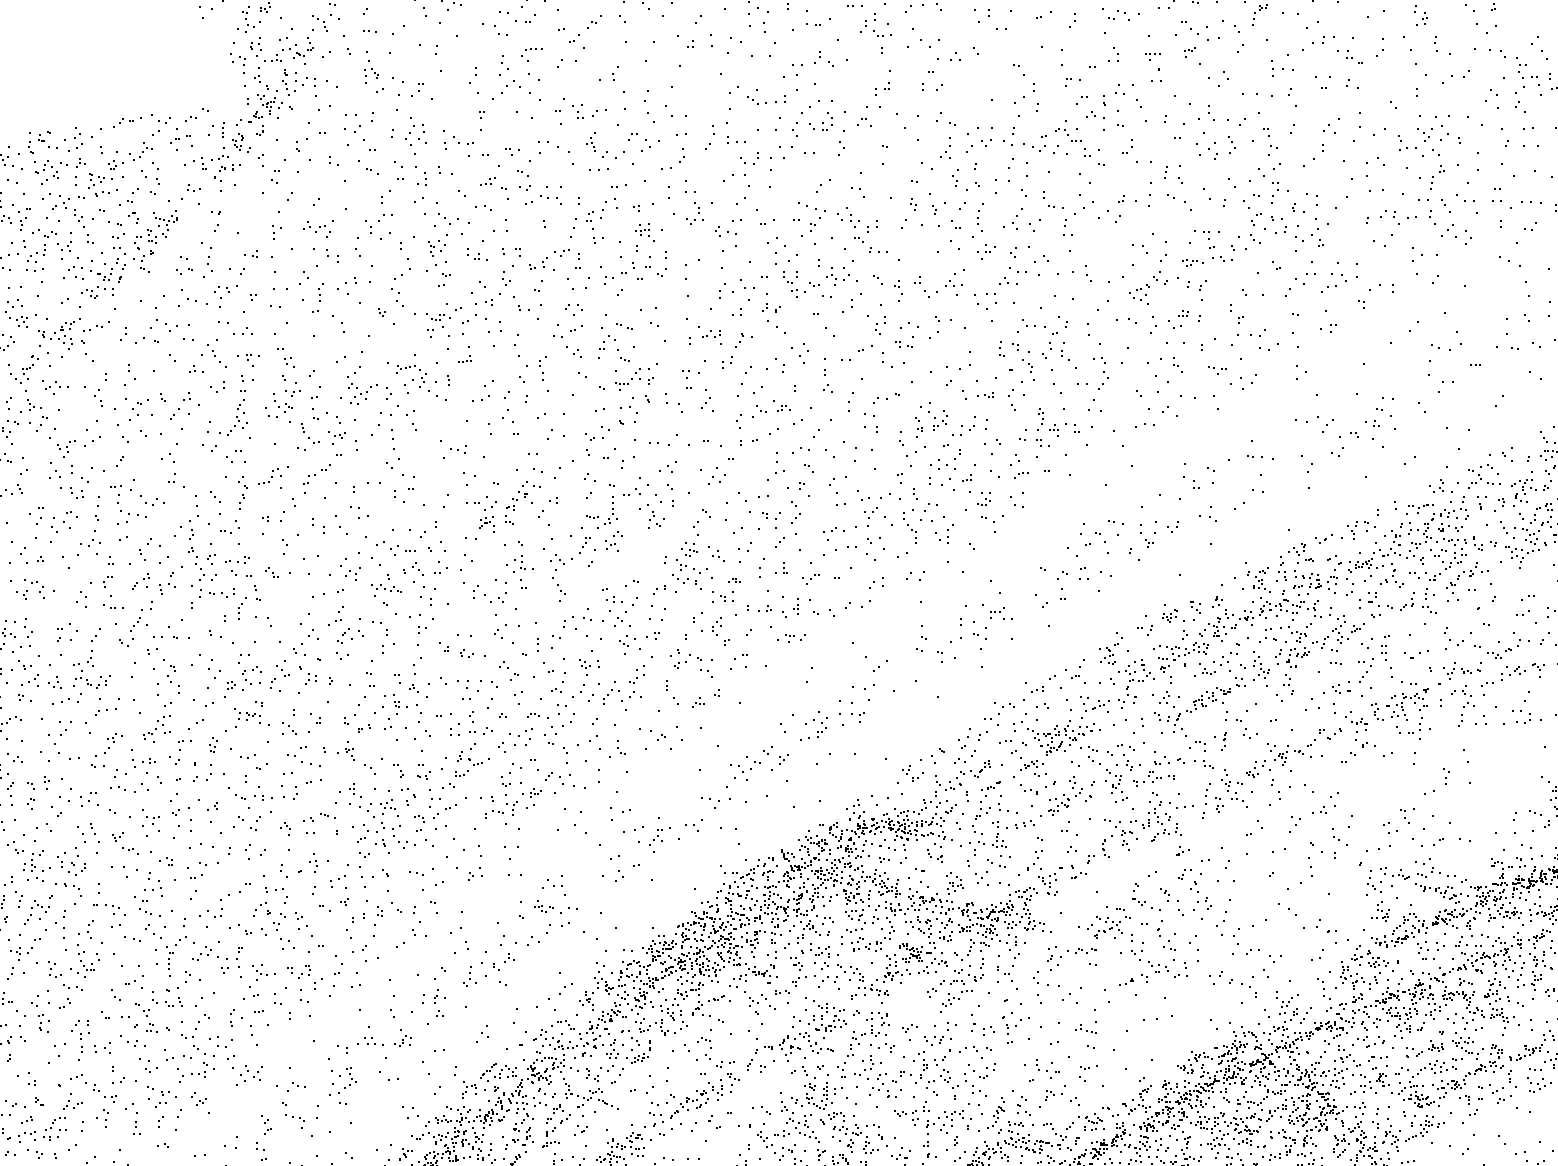
\includegraphics[width=\linewidth]{fig/idea_random.png}}
	\caption{Points dispersed randomly}
\end{subfigure}
}
\end{figure}

The first one shows the points' arrangement as produced by the scanner, whereas in the second one they are randomly dispersed, at about the same density.\footnote{It was generated from the higher resolution scan, followed by random downsampling} To a human looking at these two screenshots, is it immediately apparent that the first one contains more information about the object's geometry. To the point-to-point error metric, on the other hand, these two point clouds would ``look'' the same since it does not consider the positions of points in $P$ relative to one another.

The points become arranged so that they form a parallelogram lattice\footnote{will also be called a ``parallelogram grid'' in this paper} on planar surfaces of the object. When two point clouds $P$ and $Q$ of the same object, where $Q$ one if of higher resolution, are perfectly aligned and superimposed, points $q \in Q$ will fall between adjacent lattice points, and inside the parallelograms that they form.

The algorithm will record all of the distances from $q$ to the closest point $p \in P$ in a histogram. Only points $p$ that lie on locally planar surfaces are considered. At the same time, using the normal vectors of the points $p$ relative to the camera view ray directions, it is possible to predict properties of parallelogram lattice on which $p$ lies. This includes the probability distribution of the distance from any position on the same plane to the closest point of the lattice. This probability density function will be compared to the recorded histogram.

If $P$ and $Q$ are well aligned they should form the same distribution. If not, the distances on the histogram will be diverge more because an additional displacement in the third dimension relative to the surface is added. An error metric is extracted from the comparison of the histogram.

Unlike the point-to-point error metric, this looks at the \emph{distribution} of the distances and not just at the \emph{average}. The expected distribution is based on the lattice formed by the points $p \in P$ relative to one another.



\newpage

\section{Analysis of point clouds}
In this section the point clouds are looked at in more detail on a local per-point scale, including the dispersion pattern of points on the surfaces. Some local measures will be defined that assign to each point in the point cloud a value in relation with its surrounding points. A way to predict the dispersion of points will be developed.

\subsection{Local density}
The \emph{local surface density} $\rho(p)$ of a point cloud $P$ around a point $p \in P$ indicates how densely points are dispersed on the surface around $p$, expressed in number of points per surface area. Because the shape of the underlying surface is unknown, a precise measure cannot be defined, and instead an approximation is used.

Taking the $k$ nearest neighbors around a point $p$ that is in a region where the surface is approximately planar results in a set of points located approximately on a disk around $p$. In this case, an estimate for the density is $\rho(p) = \frac{k}{\pi \, r_{\text{max}}^2}$, where $r_{\text{max}}$ is the maximal distance of one of the neighbors to $p$.

Even when the surface is not locally planar in that region, some level of accuracy is retained because Euclidian distances in three-dimensional space are measured, which are approximatively equal to distances measured along the surface on which the disk would be wrapped.

Using $r_{\text{max}}$ makes the measure more sensitive to outliers, and can overestimate the density: $r_{\text{max}}$ by definition is the smallest least radius such that $k$ points are inside the disk. An alternative is to use the median $r_{\text{med}}$ of the radii, and set $\rho(p) = \frac{k}{2 \, \pi \, r_{\text{med}}^2}$. For the median value, half of the $k$ points have a smaller radius and are thus inside the disk.

When the density is supposed to be constant for each point in the point cloud, it will also be denoted as $\rho$ or $\rho(P)$.

\subsubsection{Square grid density}
For artificially generated point clouds, per-point densities $\rho(p)$ are set to their theoretical values. For a planar surface where points are arranged on a square grid with side length $l$, this density is $\rho(p) = \frac{1}{l^2}$, because $1$ point can be counted per square. This will be extended to parallelogram grids in the next section.


\subsection{Local curvature} \label{sec:curvature}
In the rest of this chapter, properties of the dispersion of points on planar surfaces of the model will be used. It is therefore important to distinguish between approximatively planar regions of the surface, and more sharp edges.

Unlike the density, this is a measure of the surface and not of the point dispersion on it. This implies that the metric should be invariant of the point dispersion. In addition to this, it is dependent on a scale parameter: for example a point cloud representing a wall of a building would be planar on a scale of a few centimeters, but not on a millimeter scale where the texture of the wall is considered.

A measure of \emph{local curvature} $c(p, r)$ around a point $p \in P$ with a radius $r \in \mathbb{R}$ will be defined. A tangent plane is attached to the point $p$, with the same normal vector $\vec{n}$ as the point. This normal vector is assumed to have been calculated beforehand, for example by least-squares of \gls{ransac} plane fitting. Then it is measured how well the neighboring points fit on the plane.

Using the local density $\rho(p)$, the expected number of points located in a radius $r$ on the surface is $\rho(p) \, \pi \, r^2$. Using a kNN algorithm the $k = \lceil \rho(p) \, \pi \, r^2 \rceil$ nearest neighbors $N_k \subset P$ are searched. When $k$ is below a predefined threshold it is increased to a minimal value. This is for example the case on oblique surfaces where the density is lower and the nearest neighbor distances get larger.

If the surface is locally planar around and $p$ in the given radius, the points $N_k$ will be located in a disk around $p$, with a radius of approximatively $r$. Because the circumference of a circle is proportional to its radius, $N_k$ contains more points at higher radii, and the probability density of their distance to $p$ increases linearly. But these points at a higher distance that fit on the plane should not overcompensate for nearer points that don't. Weights are attributed to the points to cancel out that effect: The weight of the closest point $p_1$ is set to $1$, and those of the remaining points $p_i$ to $\frac{\| p_1 - p \|}{\| p_i - p \|}$. Then the weights are normalized to sum up to $1$.

To measure how well a point $p_i \in N_k$ fits the plane, two values are useful: Its distance $d_i$ to the plane, and the absolute angle $|\alpha_i|$ between its normal vector and that of the plane. Both can be calculated using the dot products:
\begin{equation}
d_i = \vec{n} \, (\vec{p_i} - \vec{p})
\hspace{7mm} \text{and} \hspace{7mm}
\cos \alpha_i = \vec{n} \, \vec{n_i}
\end{equation} 

The local curvature metric is calculated as weighted average of those values for the $k$ neighboring points:
\begin{equation}
c(p, r) = \frac{1}{k} \sum_{i=1}^{k} w_i \, \left( A \, |\alpha_i| + D \, d_i \right)
\end{equation}
where the coefficients $A$ and $D$ are set so as to attribute different weights to the two measures. To avoid evaluating $\arccos$ for each point, the angle can be approximated using $\alpha'_i = \frac{\pi}{2} (1 - \vec{n} \, \vec{n_i})$. These two figures show two surfaces (in two dimensions) where one metric it high and the other low.
\begin{figure}[H]
\centering
\begin{subfigure}{.4\textwidth}
	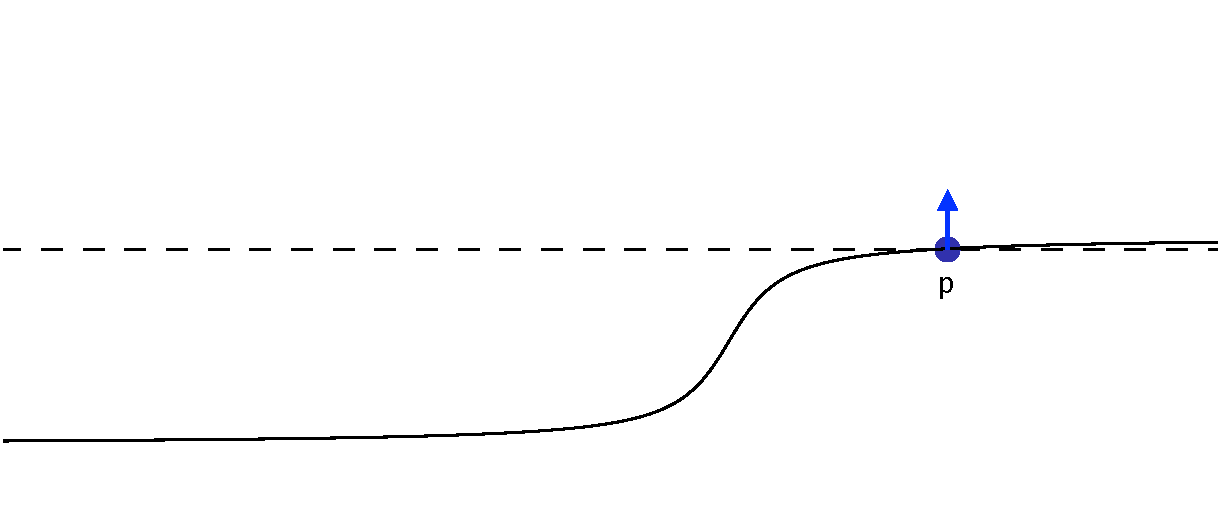
\includegraphics[width=\linewidth]{fig/curvature_distances.pdf}
	\caption{Large $\sum d_i$, small $\sum |\alpha_i|$}
\end{subfigure}%
\hspace{15mm}%
\begin{subfigure}{.4\textwidth}
	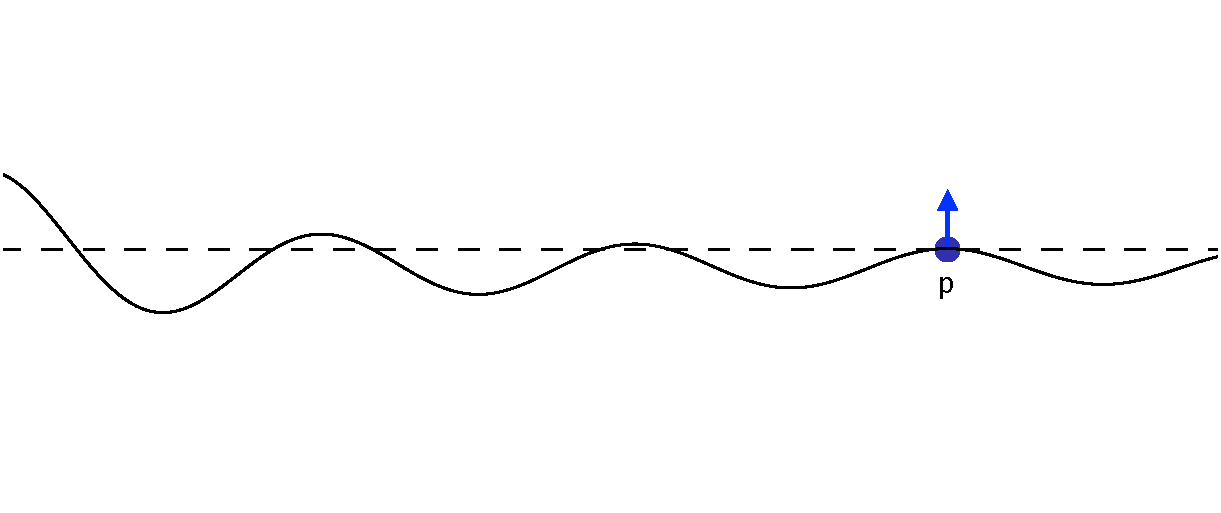
\includegraphics[width=\linewidth]{fig/curvature_angles.pdf}
	\caption{Large $\sum |\alpha_i|$, small $\sum d_i$}
\end{subfigure}	
\end{figure}
For the purposes that the curvature measure is used here, $A$ should be set higher, because surfaces such as the left-side can still be considered to be locally planar.

In figure \ref{fig:curvature_example} the ``dessus-de-porte'' scan is shown with points colorized according to this curvature measure. The color scale is shown on the figure. The blue and green parts indicate lower curvature, and thus more planar surface. It can be seen that the straight wall in the background is identified as being more planar, whilst rounded surfaces of the stone figures get a higher curvature value. Here $A = 10$ and $D = 3$, and $r = 0.01$ is used. The scale ranges from $c(p, r) = 0.000$ to $0.003$.


\begin{figure}[p]
\centering
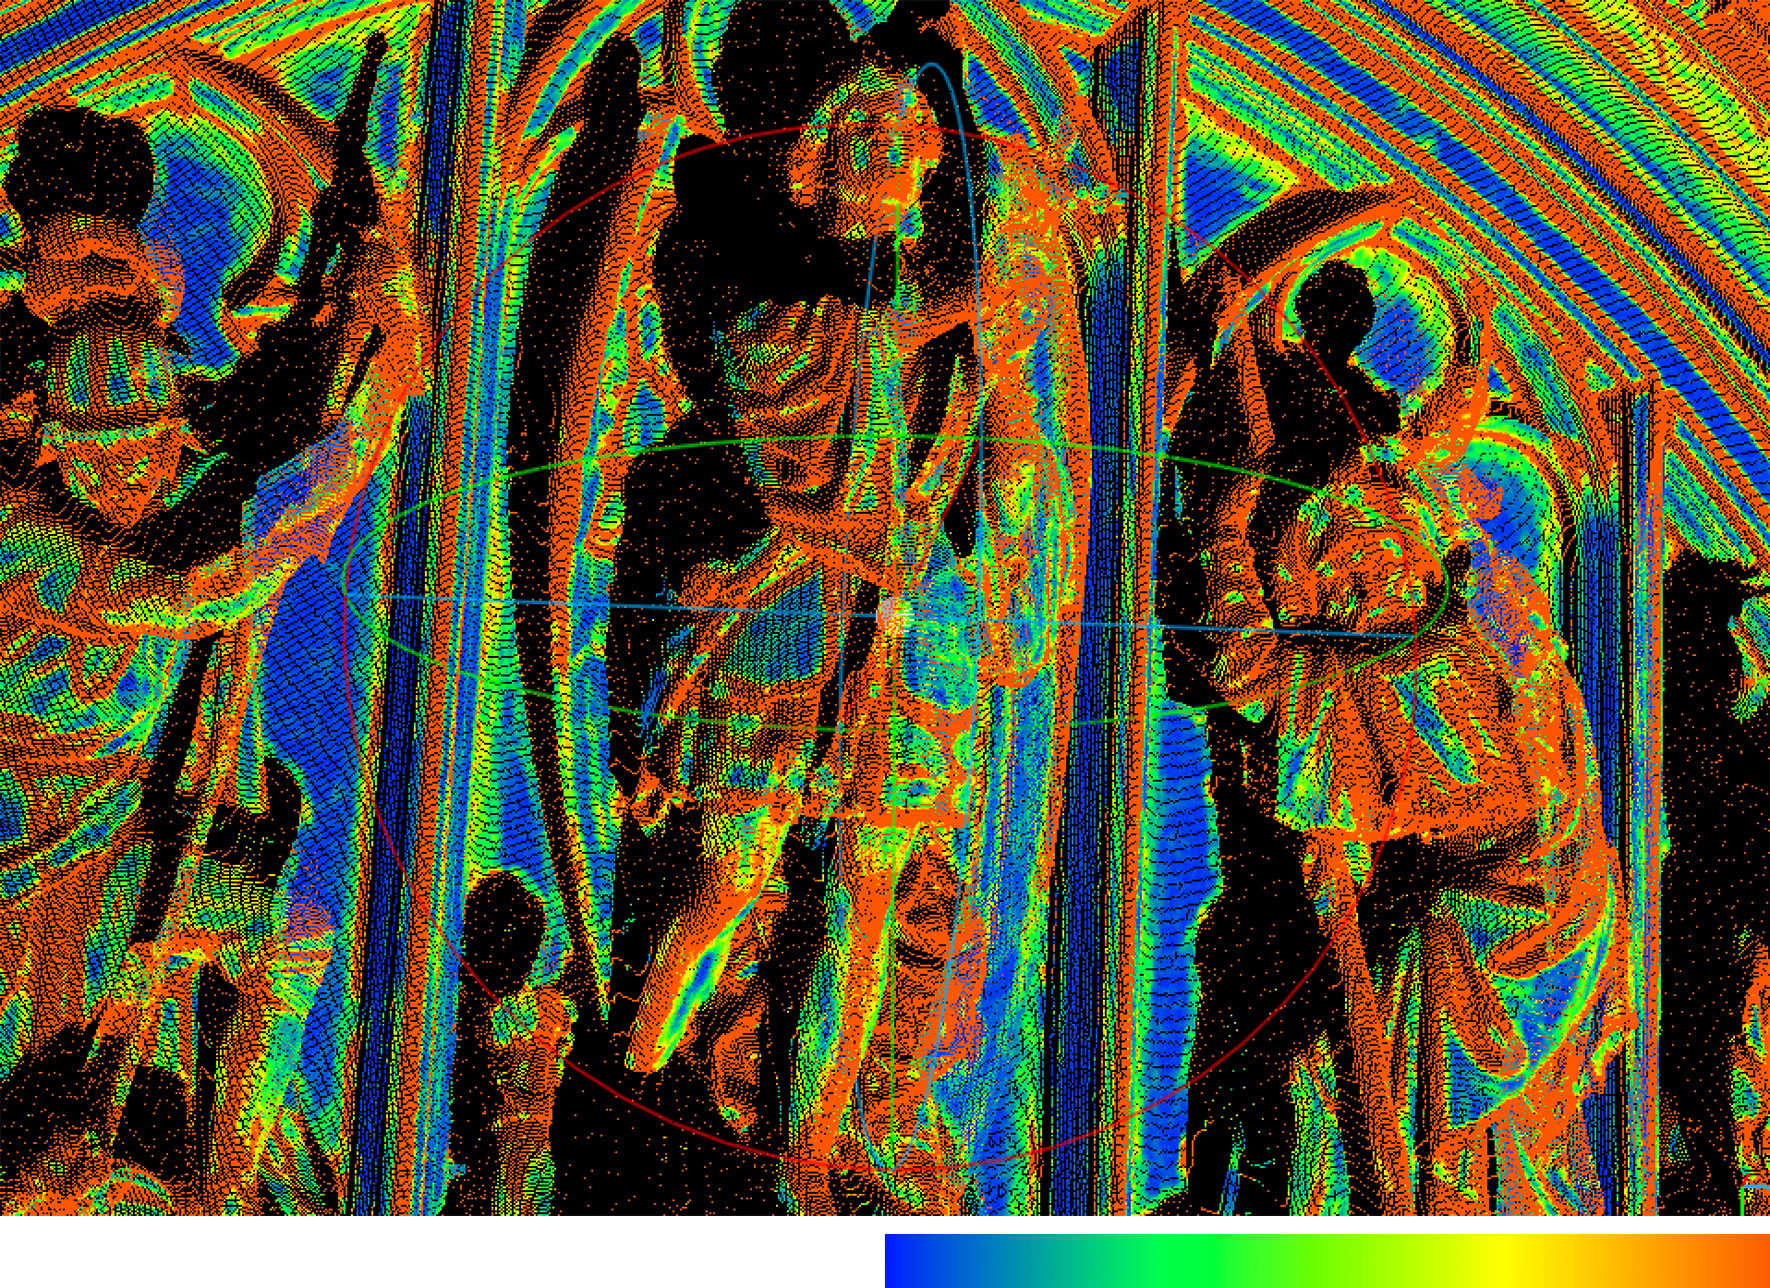
\includegraphics[width=.7\textwidth]{fig/curvature_example.png}
\caption{Example point cloud colorized according to curvature measure}
\label{fig:curvature_example}
\end{figure}



\subsection{Point dispersion}
Point dispersion refers to how points in a point clouds are arranged on a surface. When the surface is locally planar, regions of the surface can be approximated by a plane. The following three point dispersions on the plane will be analyzed:
\begin{figure}[H]
\centering
\hspace*{\fill}%
\begin{subfigure}{.3\textwidth}
{
	\setlength{\fboxsep}{0pt}%
	\setlength{\fboxrule}{0.5pt}%
	\fbox{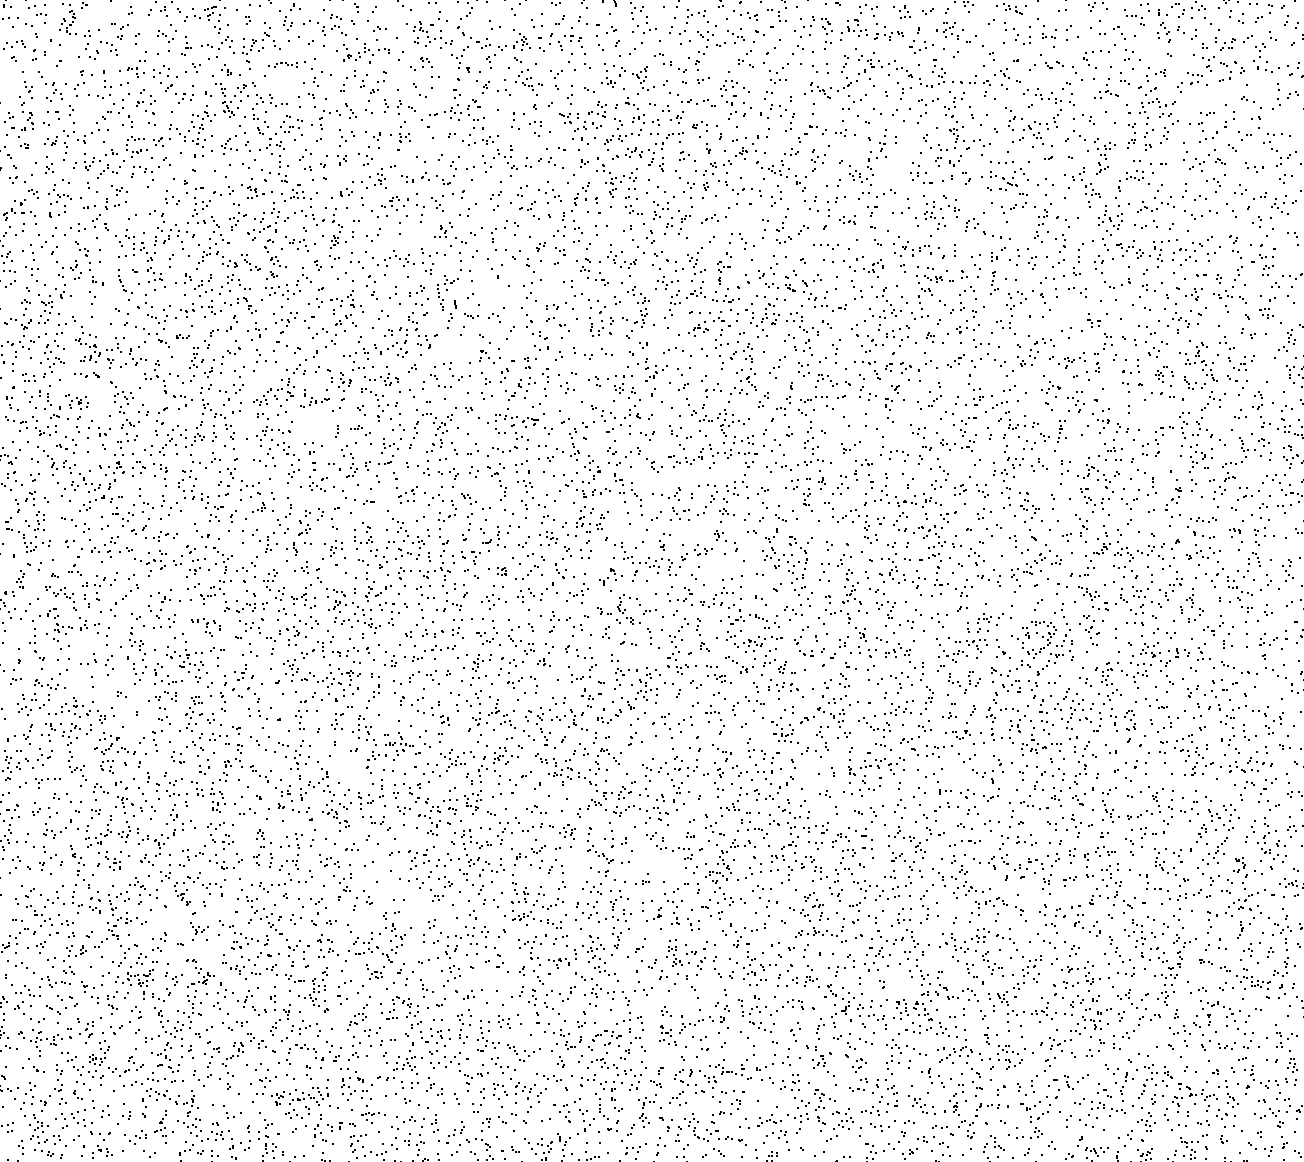
\includegraphics[width=\linewidth]{fig/dispersion_random.png}}%
	\caption{Random dispersion}
}
\end{subfigure}%
\hfill%
\begin{subfigure}{.3\textwidth}
{
	\setlength{\fboxsep}{0pt}%
	\setlength{\fboxrule}{0.5pt}%
	\fbox{
\includegraphics[width=\linewidth]{fig/dispersion_sqgrid.png}}%
	\caption{Square grid}
}
\end{subfigure}%
\hfill%
\begin{subfigure}{.3\textwidth}
{
	\setlength{\fboxsep}{0pt}%
	\setlength{\fboxrule}{0.5pt}%
	\fbox{
\includegraphics[width=\linewidth]{fig/dispersion_pargrid.png}}%
	\caption{Parallelogram grid}
}%
\end{subfigure}\\
\caption{Different point dispersions on planar surface}
\label{fig:point_dispersion}
\end{figure}

The \emph{random dispersion} is the most general case, where the $x$ and $y$ coordinates of each points are independent, random variables, with a uniform distribution. It can be seen visually that the local density in that case is not constant.

Point clouds recorded by a laser scanner will produce a dispersion that is more akin to the \emph{square grid dispersion}. If the scanner processes in sequential scan-lines, and uses a regular graduation of azimuth and elevation coordinates, a planar surface placed perpendicular to the scanner ray will \emph{locally} get points approximatively arranged in squares. The dispersion will be considered to be invariant to a two-dimensional rotation of the plane itself.

\subsection{Parallelogram grid}
When the surface is placed at an oblique angle to the scanner line, the points on the plane will instead be dispersed on a \emph{parallelogram grid}. Figures \ref{fig:closeup_ddp}, \ref{fig:closeup_wall} show two close-up views from the ``Hôtel de Ville'' scans, featuring the parallelogram grid point dispersion on approximatively planar surfaces. Figure \ref{fig:bunny_grid_closeup} is taken from the Stanford Bunny point cloud, which was also recorded using a laser scanner. A square grid or rectangular grid are special case of this.

\begin{figure}[p]
\centering
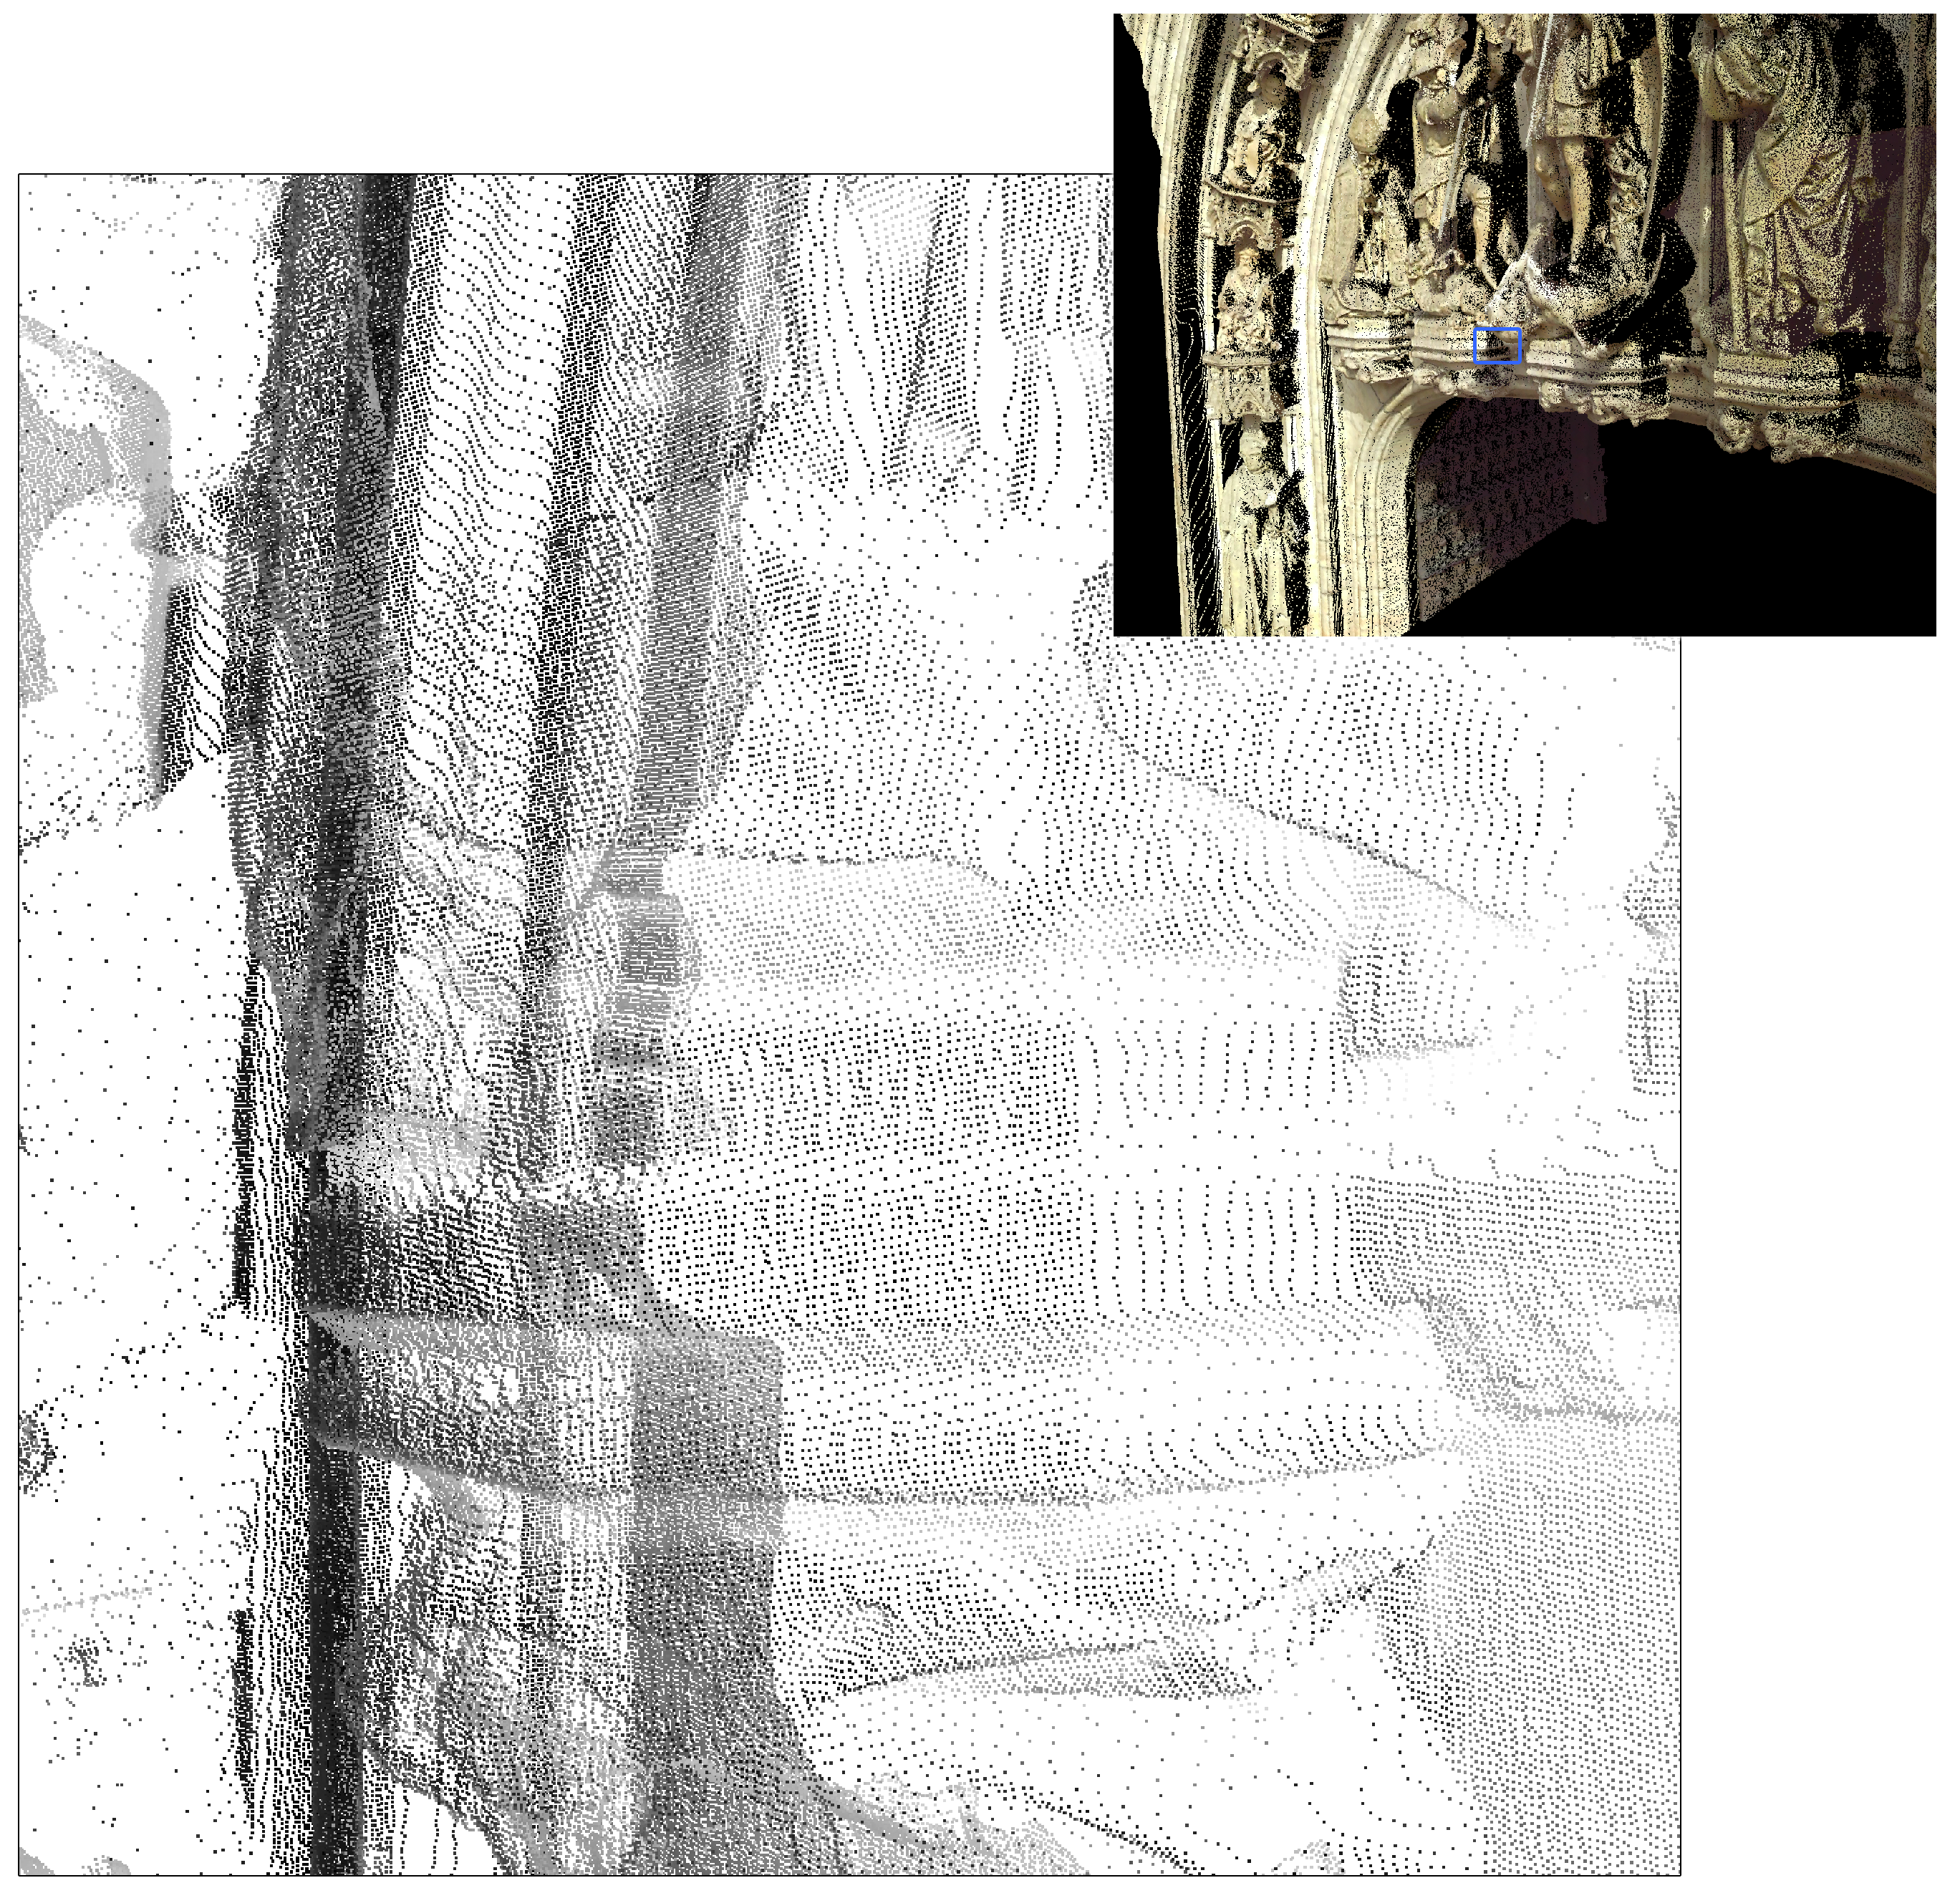
\includegraphics[width=.6\textwidth]{fig/closeup_ddp.png}
\caption{Closeup of the surface distribution of points on front wall of building}
\label{fig:closeup_ddp}
\end{figure}

\begin{figure}[p]
\centering
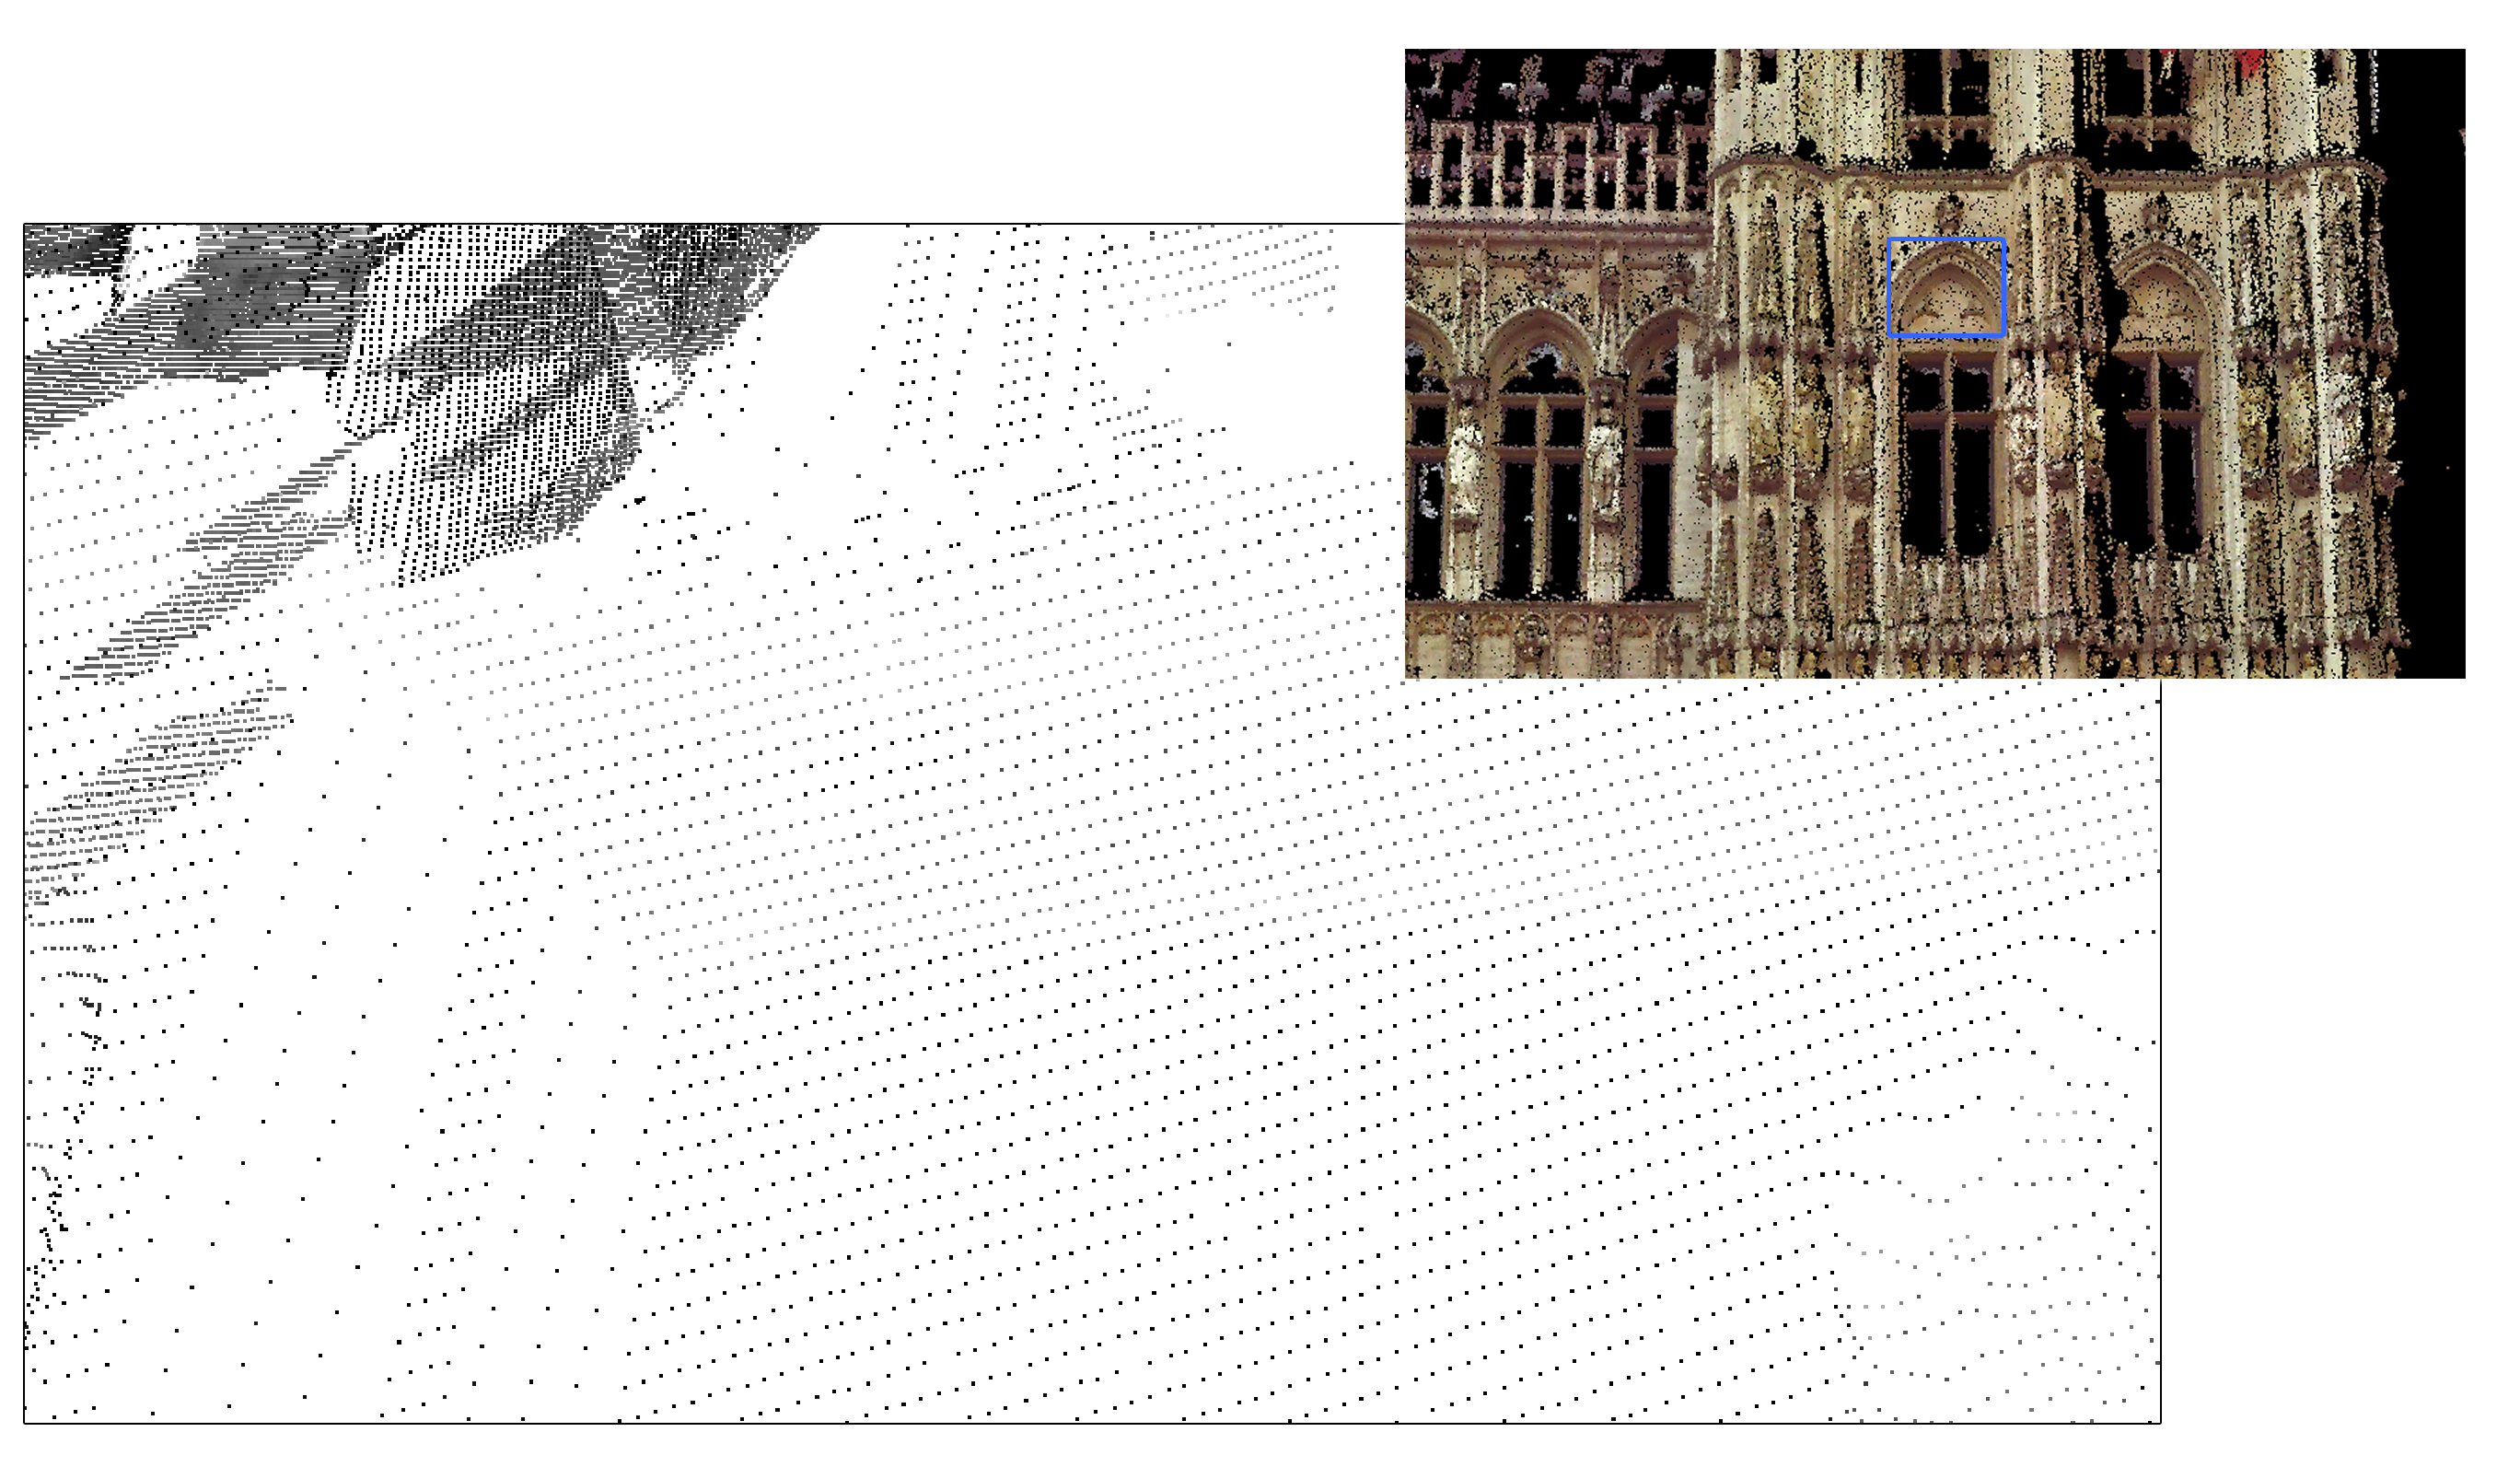
\includegraphics[width=.6\textwidth]{fig/closeup_wall.png}
\caption{Closeup of the surface distribution of points on detail of ``dessus-de-porte''}
\label{fig:closeup_wall}
\end{figure}

\begin{figure}[p]
\centering
{
	\setlength{\fboxsep}{0pt}%
	\setlength{\fboxrule}{0.5pt}%
	\fbox{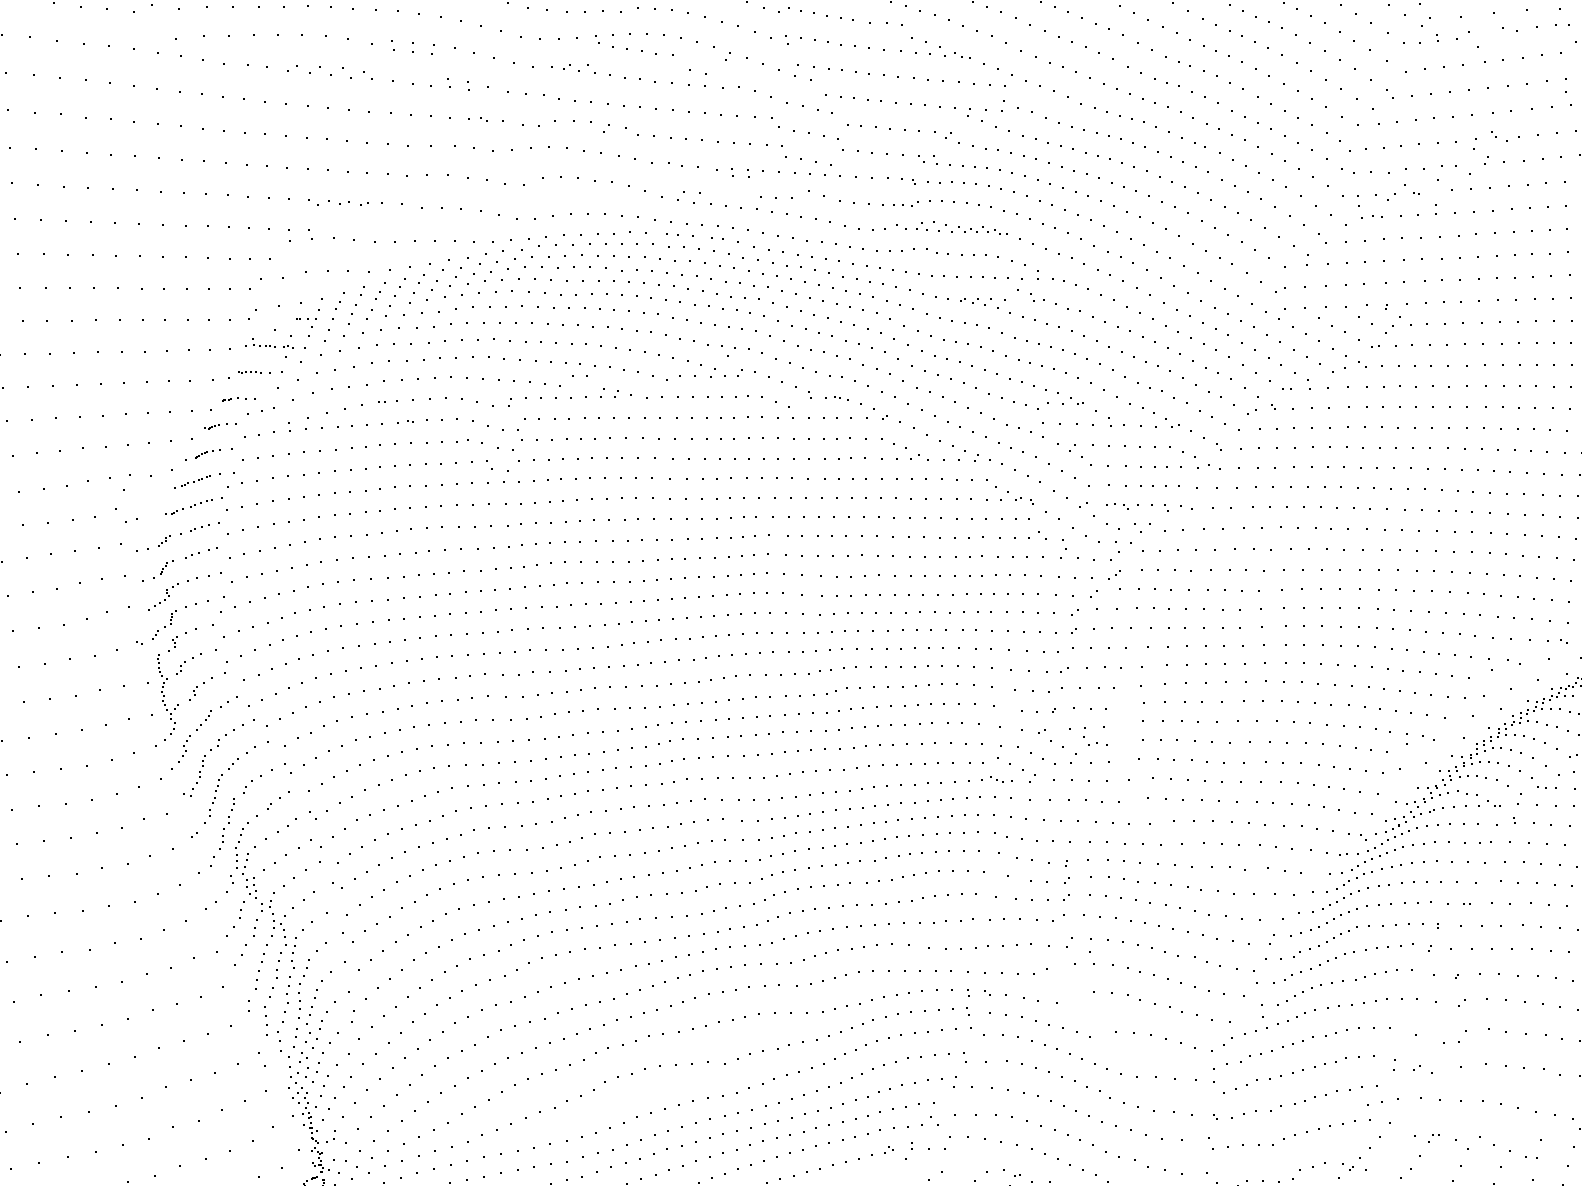
\includegraphics[width=.4\textwidth]{fig/bunny_grid_closeup.png}}
}
\caption{Closeup of the surface distribution of points on Bunny point cloud}
\label{fig:bunny_grid_closeup}
\end{figure}

The diagram on figure \ref{fig:pargrid_proj} shows the parallel projection of a square from camera image space onto a plane in three-dimensional space. $\vec{n}$ is the normal vector of the plane, $p_l$ the width and height (side length) of the square, and $x, y$ the corresponding side lengths of the projected square. It can be seen that the projected square takes on the shape of a parallelogram on the plane. This models the projection of scanner rays on a surface. The coordinate system is such that the scanner is placed at origin. Since only a small region of a locally planar surface is considered (compared to the field of view of the scanner), adjacent rays in azimuth and elevation direction are modeled as parallel. When the square is extended to form a square grid in the XY-plane, a parallelogram grid is formed on the plane in which all parallelograms have the same two side lengths and inner angles.

\begin{figure}[h]
\centering
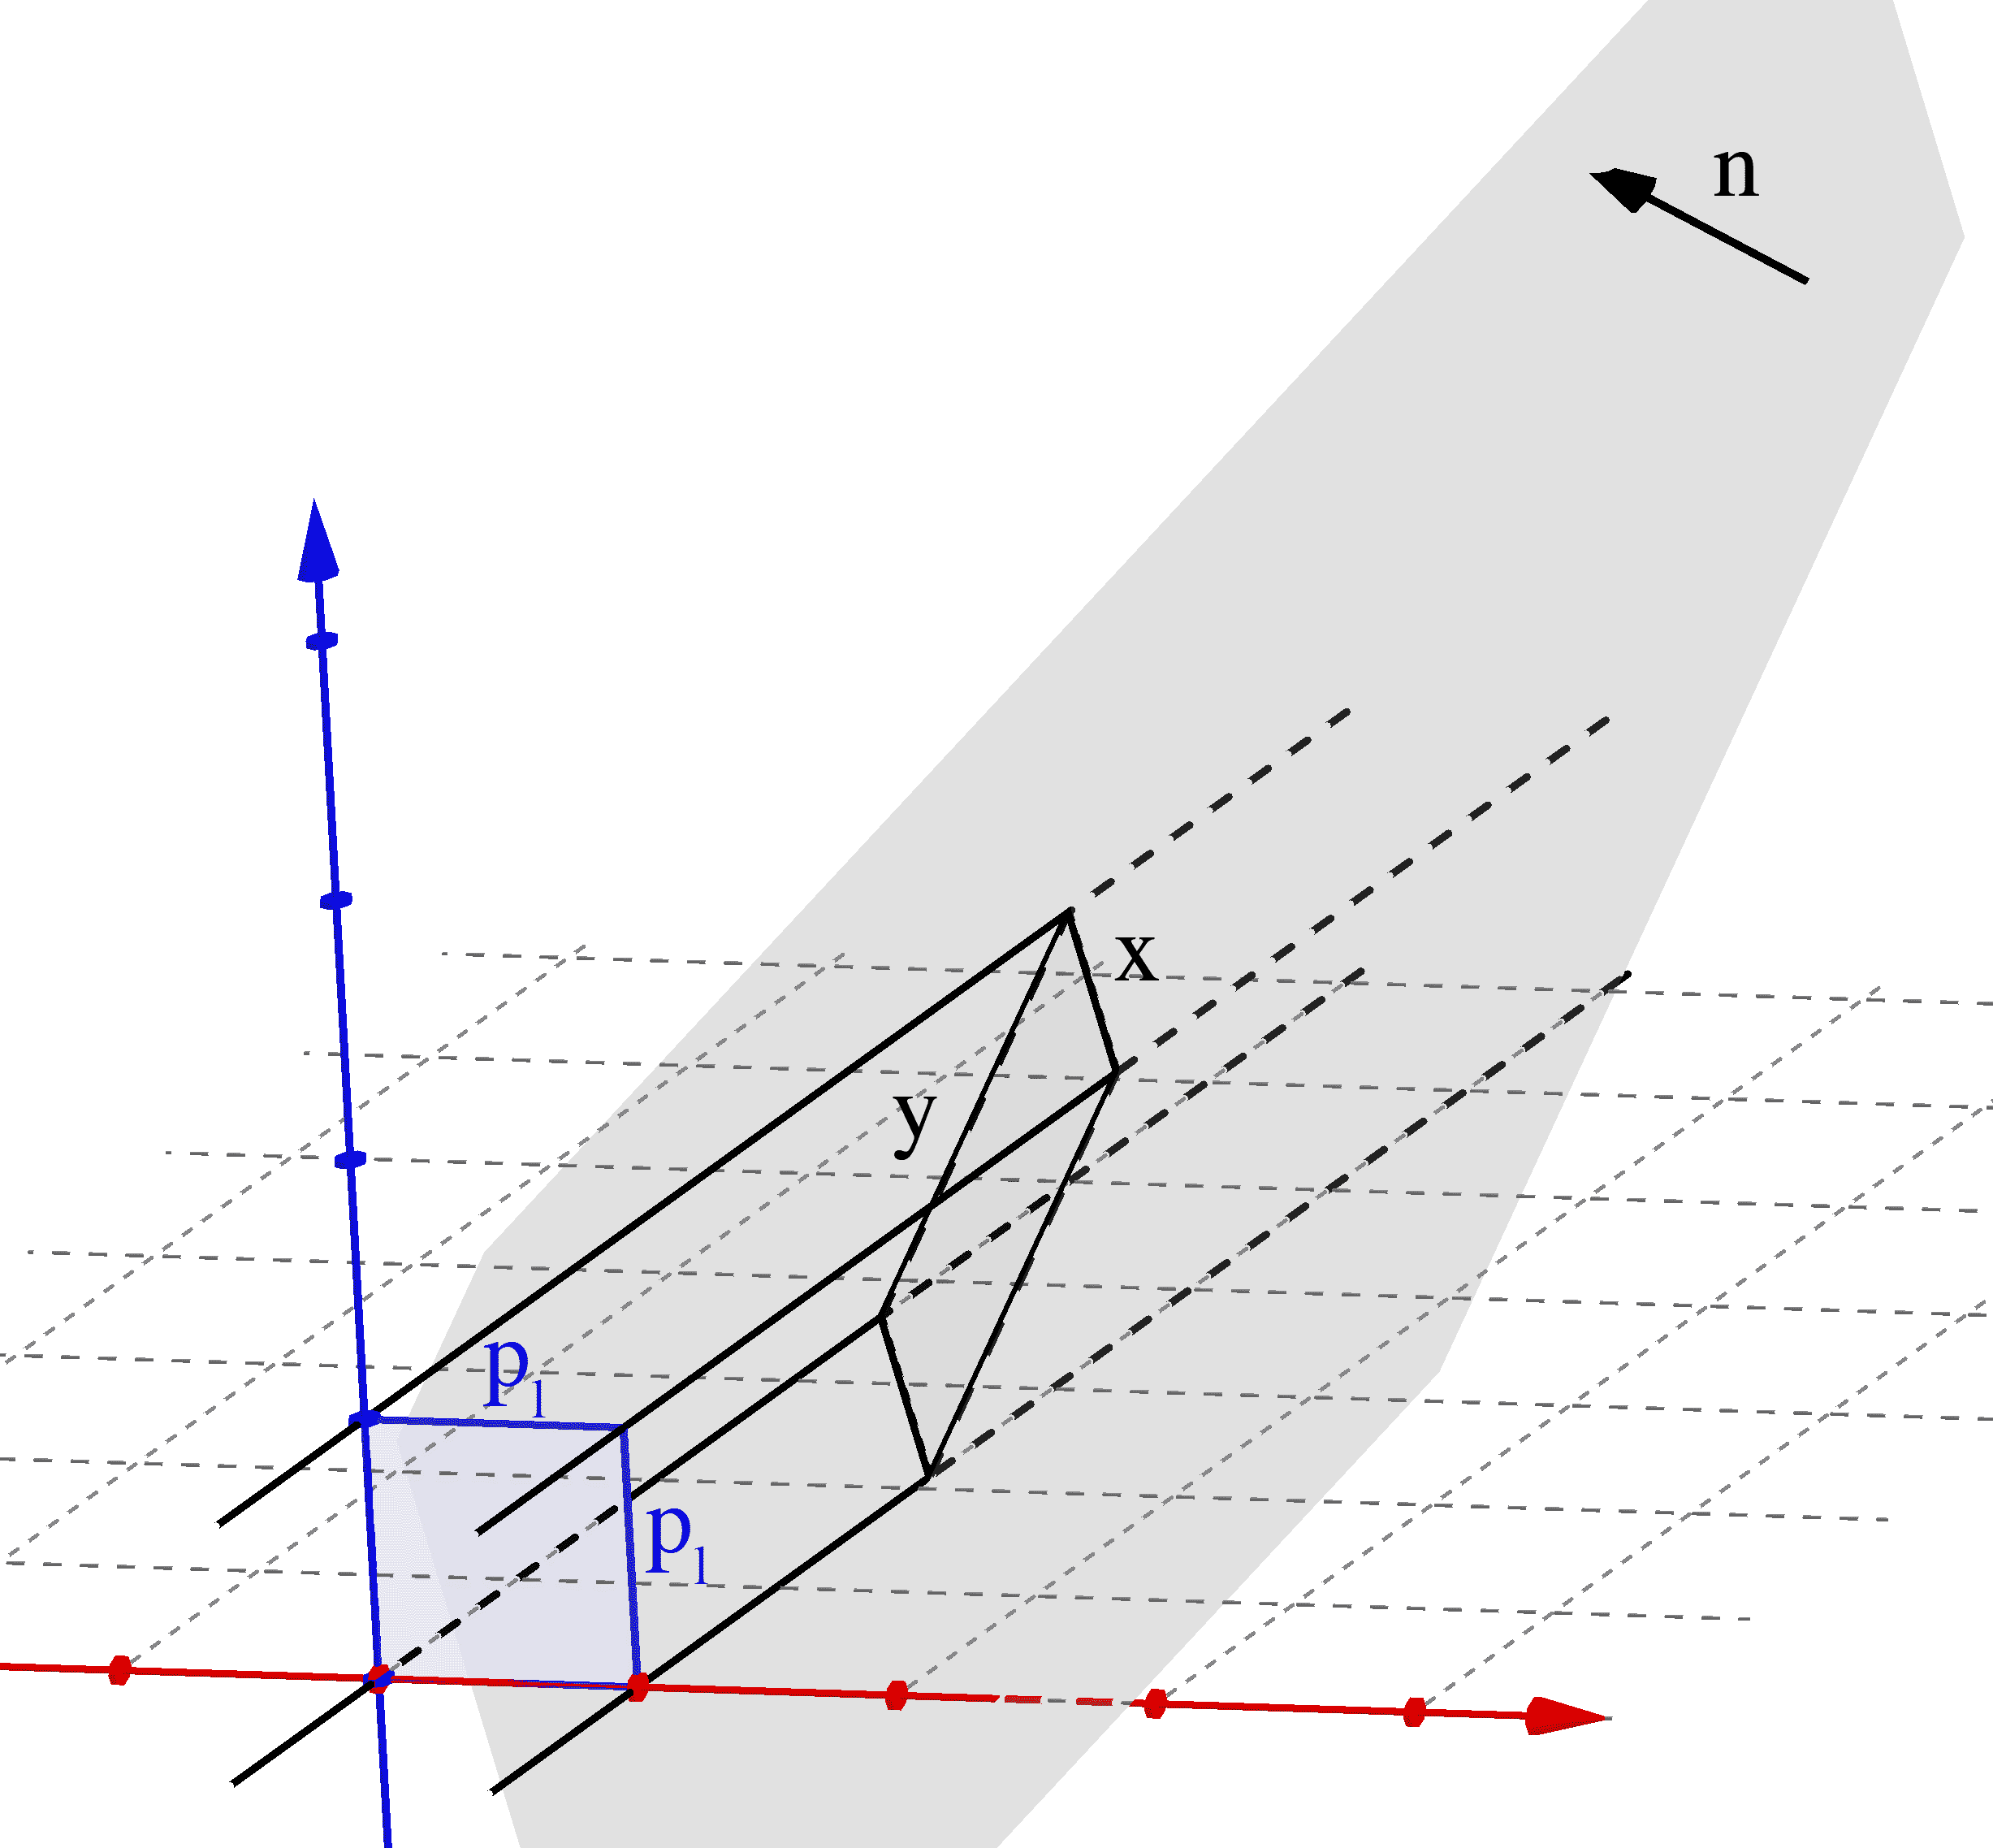
\includegraphics[width=.4\textwidth]{fig/pargrid_proj.png}
\caption{Parallel projection of square onto plane in space}
\label{fig:pargrid_proj}
\end{figure}

It can be seen on figure \ref{fig:par_grid_tilings} that several different parallelogram grids are possible for the same dispersion of points on the plane. The two grids in these examples have no sides in common. The projection of the camera square grid on the plane results in one of the possible parallel grids. When the plane is placed at a more oblique angle from the camera, it tends to be a grid with longer side lengths, such as the second on on the figure. It is not necessarily such that it includes the shortest possible parallelogram edge.

The ``parallelogram grid'' is described mathematically as a lattice in $\mathbb{R}^2$. The projections of $\vec{x} = \transpose{(p_l, 0)}$ and $\vec{y} = \transpose{(0, p_l)}$ from the camera image constitute one of the infinitely many possible bases for this lattice. \cite{Galb2012}

\begin{figure}[h]
\centering
\hspace*{\fill}%
\begin{subfigure}{.33\textwidth}
{
	\setlength{\fboxsep}{0pt}%
	\setlength{\fboxrule}{0.5pt}%
	\fbox{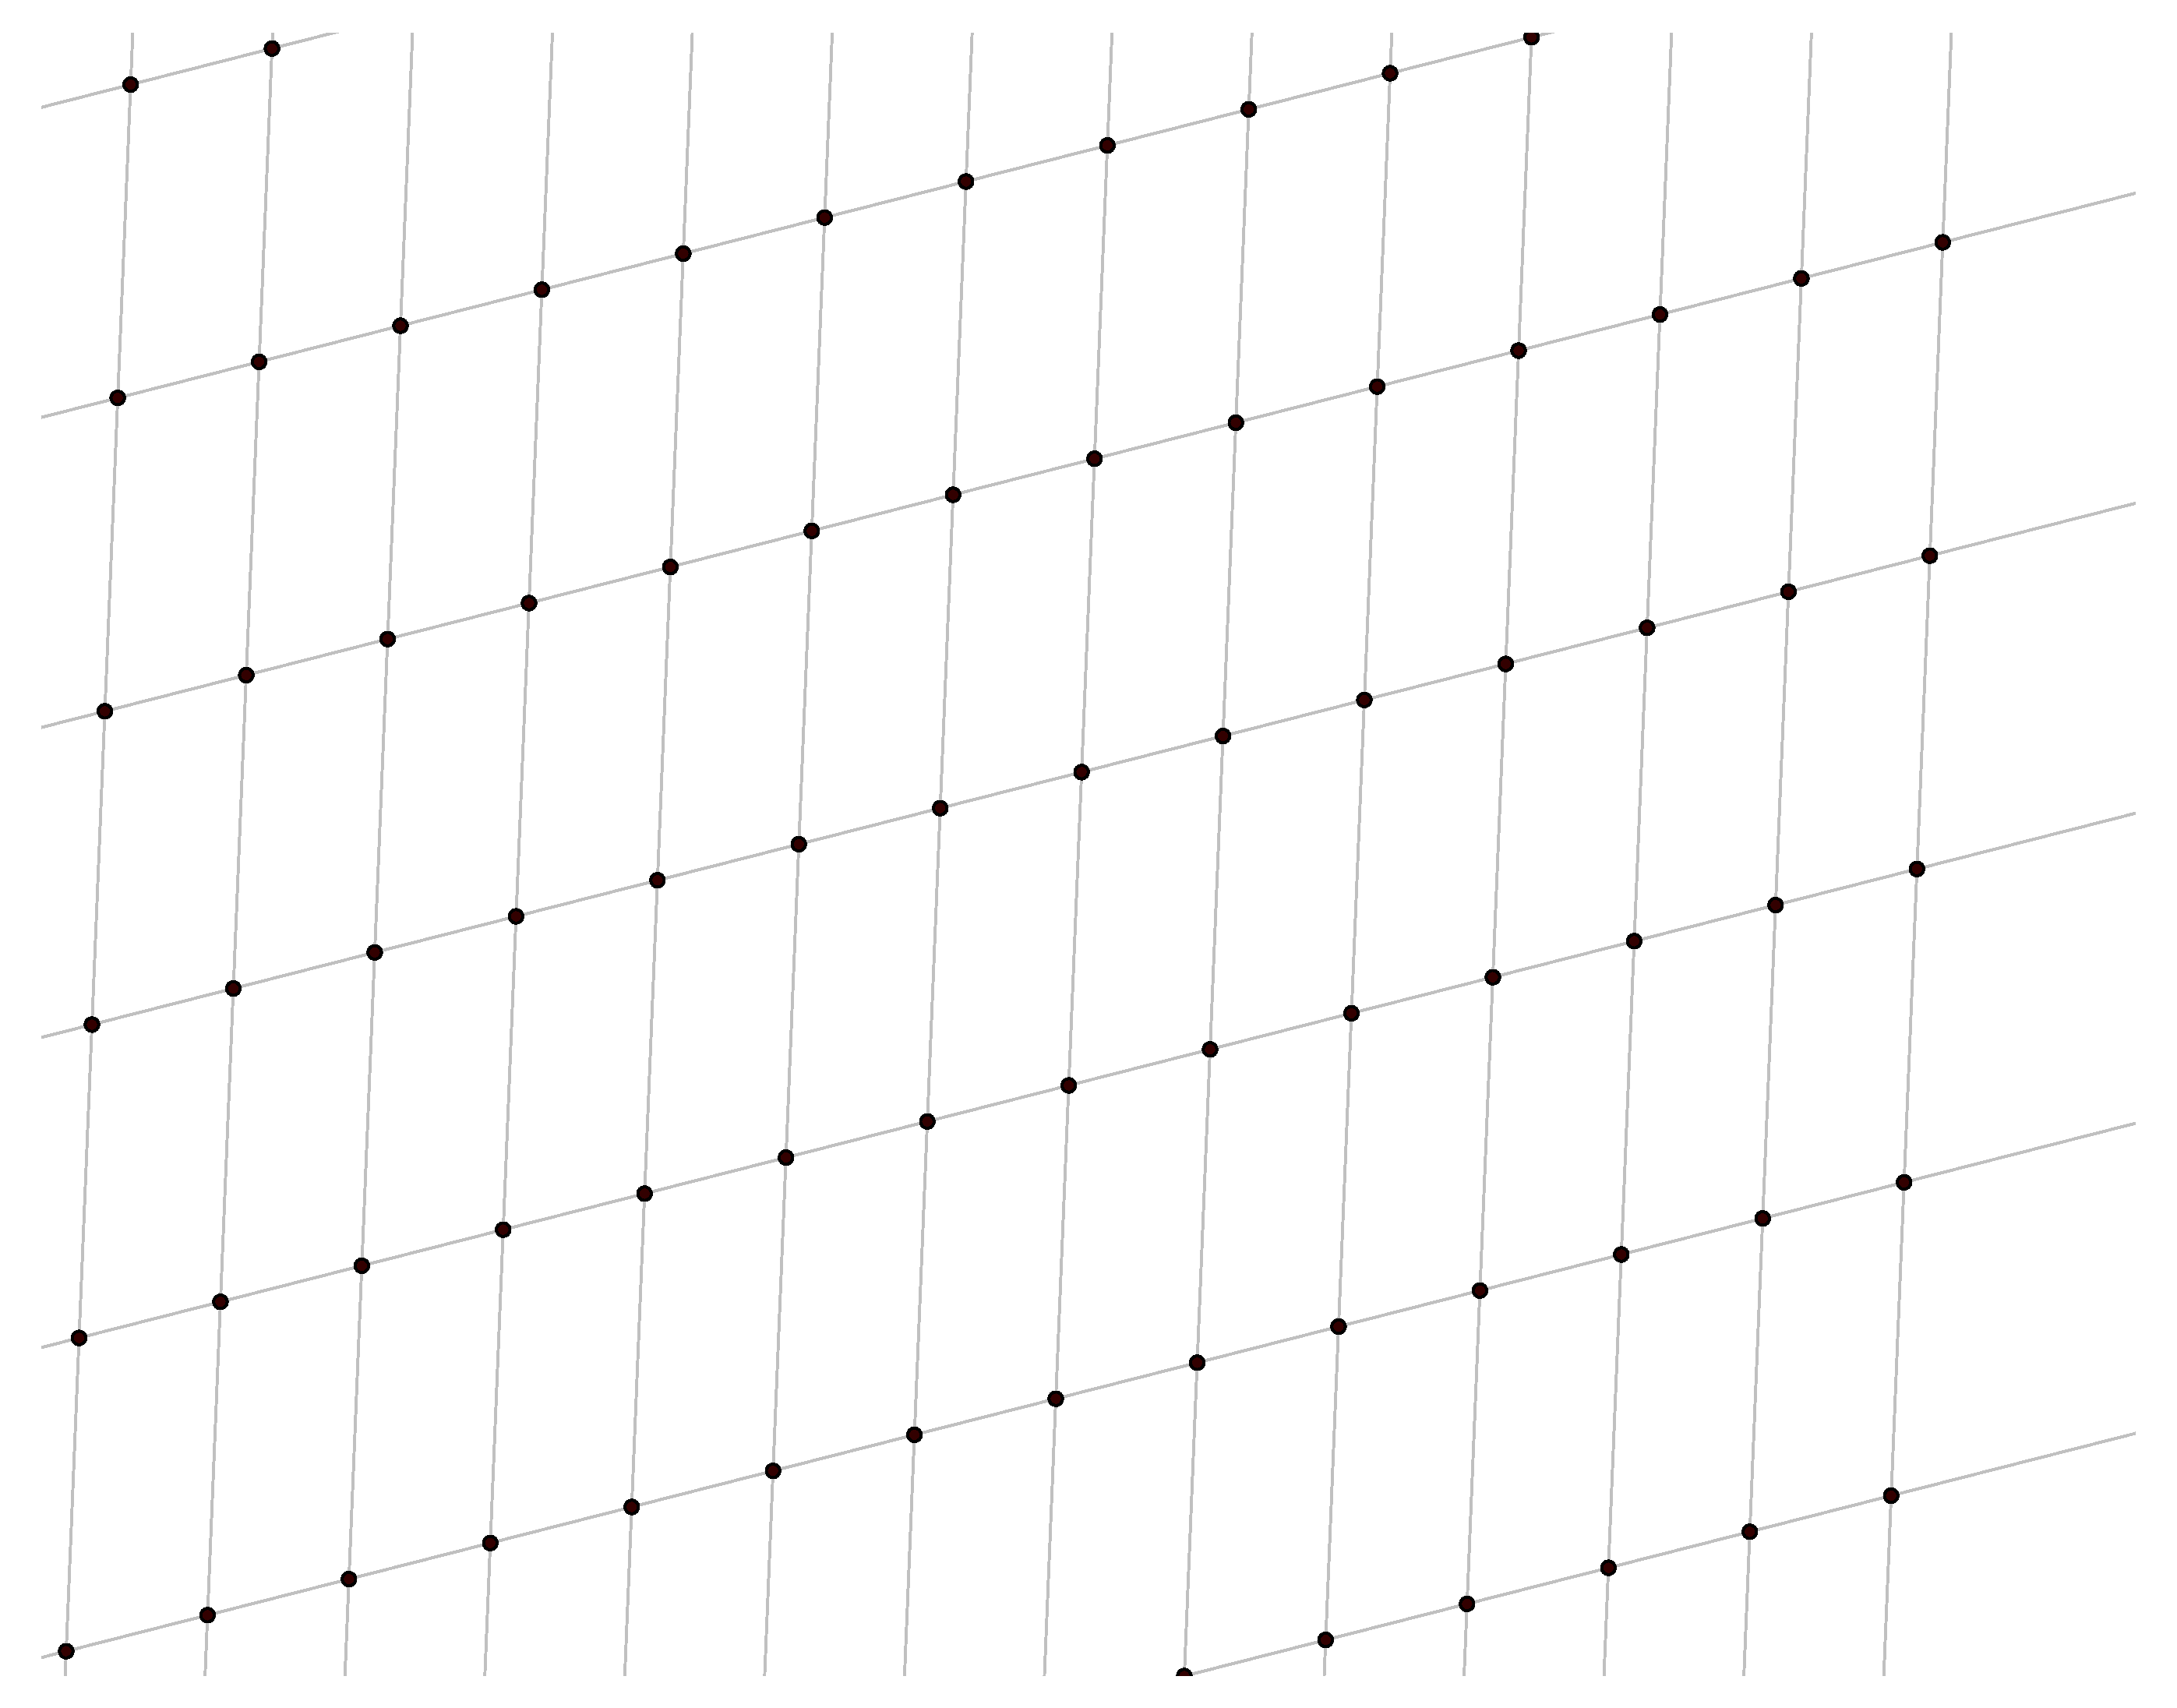
\includegraphics[trim=30 20 180 20, clip, width=\linewidth]{fig/pargrid1.pdf}}
}\end{subfigure}%
\hfill%
\begin{subfigure}{.33\textwidth}
{
	\setlength{\fboxsep}{0pt}%
	\setlength{\fboxrule}{0.5pt}%
	\fbox{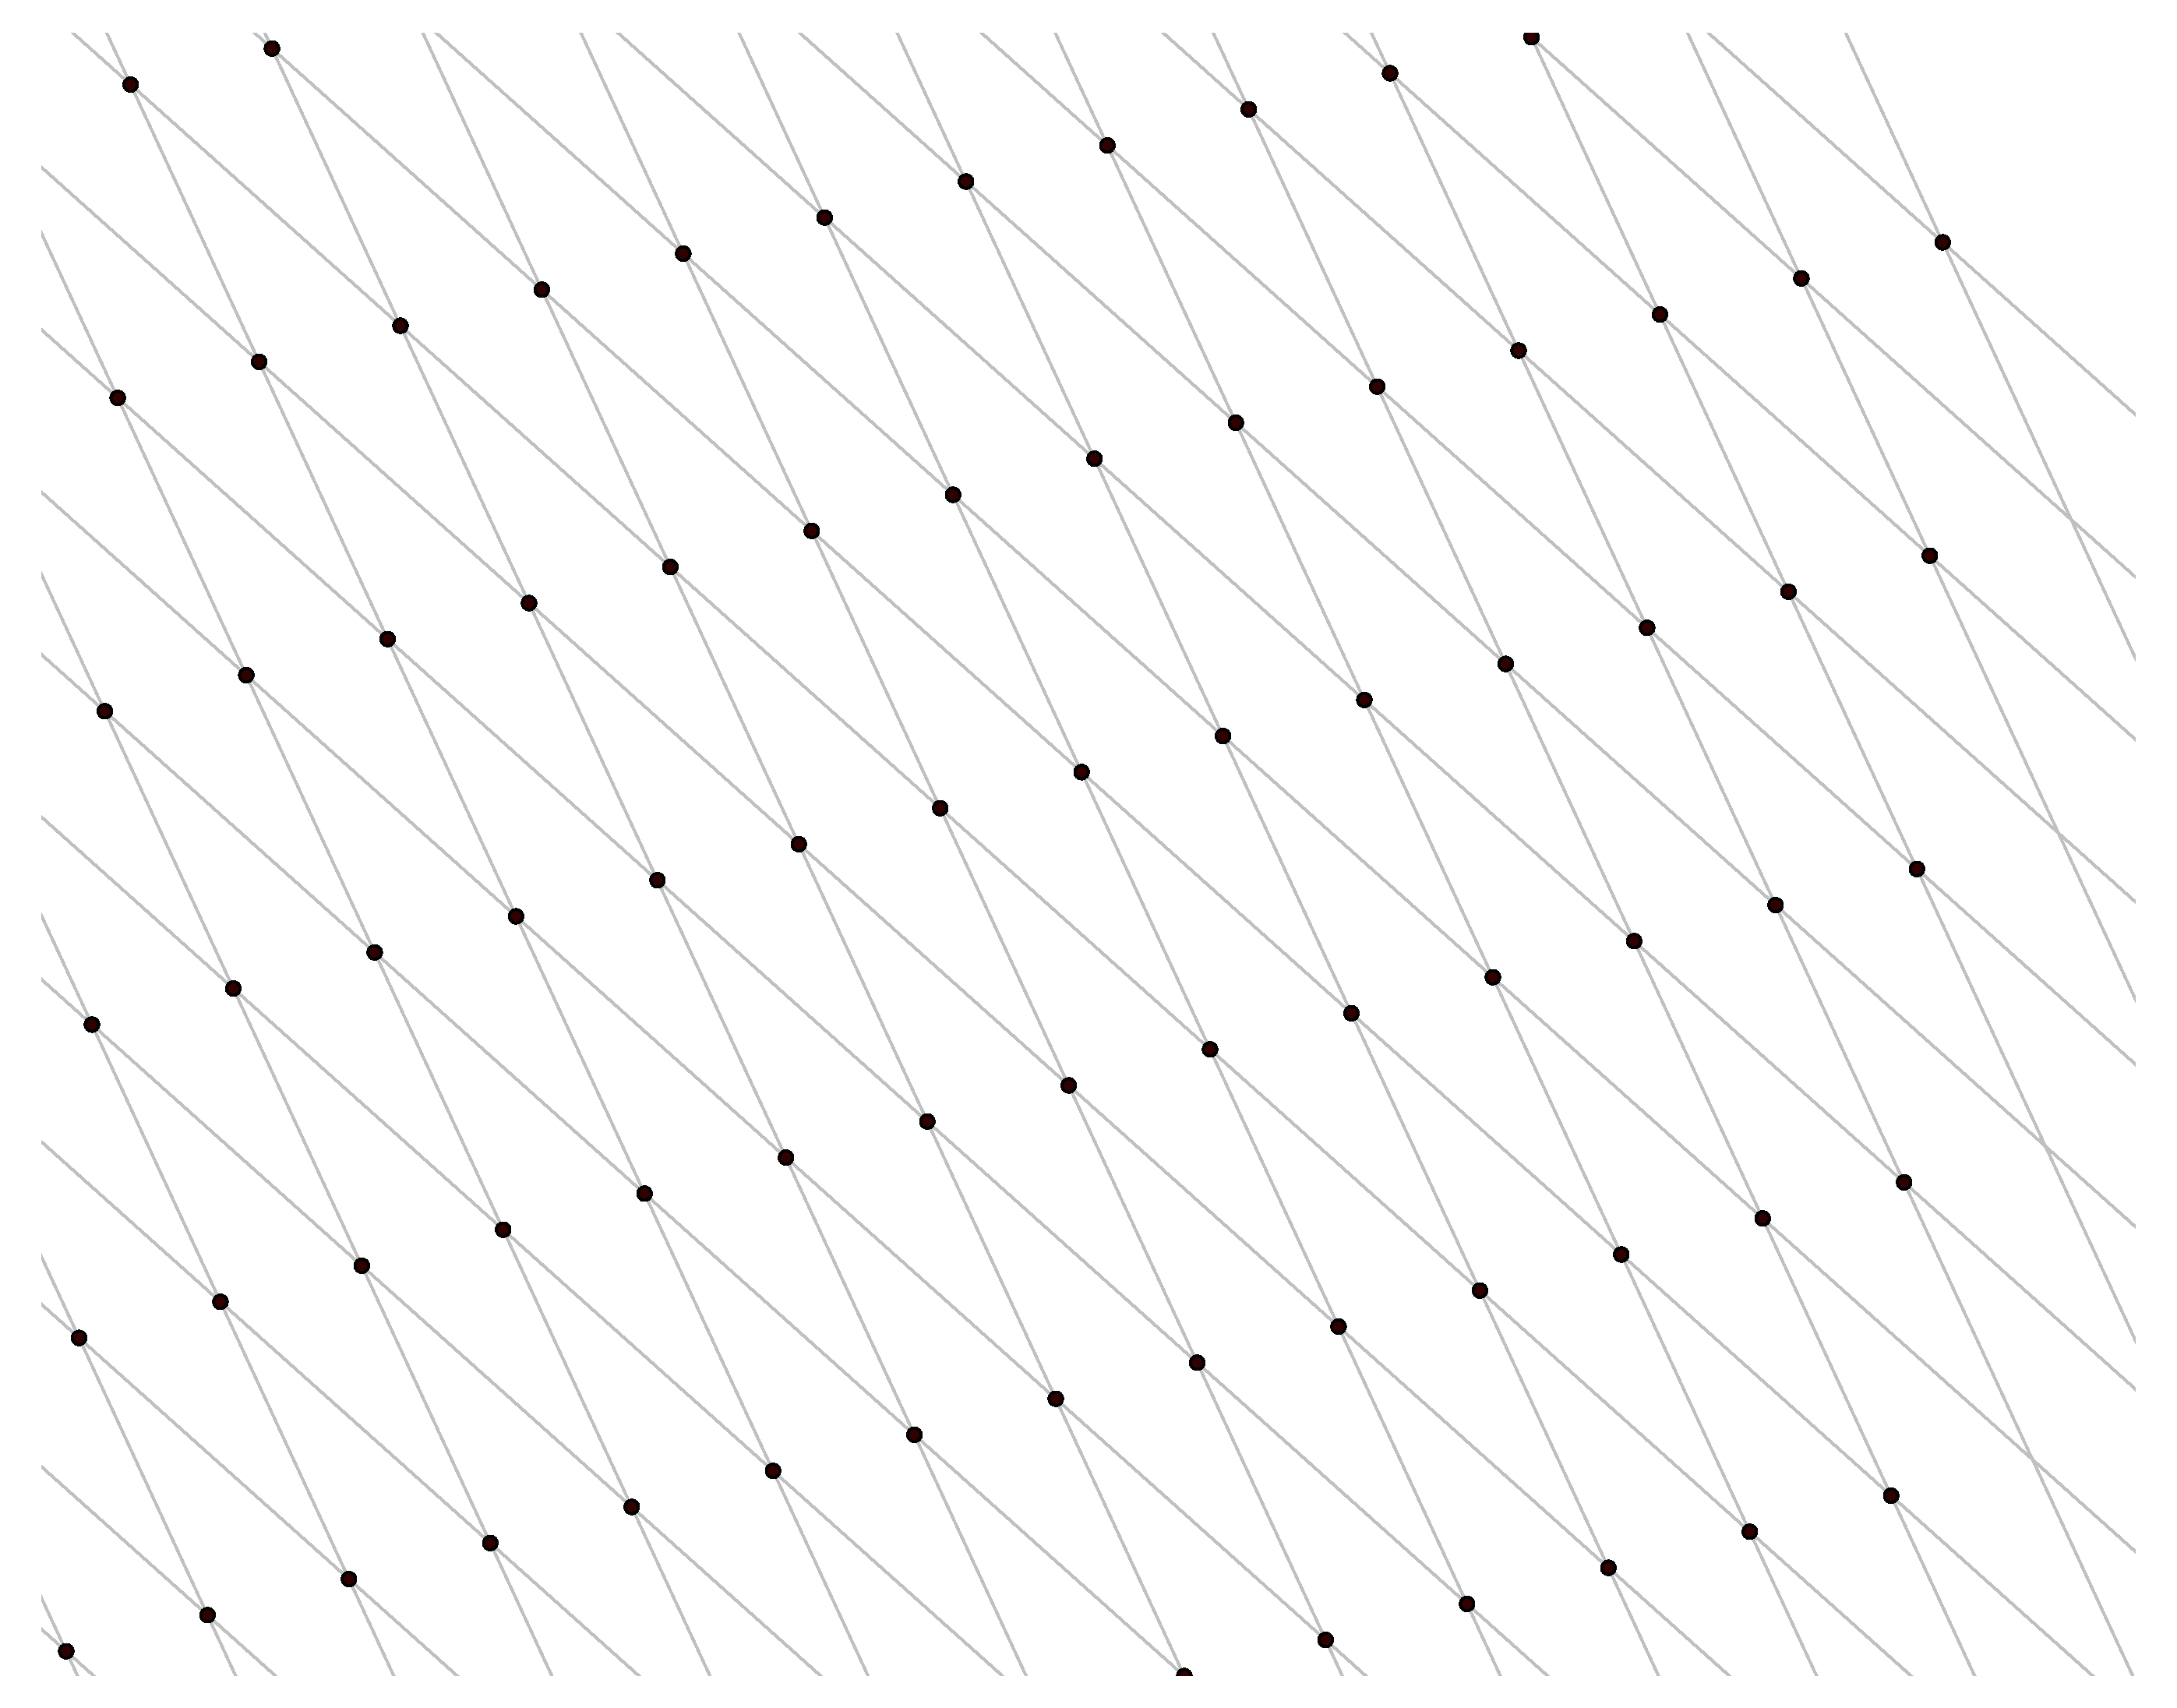
\includegraphics[trim=30 20 180 20, clip, width=\linewidth]{fig/pargrid2.pdf}}
}\end{subfigure}%
\hspace*{\fill}
\caption{Different parallelogram grids for same point dispersion}
\label{fig:par_grid_tilings}
\end{figure}


\subsection{Measures on grid}
The point density $\rho$ of the points in the parallelogram grid dispersion on the object surface, can be calculated as
\begin{equation}
\rho = \frac{| n_z |}{p^2_l}
\end{equation}

The shortest possible parallelogram side length $l_{\text{min}}$, for any parallelogram grid put on the points, can be estimated with the following formula, in function of $p_l$ and the normal vector $\vec{n}$ of a point $p \in P$. It is an estimate of the distance from $p$ to its closest neighbor. The expression gives correct values when $P$ is locally planar around $p$, and this plane is not too oblique.
\begin{equation} \label{eq:pargrid_lmin}
l_{\text{min}} \approx p_l \, \sqrt{1 + \frac{\min \left\{
	n^2_x, \,
	n^2_y, \,
	1 + 2 \, n_x \, n_y, \,
	1 - 2 \, n_x \, n_y
\right\} }{n^2_z}}
\end{equation}

A threshold condition for how oblique the surface may be is given by this formula
\begin{equation} \label{eq:pargrid_lmin_cond}
|n_z| > \cos \alpha \bigvee
\left[
\left|\frac{n_x}{n_y}\right| < \tan \beta
\bigwedge \left|\frac{n_y}{n_x}\right| < \tan \beta
\bigwedge \tan \left(\tfrac{\pi}{4} - \beta\right) < \left|\frac{n_x}{n_y}\right| < \tan \left(\tfrac{\pi}{4} + \beta \right)
\right]
\end{equation}
where the angles $\alpha$ and $\beta$ are adjusted to some constant. The lower these angles, the more restrictive the condition gets. $\alpha = 50\si{\degree}$ and $\beta = 10\si{\degree}$ were used for the experiments.

To check whether $P$ is locally planar around $p$, a curvature measure as described in \ref{sec:curvature} can be used. This is important since formula \ref{eq:pargrid_lmin} depends only on the normal vector, but on curved surfaces, the normal vectors gradually change direction. So on curved surfaces they reach any intermediate value, even when the nearest neighbor distances don't correspond to the predicted value from the formula.

The deduction and proofs for these formulea are given in appendix \ref{sec:proof_pargrid_measures}.



\subsubsection{Analysis}
Figure \ref{fig:lmin_plot} shows the value $l_{\text{min}}$, in function of the normal vector $\vec{n}$ of the plane. For the color scale a logarithmic scale is used. Blue and green correspond to lower values. The $x$ and $y$ axis of the plot correspond to $n_x$ and $n_y$, the third component is set to $n_z = \sqrt{1 - n^2_x - n^2_y}$. The plot is symmetric around the X and Y axis. The origin point $(0, 0)$ corresponds to $\vec{n} = \transpose{(0, 0, 1)}$, that is, the plane is perpendicular to the camera ray and has a square grid dispersion. Then $l_{\text{min}} = 1$, the side length of the square. For the points on either axis, the plane is turned on one direction only, resulting in a rectangular grid, where the shortest side remains $l_{\text{min}} = 1$. Around the border of the plot, the plane is nearly parallel to the camera rays. When $n_x \approx n_y$, the parallelograms take on a rhombus shape, similar to the second grid shown on figure \ref{fig:par_grid_tilings}. The shortest edge becomes the projection of the squares' diagonal with length $\sqrt{2}$, whereas the projection of its sides results in longer edges.

\begin{figure}[p]
\centering
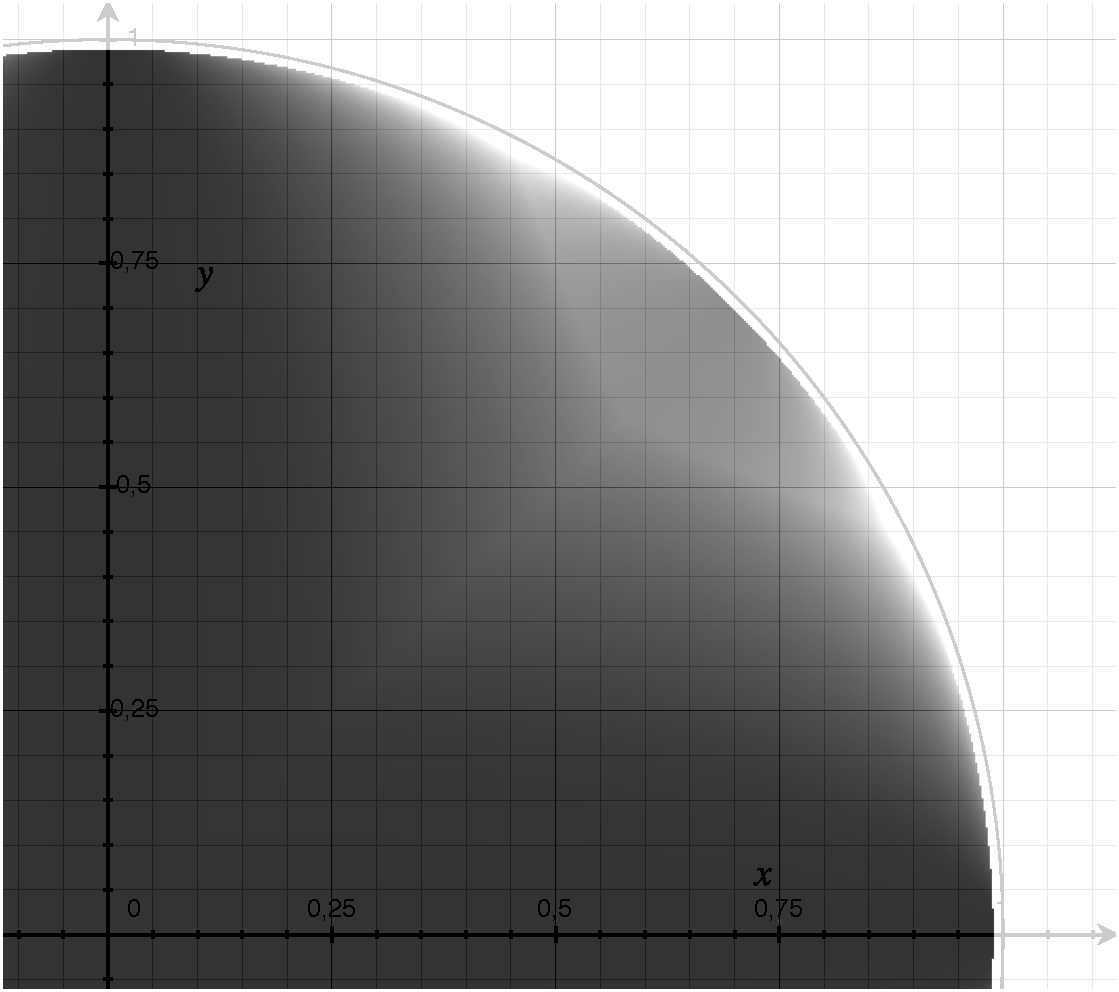
\includegraphics[width=.4\textwidth]{fig/lmin_plot.pdf}
\caption{Plot of $l_{\text{min}}$ for $\vec{n} = \transpose{(x, y, \sqrt{1 - x^2 - y^2})}$ and $p_l = 1$}
\label{fig:lmin_plot}
\end{figure}


\subsubsection{Verification}
The first (left-side) histogram on figure \ref{fig:relief_nn_hist} was generated by recording for each point $p \in P$ on a point cloud, the distance $d$ to its closest neighbor. (That is, the point $p' \in P$ such that $p' \neq p$ and $\| p - p' \|$ is minimal.) The point cloud $P$ used is a ``relief'' model as described before in section \ref{sec:relief}, projected without occlusion using a parallel projection camera with $p_l = 0.01$.

Two clusters form around $0.01$ for parts of the surface that are near-parallel to the camera rays, and around $0.0115$, where the surface is more oblique in both directions. Since the surface is not everywhere locally planar the histogram does not form sharp spikes.

For the second histogram the values $l_{\text{min}}$ are instead recorded using the normal vectors of the points $p \in P$, and with fixed $p_l = 0.01$. This histogram is generated solely by evaluating the formula \ref{eq:pargrid_lmin}, without looking at the coordinates of the points, or doing a closest neighbor search in $P$.

\begin{figure}[H]
\centering
\begin{subfigure}{.5\textwidth}
	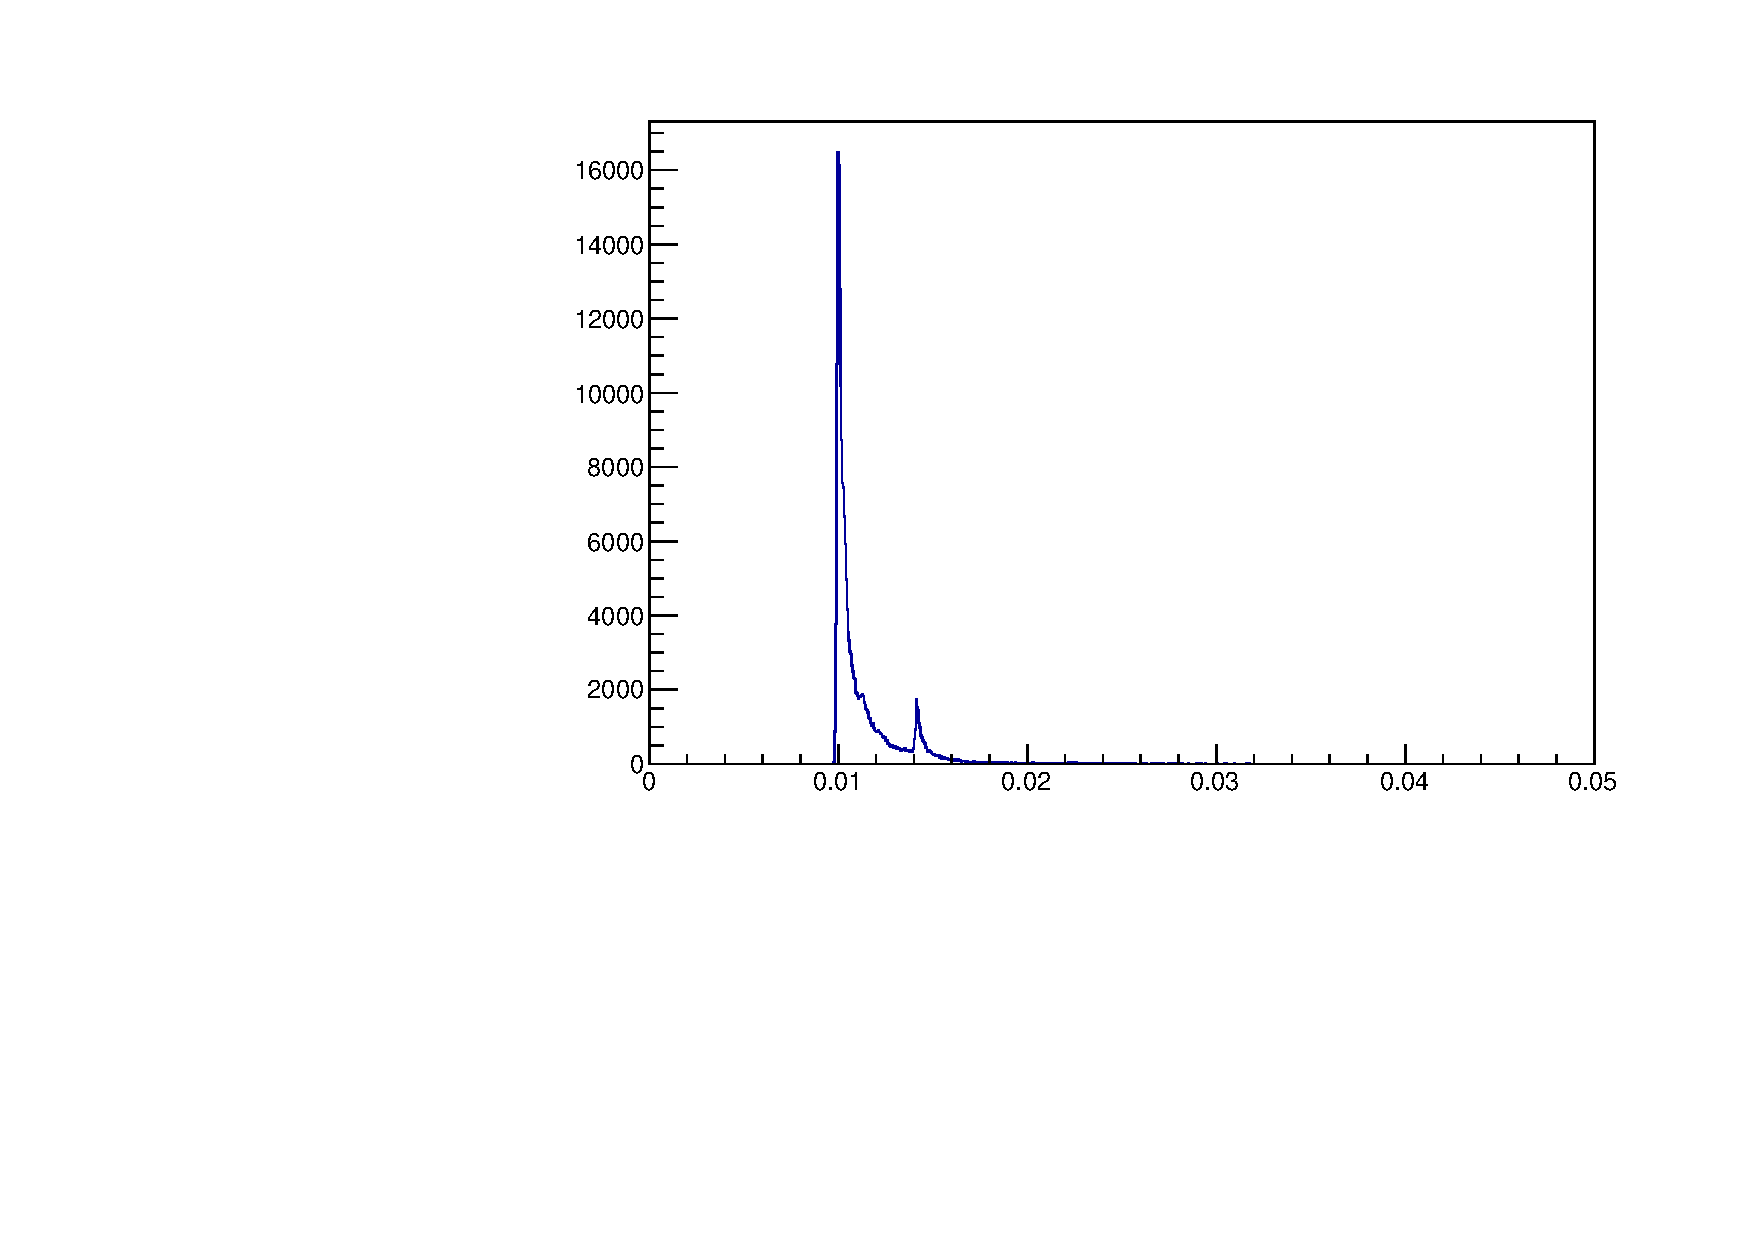
\includegraphics[width=\linewidth]{fig/nn.pdf}
	\caption{Closest neighbor distances on $P$}
\end{subfigure}%
\begin{subfigure}{.5\textwidth}
	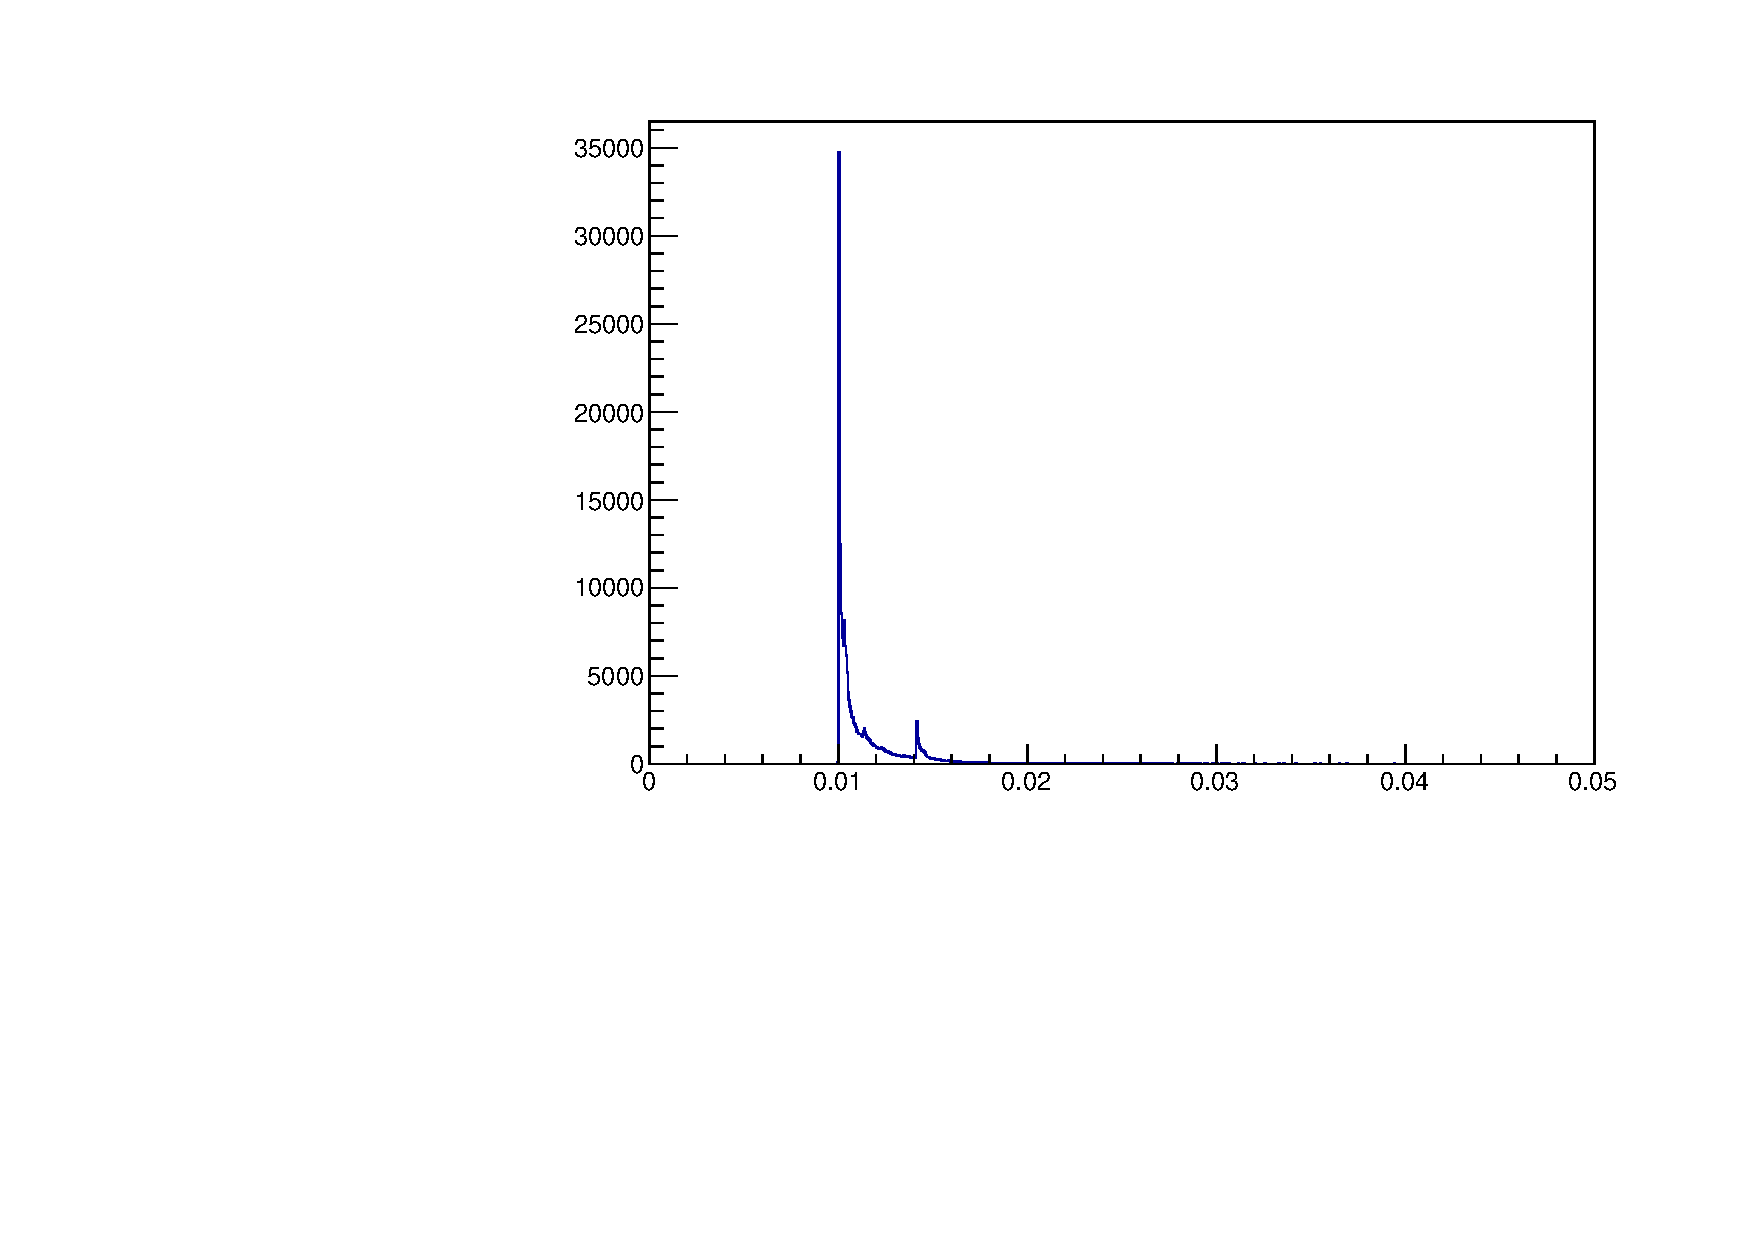
\includegraphics[width=\linewidth]{fig/nn_lmin.pdf}
	\caption{Values $l_{\text{min}}(\vec{n})$ on $P$}
\end{subfigure}	
\caption{Comparison of measured closest neighbor distances and $l_\text{min}$ values on relief point cloud.}
\label{fig:relief_nn_hist}
\end{figure}

A similar distribution can be observed on both histograms. The spike at $0.01$ occurs because the camera is placed such that the majority of the surface is approximatively perpendicular to the rays. This confirms the correctness of the formula for $l_{\text{min}}$ for the parallelogram dispersion generated by parallel projection. The similarity of these two histograms also allows for estimation of $p_l$, even when it is not a mode.
 

\subsubsection{Usage on real point cloud scan}
Figure \ref{fig:ddp_nn_hist} shows the same two histograms, using the ``dessus-de-porte'' scan for $P$ instead of an artificial relief point cloud. The points whose normal vectors fail the threshold condition \ref{eq:pargrid_lmin_cond} or whose curvature is too high are removed prior to taking the histogram.

Some similarity can still be seen, notably the two spikes near $d = 0.0024$ and $d = 0.0034$. Many factors cause the discrepancy between the two histograms:
\begin{itemize}
\item There is some error in the points' positions, which becomes significant in the order of magnitude of nearest neighbor distances. They do not lie exactly on the object surfaces, and do not form a perfect lattice on the surfaces.
\item The scanner does not form exactly the parallelogram lattices as predicted.
\item The scanner rays are not exactly parallel throughout the point cloud.
\item The surface is nowhere completely planar.
\item As explained, the formula \ref{eq:pargrid_lmin} is only correct in a subset of the cases, even when the condition \ref{eq:pargrid_lmin_cond} is applied.
\item The normal vectors are not completely accurate.
\end{itemize}

\begin{figure}[H]
\centering
\begin{subfigure}{.5\textwidth}
	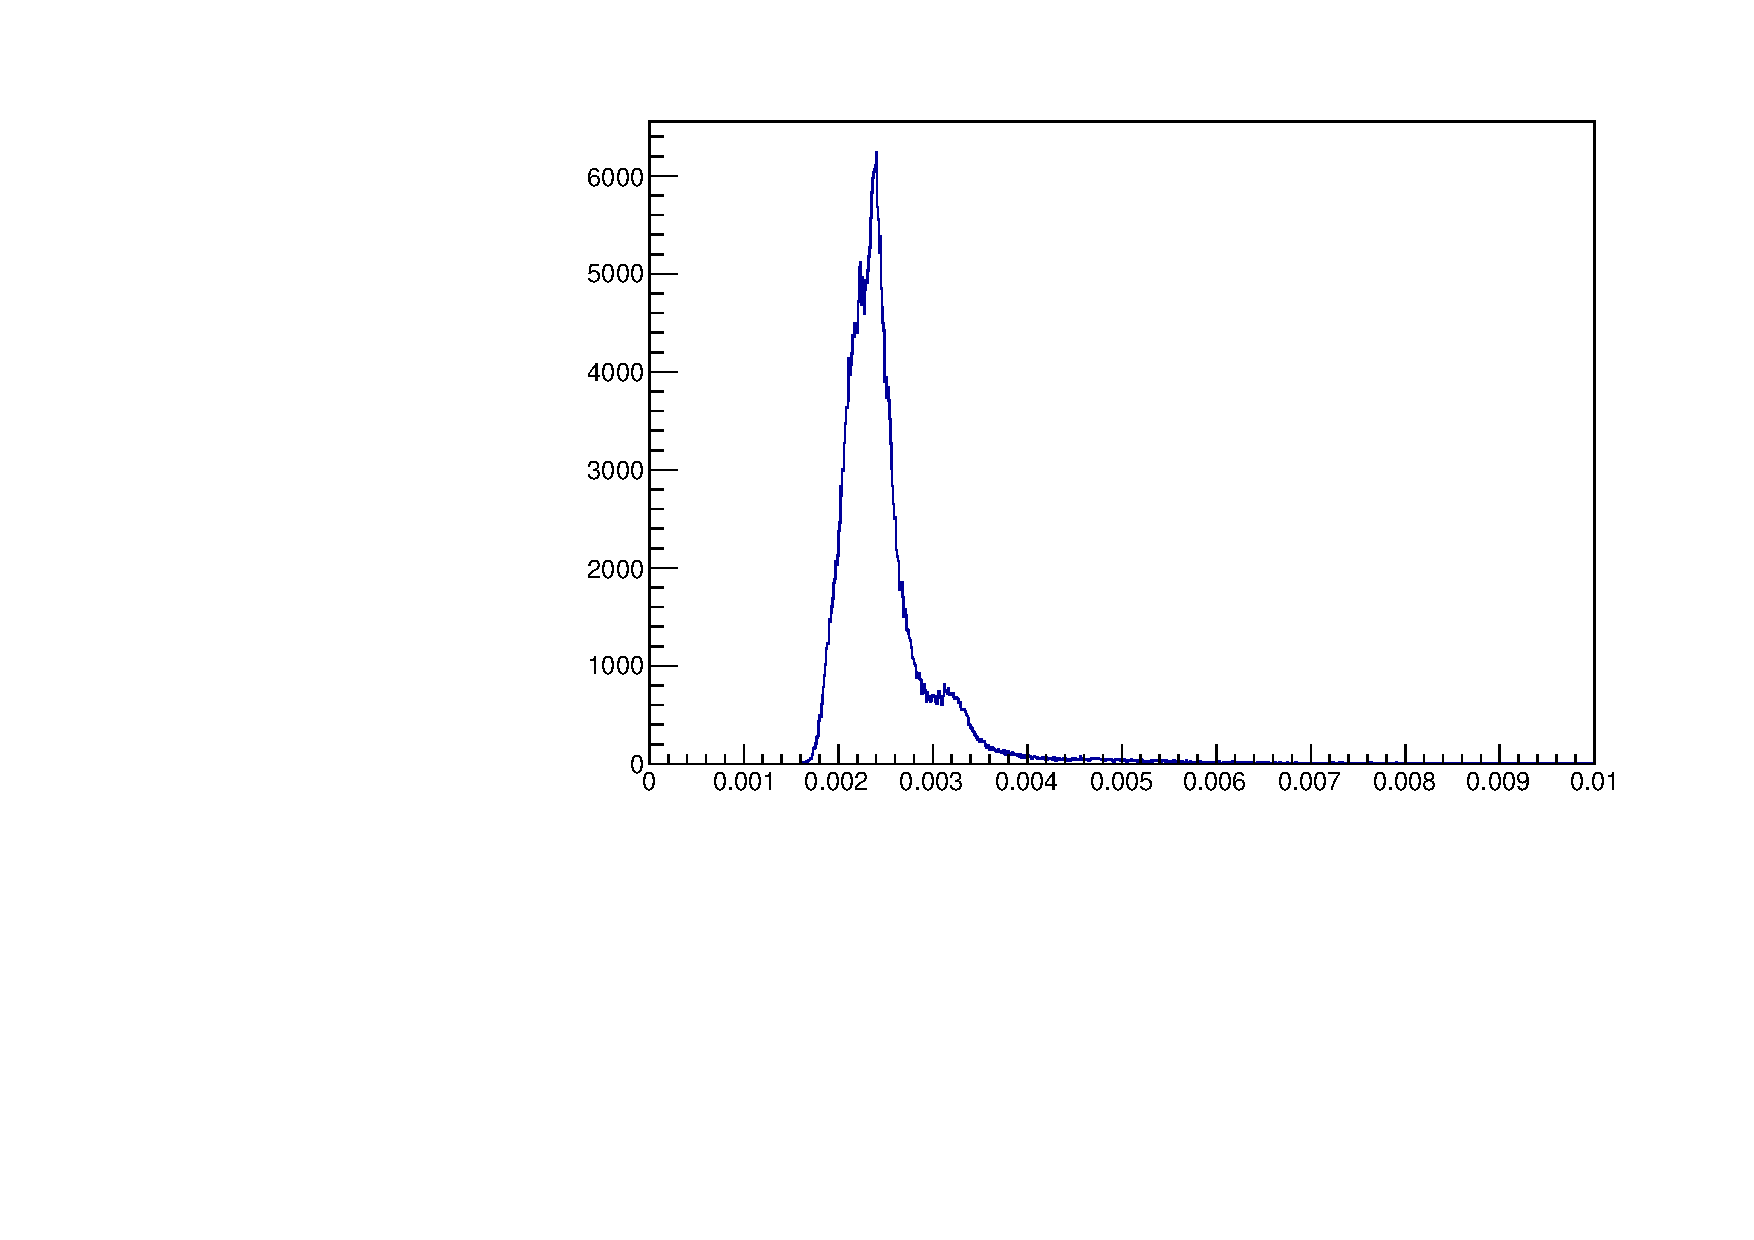
\includegraphics[width=\linewidth]{fig/ddp_nn.pdf}
	\caption{Closest neighbor distances on $P$}
\end{subfigure}%
\begin{subfigure}{.5\textwidth}
	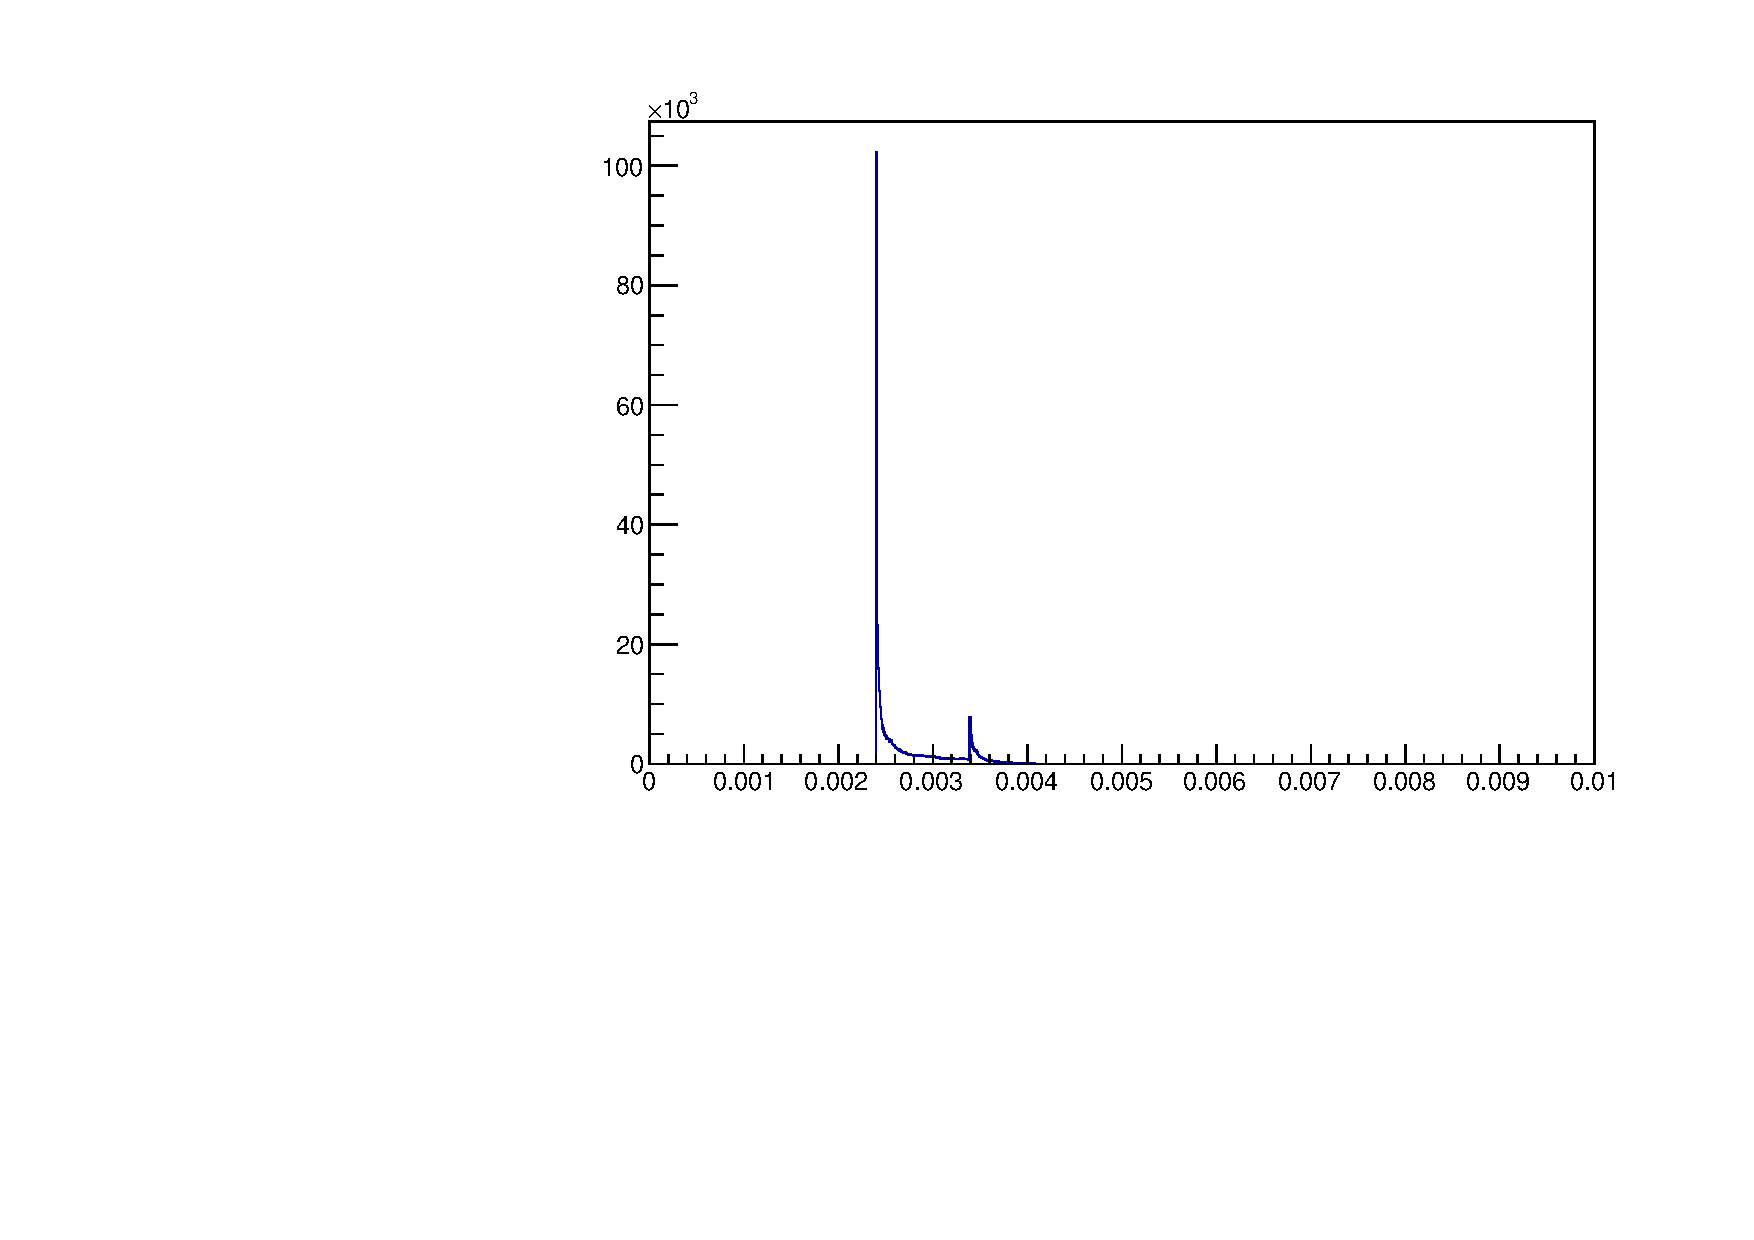
\includegraphics[width=\linewidth]{fig/ddp_nn_lmin.pdf}
	\caption{Values $l_{\text{min}}(\vec{n})$ on $P$}
\end{subfigure}	
\caption{Comparison of measured closest neighbor distances and $l_\text{min}$ values on ``dessus-de-porte'' scan.}
\label{fig:ddp_nn_hist}
\end{figure}



\subsection{Estimation of projection parameters} \label{sec:estimate_proj_par}
If the point cloud $P$ was generated using a parallel projection camera where the graduation in the $x$ and $y$ directions on the image planes is the same, a value $p_l$ exists for the point cloud. This remains true by approximation for small extracts of large 3D scans. In the following the assumption is made that a constant value $p_l$ exists for the entire point cloud.

As shown before, using the properties of the parallelogram grid dispersion and formula \ref{eq:pargrid_lmin}, $p_l$ can be estimated by analyzing the points of the point clouds and their normal vectors. The formula is such that $l_{\text{min}}$ is proportional to $p_l$, and the proportionality constant $m(\vec{n}) = \min \left\{ \cdots \right\}$ is a function of $\vec{n}$. In this formula the coordinate system is such that the camera is at origin, so that a normal vector $\vec{n} = \transpose{(0, 0, 1)}$ points towards it. When $P$ is set in a different coordinate system but the camera pose in it is known, the necessary transformation must be applied. As stated in section \ref{sec:range_image} it is supposed to be the case for range images point clouds.

Assuming that the parallelogram grid covers the entire surface and that the surface is locally planar, $l_{\text{min}}(p)$ can be computed at each point by measuring the distance to the closest neighbor in the point cloud.

A way to estimate $p_l$ is to record $\frac{l_{\text{min}}(p)}{m(\vec{n})}$ for each point and take the median value. The histogram is such that there is one large spike at the correct value $p_l$, and some outliers far off. For point clouds with a high number of points, this estimation remains stable when samples are recorded only for a random subset of the points.


\newpage

\section{Own distance histogram}
Let $P$ and $Q$ be two perfectly aligned point clouds with identical surfaces, but with different point dispersions. They can differ as described in \ref{sec:registration_robostness}. $P$ is called the \emph{model}, and the points $q \in Q$ the \emph{samples}. For each sample $q \in Q$, the closest point $p \in P$ is chosen, and the distance $\|p - q\|$ is recorded. The histogram of these distances will be called the \gls{odh}. The points $p$ are chosen by the closest point criterion, without additional constraints at first.

In this section the shape of this histogram will be analyzed, and in the next section it will be compared to the \acrfull{cdh}, for which $P$ and $Q$ are no longer identical or perfectly aligned.

By replacing the samples $q \in Q$ with a random variable $\textbf{Q}$ with a given probability distribution, the \gls{odh} can be idealized into a probability density function of the closest point distance, free of noise resulting from the sparse set of samples.

In the following, $Q$ will be taken to have a much higher point density than $P$. When the number of samples becomes infinite, the histogram converges towards the ideal probability density function. The results will later be applied to devise a method for registering high resolution with low resolution point clouds.

When used on two exact same copies of the same point clouds that are perfectly aligned, all measured distances are $0$, and so the histogram consists only of one spike.

When $P$ is artificial and its surface shape is known, $Q$ is constructed by taking a large number of points on that same surface.

\subsection{Plane with random dispersion}
Figure \ref{fig:plane_rand_d30000} shows an \gls{odh}, where $P$ and $Q$ represent a single plane, and the points $p \in P$ are randomly dispersed onto it with an uniform density $\rho(P) = 30000$. For each sample $q$ the distance $d(q, P)$ to the closest point in $P$ is measured. Randomly dispersed means that the $x$ and the $y$ coordinate of each point are chosen randomly and independently, with a uniform distribution in a fixed interval.

Since $P$ and $Q$ are perfectly aligned, in this situation all distances are measured on the two-dimensional plane.

\begin{figure}[H]
\centering
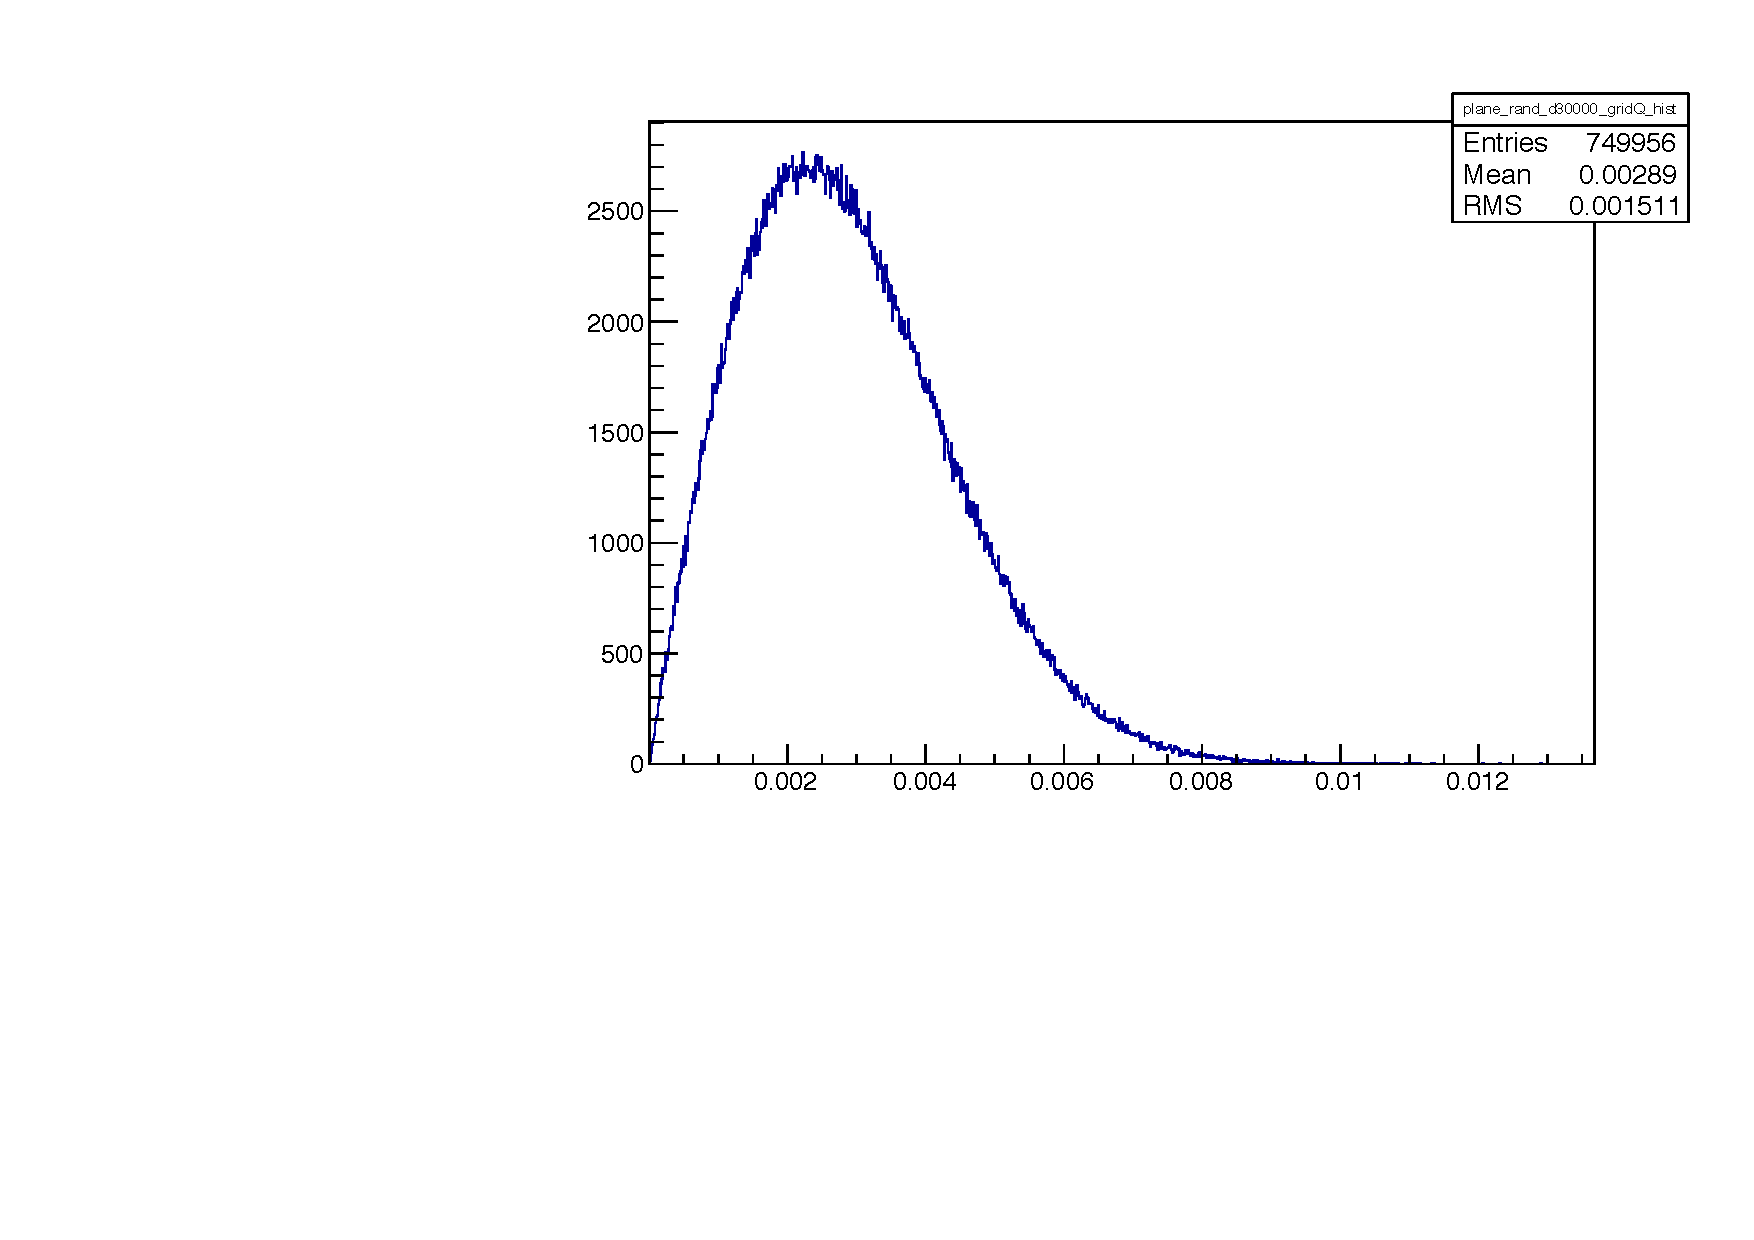
\includegraphics[width=.6\textwidth]{fig/plane_rand_d30000_gridQ.pdf}
\caption{Own distance histogram for plane $P$ with random point distribution}
\label{fig:plane_rand_d30000}
\end{figure}

Unless two points coincide, the probability at $d = 0$ is zero. It then increases, because the probability that a disk with radius $d$ around a sample point $q$ contains at least one $p \in P$ gets larger proportionally to the disk's area. But that disk must increase in radius to contain more than one point, otherwise the closest distance is the distance to the first, closer point inside the disk, and not its radius. This intuitively explains the global shape of the histogram.

The underlying probability density function $f_R$ of the random closest point distance $R$ from any point $q$ is the exponential function
\begin{equation}
f_R(r) = 2 \pi \rho(P) \, r \, e^{-\pi \rho(P) \, r^2}
\end{equation}
This formula is proven in appendix \ref{sec:proof_rand_disp_plane}. A plot is shown in figure \ref{fig:plane_rand_d}, for $\rho(P) = 30000$. It can be seen that the probability density function takes on the same shape as the histogram. By solving $\frac{\diffd}{\diffd r} f_R(r) = 0$, one obtains that the probability density function reaches its maximum at
\begin{equation}
r_{\text{mode}} = \frac{1}{\sqrt{2 \pi} \sqrt{\rho(P)}}
\end{equation}

The mean $\bar{r}$ value for the closest point distance is obtained using the integral
\begin{equation}
\bar{r} = \int_{0}^{\infty} r \, f_R(r) \, \diffd r = \frac{1}{2 \sqrt{\rho(P)}}
\end{equation}

\begin{figure}[p]
\centering
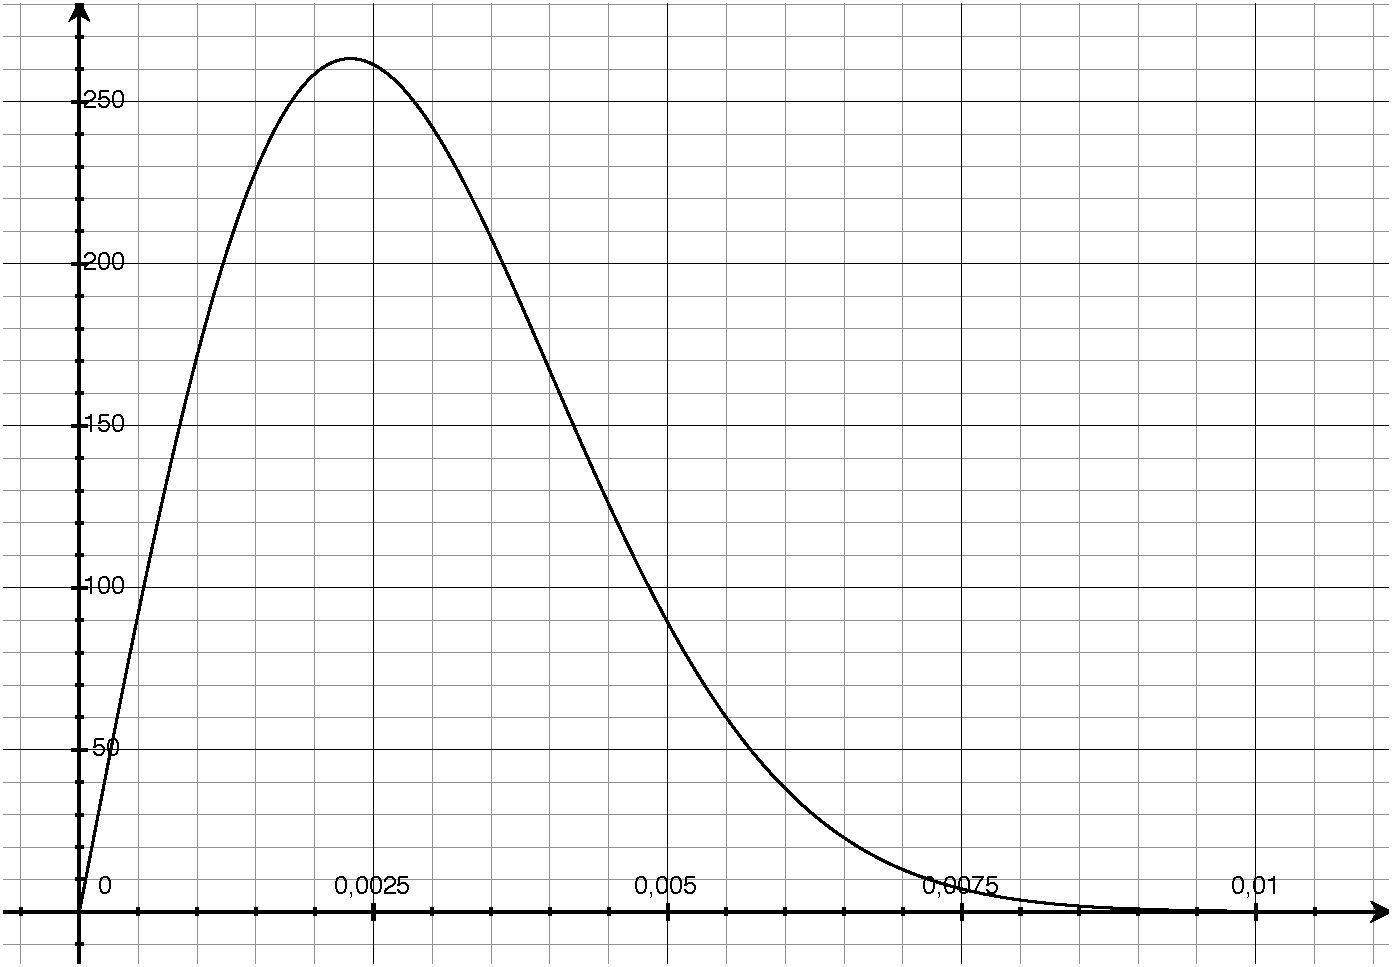
\includegraphics[width=.5\textwidth]{fig/plane_rand_d.pdf}
\caption{Probability density function of closest point distance, for plane $P$ with randomly dispersed points}
\label{fig:plane_rand_d}
\end{figure}

This random points dispersion represents the most general case, where no information about the dispersion of sample points on the surfaces is known. 



\subsection{Dispersion of sample points} \label{sec:disp_sample_pts}
In order to obtain a histogram that closely resembles the theoretical probability density function, the dispersion of the sample points $q \in Q$ should be such that its density is much higher than that of the model points, and has a low variance. If the density is not high enough, the range of possible placements of sample points relative to surrounding model points is sampled too sparsely, leading to a low resolution histogram. If the variance is too high, some placements will be oversampled in comparison to others, and the histogram will contain more noise.

Figure \ref{fig:plane_rand_d30000_randQ} shows the same histogram, but with the sample points $q_i \in Q$ also being randomly dispersed on the plane (and a different number of samples). It is shown in appendix \ref{sec:proof_var_rand_pt_disp} that the local density is not constant.

This effect is greatly reduced when the sample points on $Q$ are instead dispersed on a regular square grid. The deviation of $N(A)$ from $\bar{N}(A)$ then occurs only due to aliasing near the border of the region $A$, so the variance is near-zero. It gets lower with a higher density of the samples $q \in Q$ and consequently lower side length of the square grid. This was used to obtain the histogram \ref{fig:plane_rand_d}.

\begin{figure}[p]
\centering
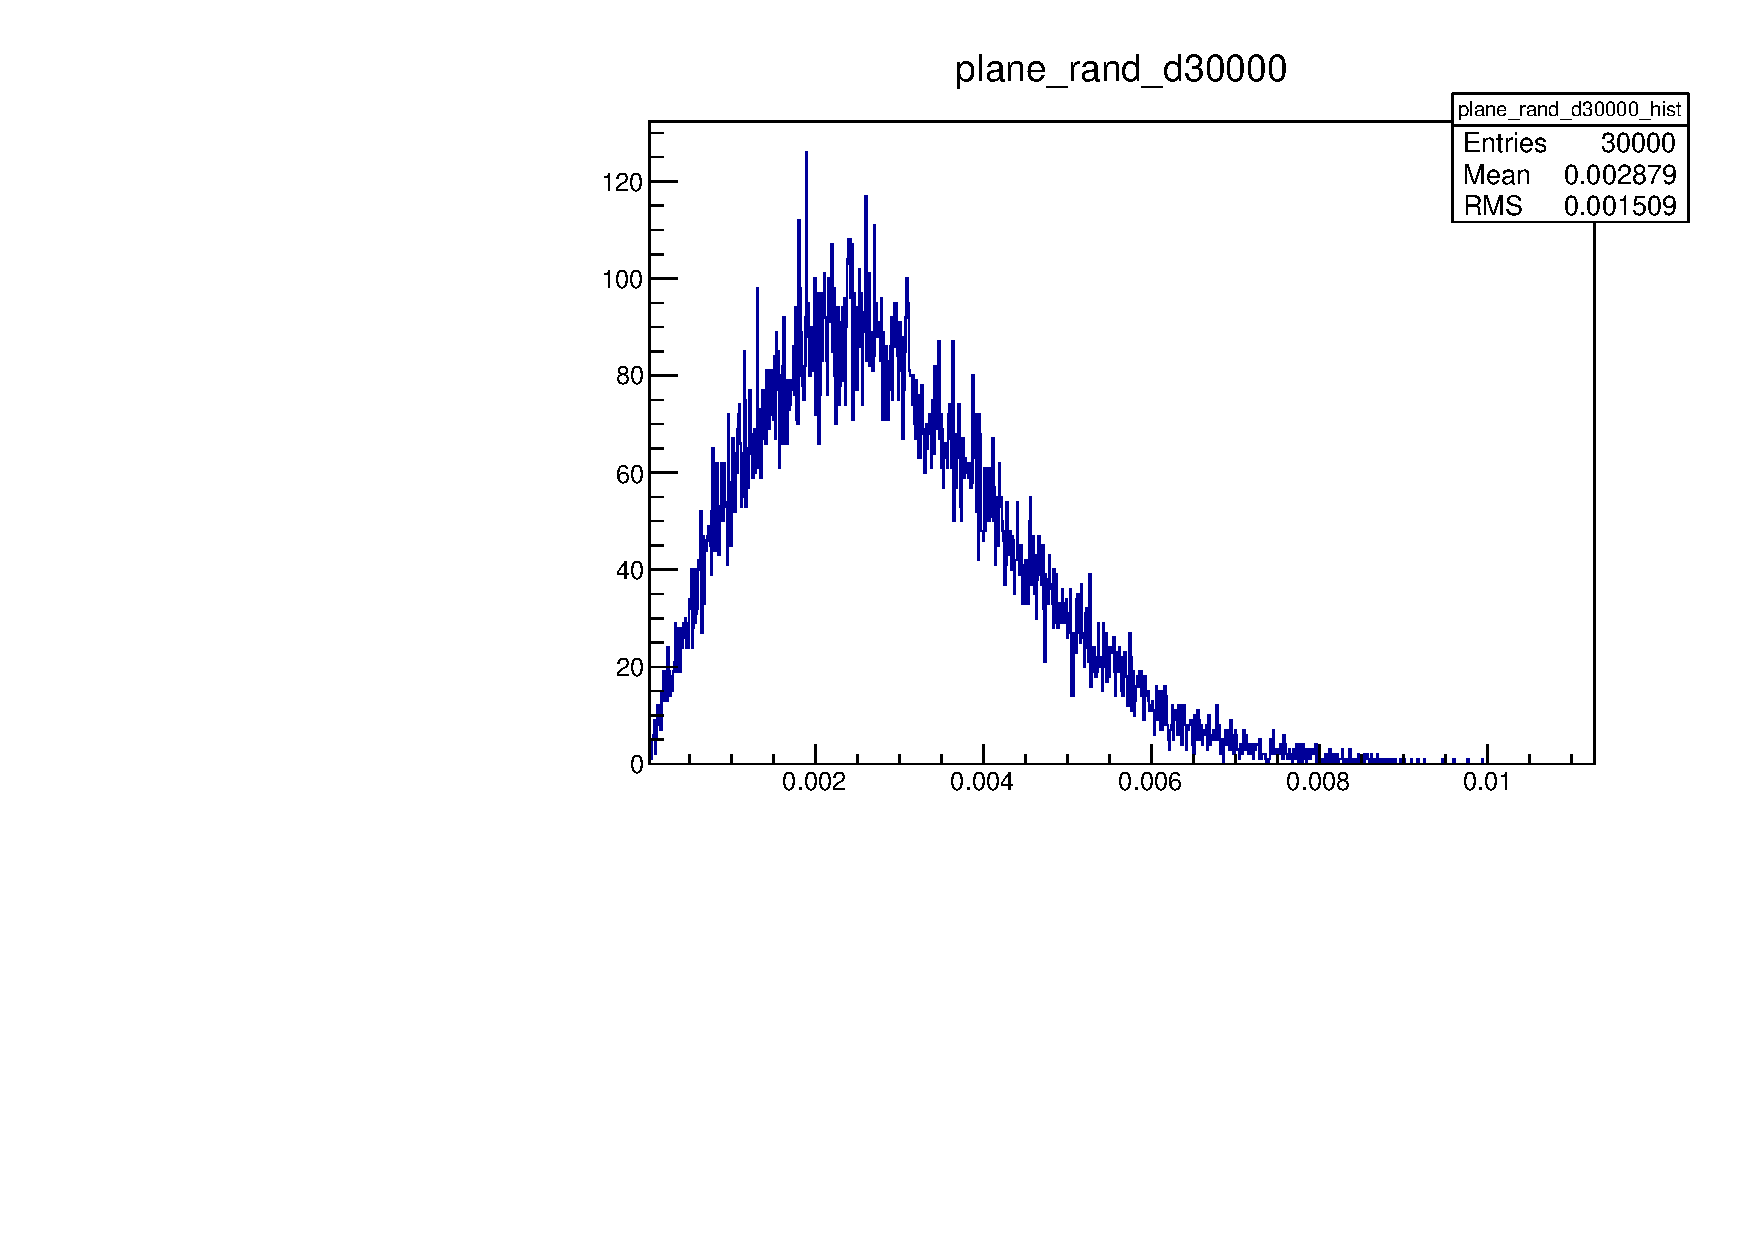
\includegraphics[width=.6\textwidth]{fig/plane_rand_d30000.pdf}
\caption{Same as figure \ref{fig:plane_rand_d30000} but with randomly dispersed samples $q \in Q$}
\label{fig:plane_rand_d30000_randQ}
\end{figure}


When working with artificially generated, perfectly aligned point clouds with a square grid point dispersion, the side lengths $l_P$ and $l_Q$ for the model and the sample point clouds must be chosen such that $\frac{l_P}{l_Q} \notin \mathbb{Q}$, otherwise same placements of sample points relative to model points will repeat, and a larger number of sample points doesn't increase histogram quality. For example if $l_P = 0.1$ and $l_Q = 0.02$, each square of the model will have $25$ sample points placed within it at the same relative positions. Taking into account that floating point numbers with limited precision are used, it means that when considering $l_P$ and $l_Q$ to be rational numbers, they should be chosen such that their least common multiple should is as high as possible.


\subsection{Plane with square grid dispersion}
Figure \ref{fig:plane_cphist} shows the distance histogram of two perfectly aligned planar surfaces $P$ and $Q$, where the points on $P$ are dispersed on a square grid. $\rho(P) = 20000$ and $30000$, respectively. The number of samples is $N(Q) = 300000$.

\begin{figure}[H]
\centering
\begin{subfigure}{.5\textwidth}
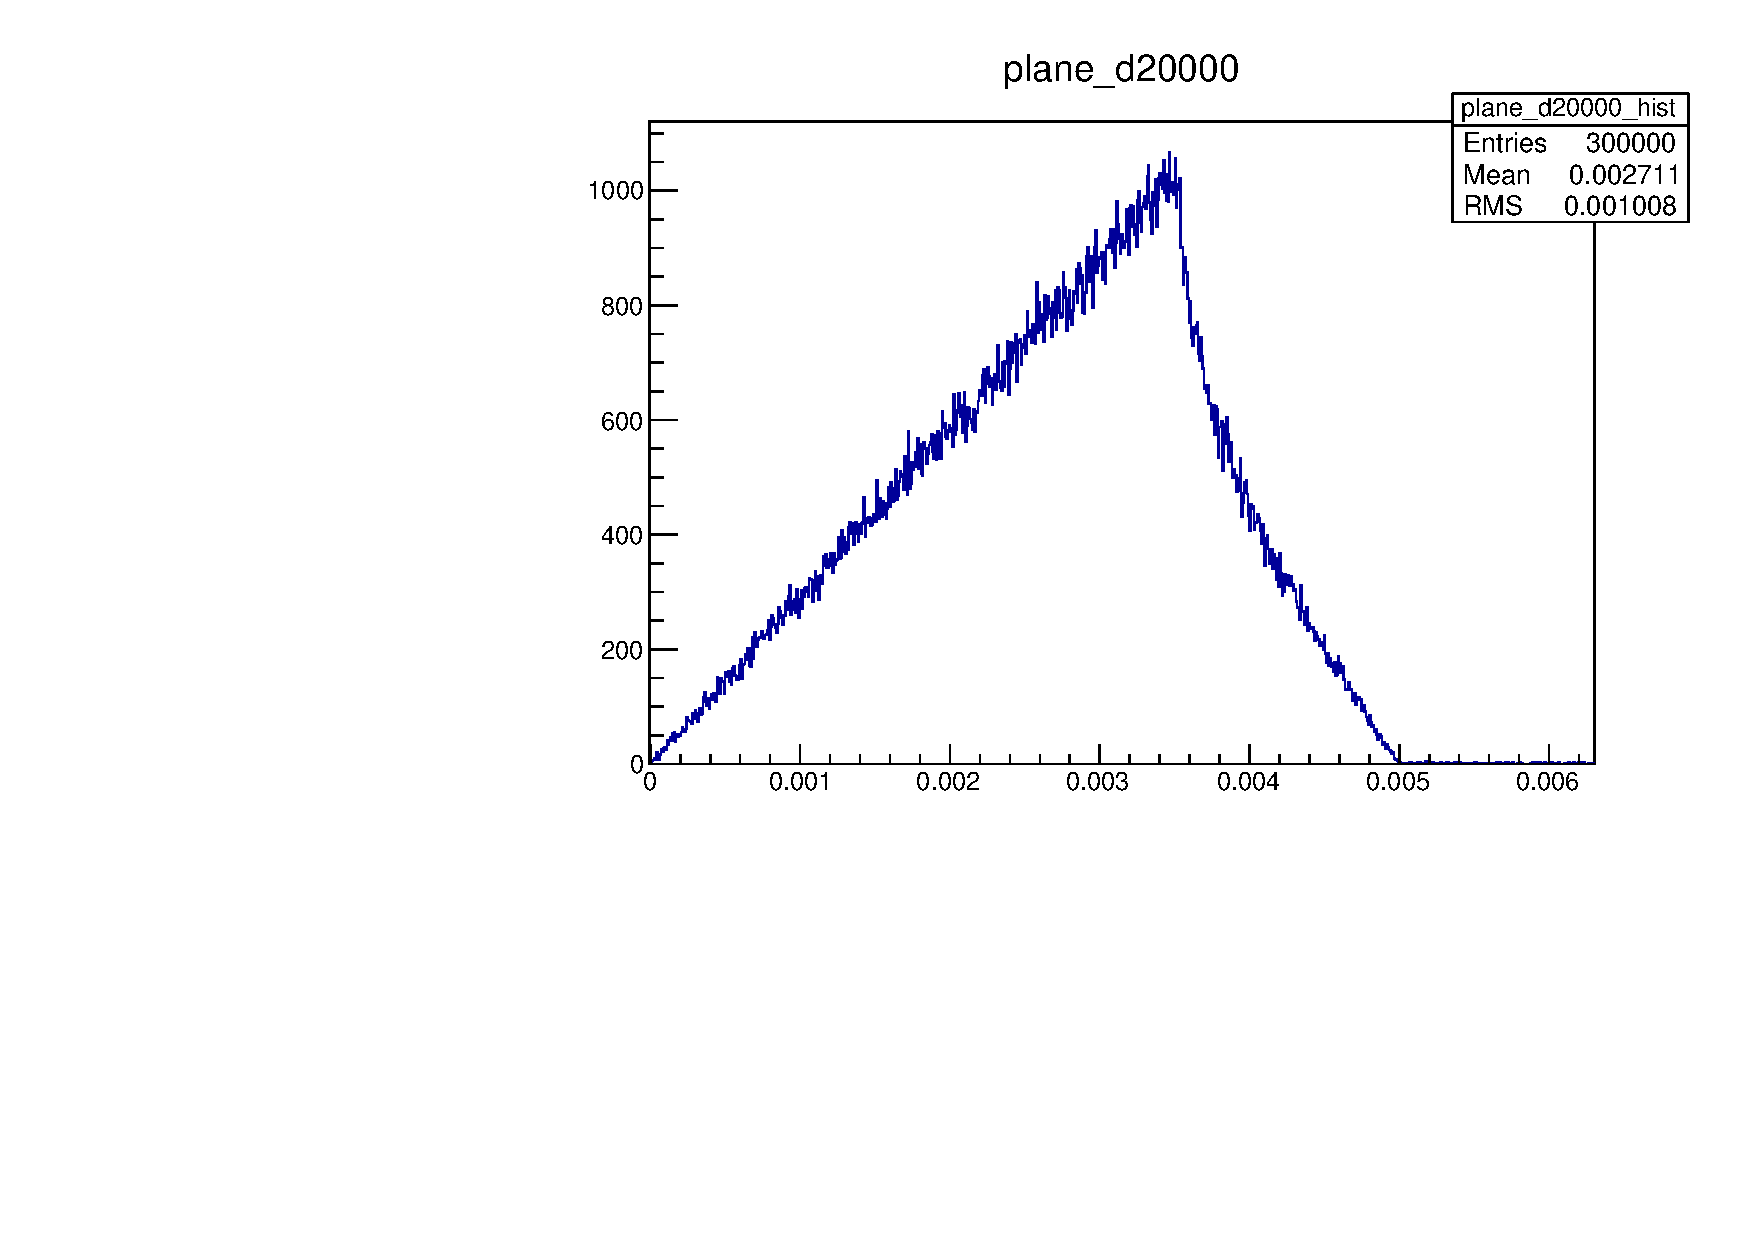
\includegraphics[width=\linewidth]{fig/plane_d20000.pdf}
\end{subfigure}%
\begin{subfigure}{.5\textwidth}
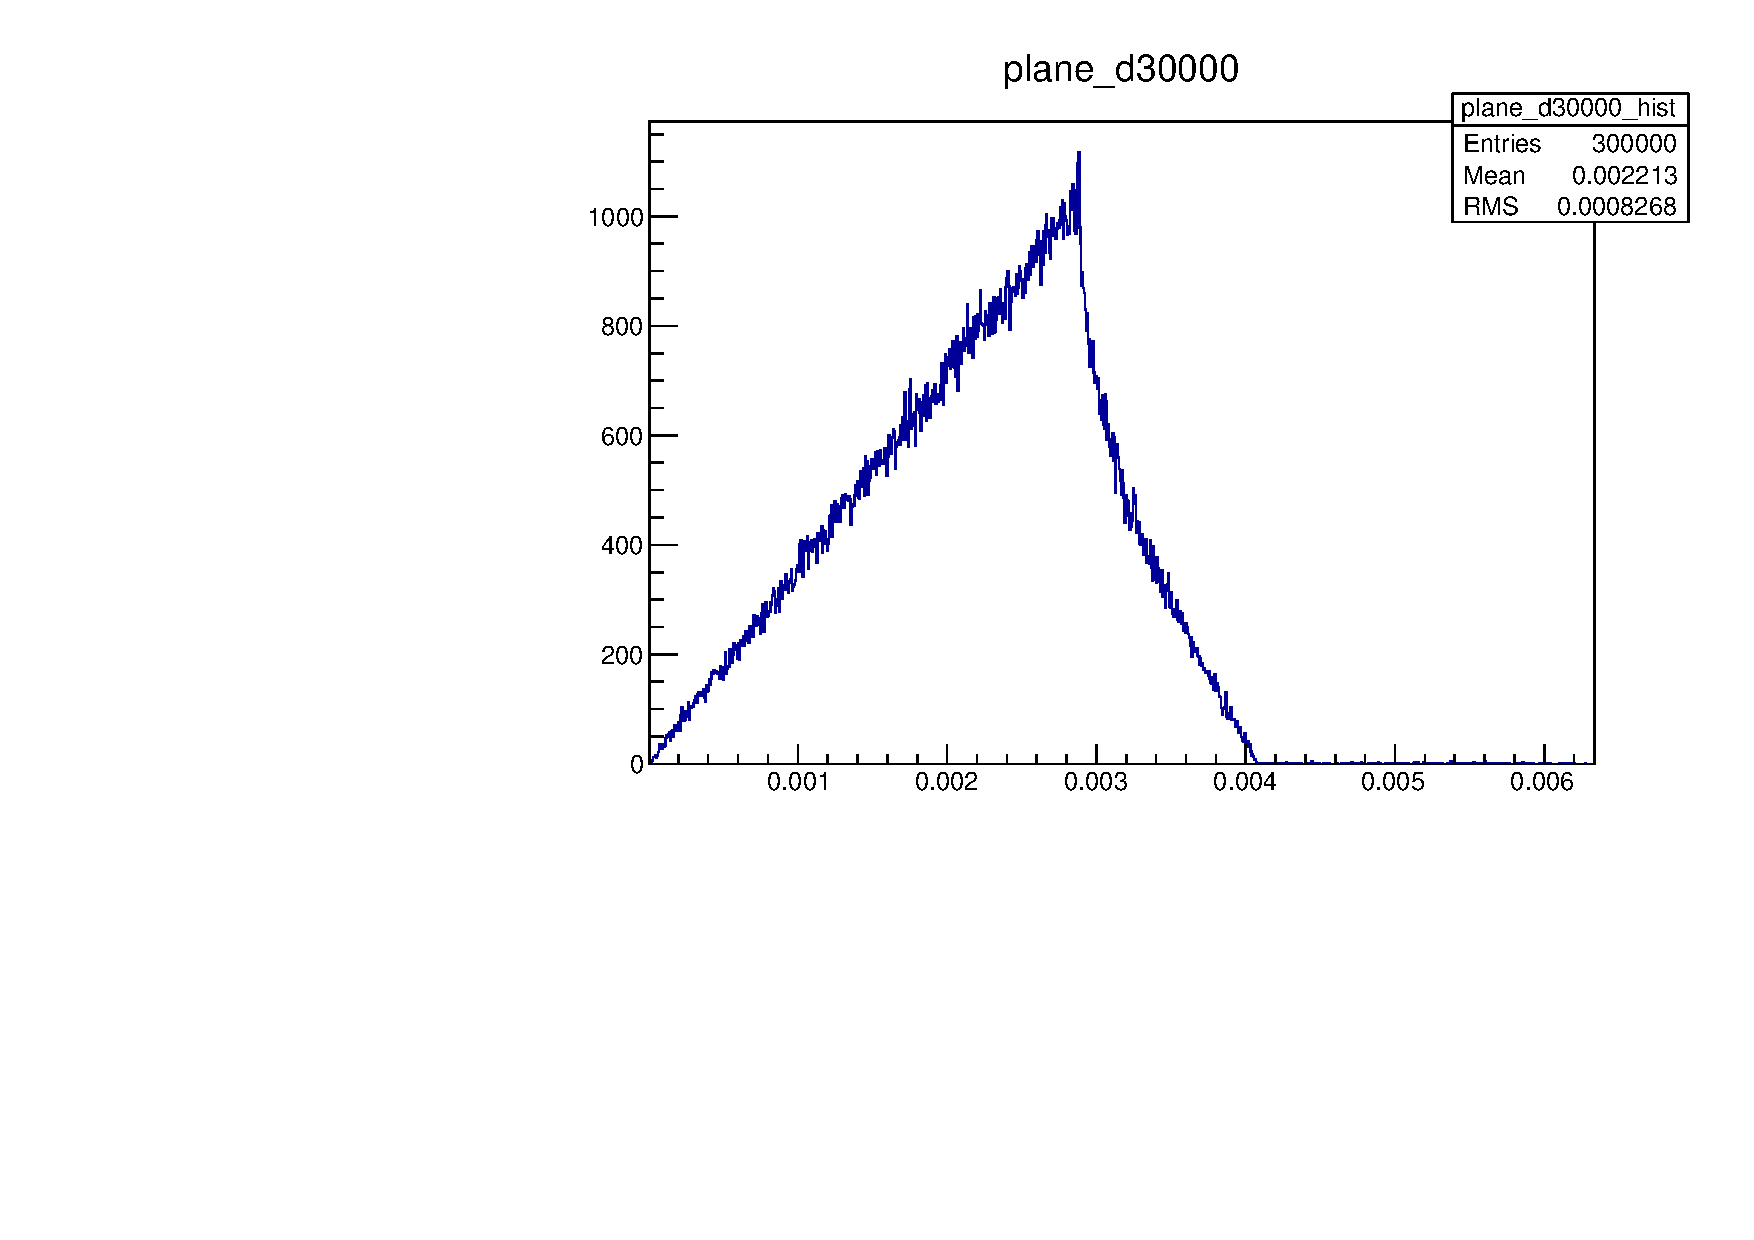
\includegraphics[width=\linewidth]{fig/plane_d30000.pdf}
\end{subfigure}
\caption{Own distance histogram for plane $P$ with square grid point dispersion}
\label{fig:plane_cphist}
\end{figure}

The probability density function $f_R$ is
\begin{equation}
f_R(r) = \frac{r}{2 l} \times \begin{cases}
	\frac{\pi}{4} & 0 \leq r \leq \frac{l}{2} \\
	\frac{\pi}{4} - \arctan{\sqrt{\left( \frac{2r}{l} \right)^2 - 1}} & \frac{l}{2} < r < \frac{l}{2} \sqrt{2}
\end{cases}
\end{equation}
with $l = \frac{1}{\sqrt{\rho(P)}}$. This is proven in appendix \ref{sec:proof_sqgrid_disp_plane}. The plot is shown in figure \ref{fig:sq_grid_d} for $l = 2$.

The probability rises linearily from $O$ to to its mode at $r = \frac{l}{2}$. Within that range, the sample point falls within the non-overlapping disks of radius $\frac{l}{2}$ around the model points.

\begin{figure}[p]
\centering
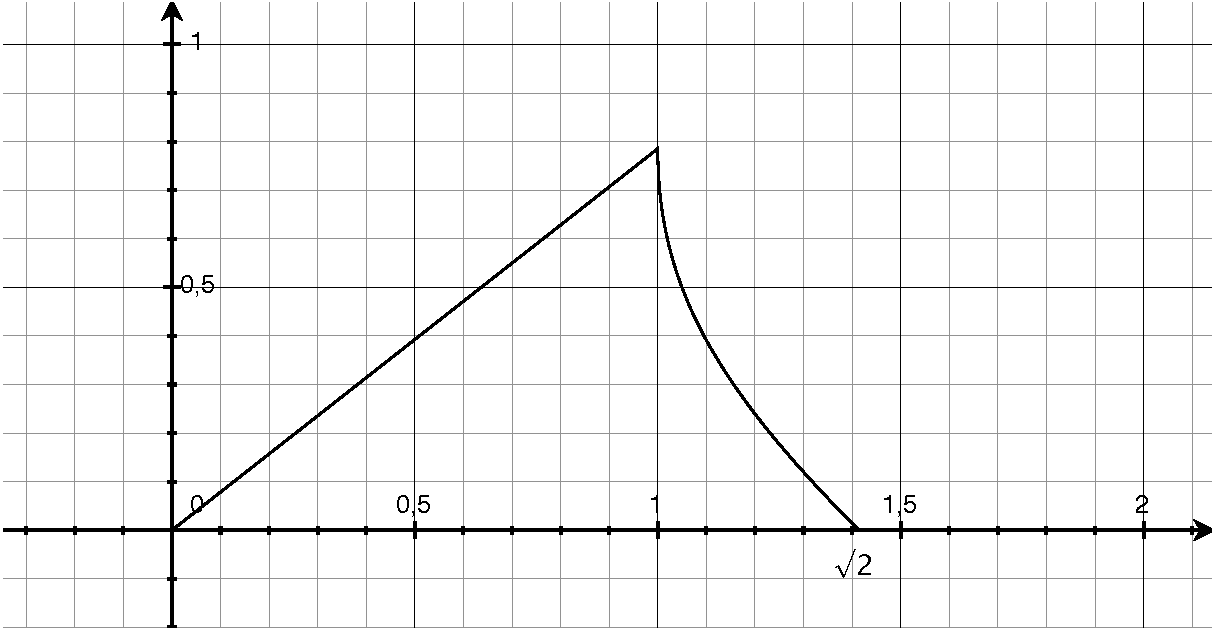
\includegraphics[width=.5\textwidth]{fig/sq_grid_d.pdf}
\caption{Probability density function of closest point distance, for plane $P$ with square grid point arrangement}
\label{fig:sq_grid_d}
\end{figure}


\subsection{Plane with parallelogram grid dispersion}
The square grid dispersion in a special case of the parallelogram grid dispersion. Figure \ref{fig:plane_par_cphist} shows an example of an own closest point histogram obtained when the model point cloud has a parallelogram grid point dispersion. As seen on figure \ref{fig:pargrid_proj}, it is the result of a parallel projection of a square grid on the camera image frame onto a plane in space with a normal vector $\vec{n}$, relative to the camera's coordinate system. For this example, $\vec{n} \approx \transpose{(-0.253023, 0.787174, -0.562438)}$, and the square grid on the image plane has a side length of $p_l = 0.067$.
s
Figure \ref{fig:par_grid} is a close-up view of the plane, showing the parallelogram grid of $P$, and the higher density square grid sample point cloud $Q$ in blue.


\begin{figure}[H]
\centering
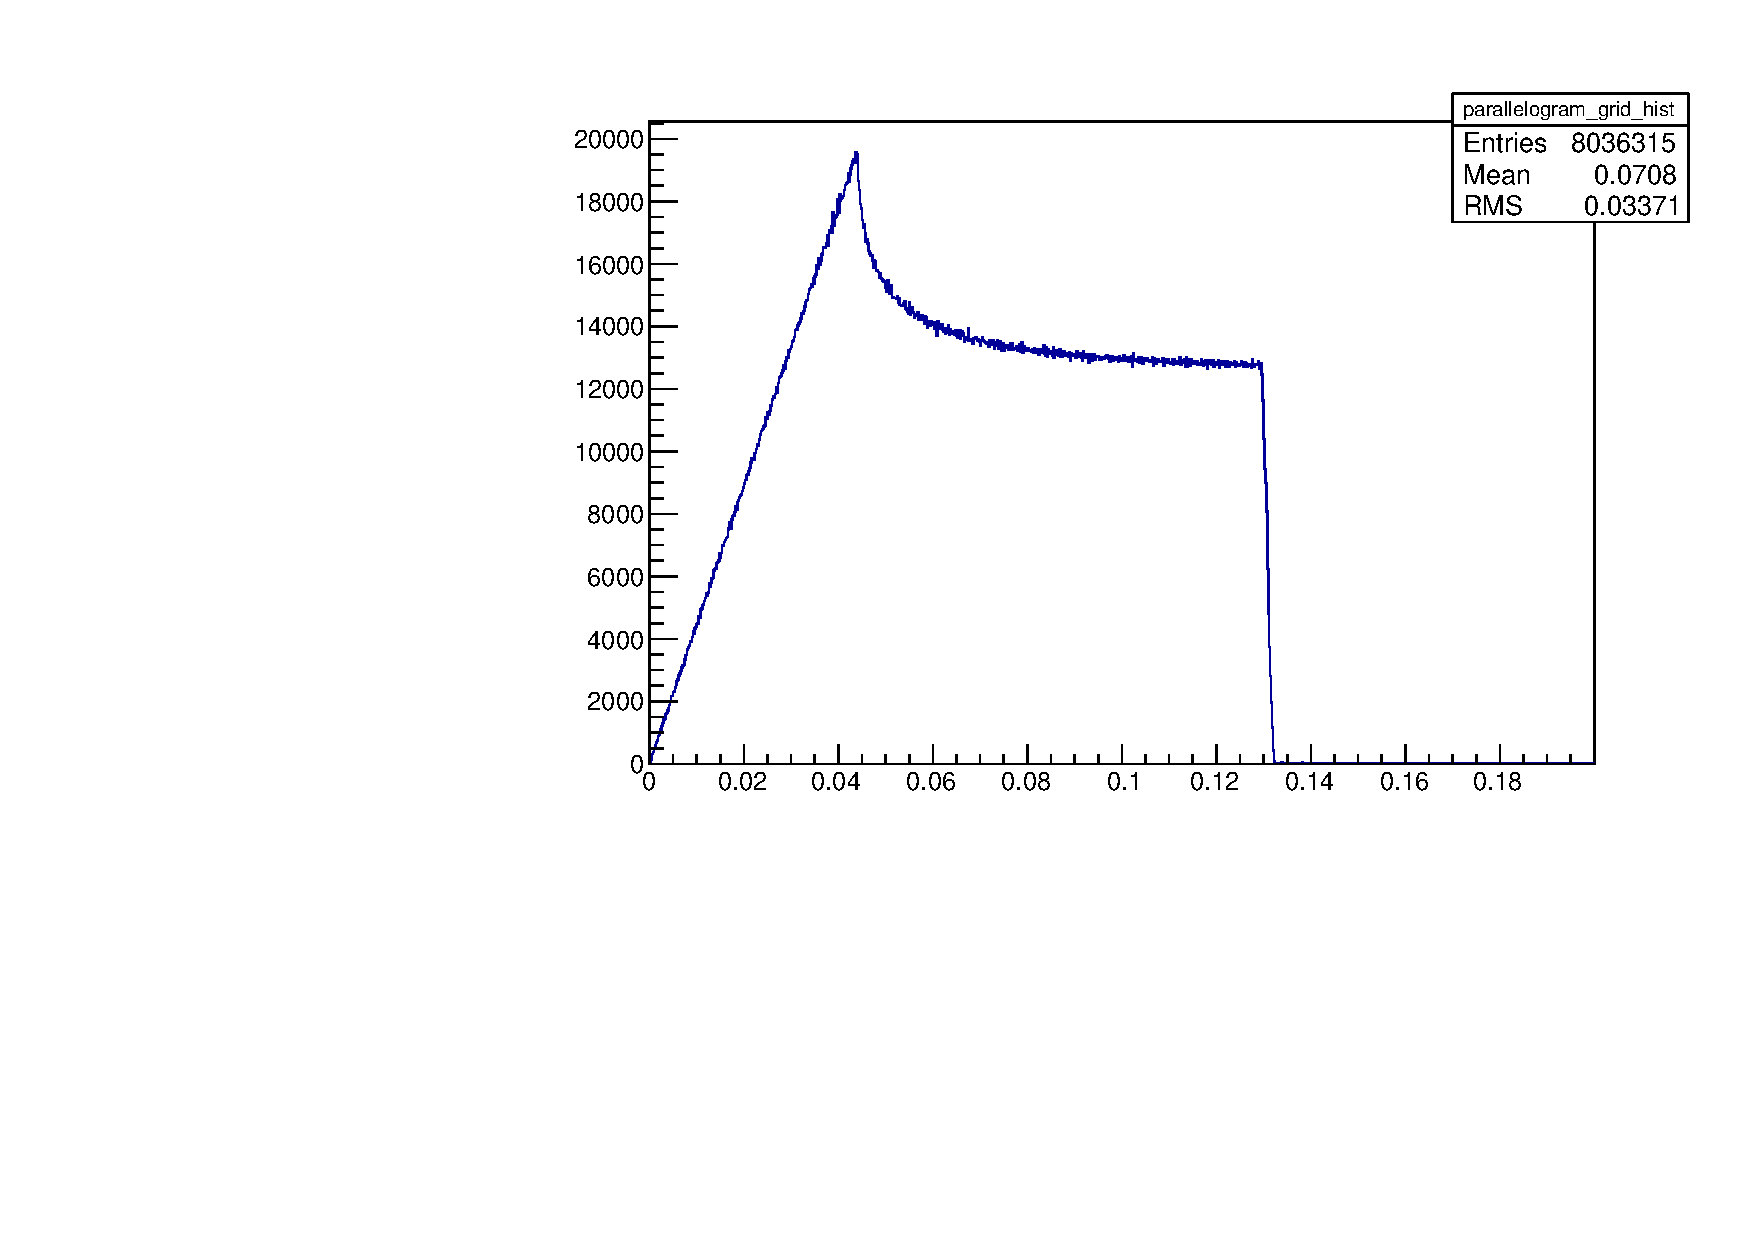
\includegraphics[width=.5\textwidth]{fig/parallelogram_grid.pdf}
\caption{\gls{Gls} for plane $P$ with parallelogram grid point dispersion}
\label{fig:plane_par_cphist}
\end{figure}

It can be seen that the histogram's underlying probability density function is again a piecewise function, and that its first segment is still a linear increase from the zero point to the mode of the histogram.

Using a similar argument as for the square grid dispersion, one can show that the linear increase happens from $0$ to $\frac{1}{2} l_\text{min}$. Applying the formula \ref{eq:pargrid_lmin} developed in the previous section, a value of approximatively $0.0441$ is found for this example. It corresponds to the mode seen on the histogram.

This segment of linear increase will be called the \acrfull{roi} of the histogram. It will be used to construct an error metric.

\begin{figure}[p]
\centering
{
	\setlength{\fboxsep}{0pt}%
	\setlength{\fboxrule}{0.5pt}%
	\fbox{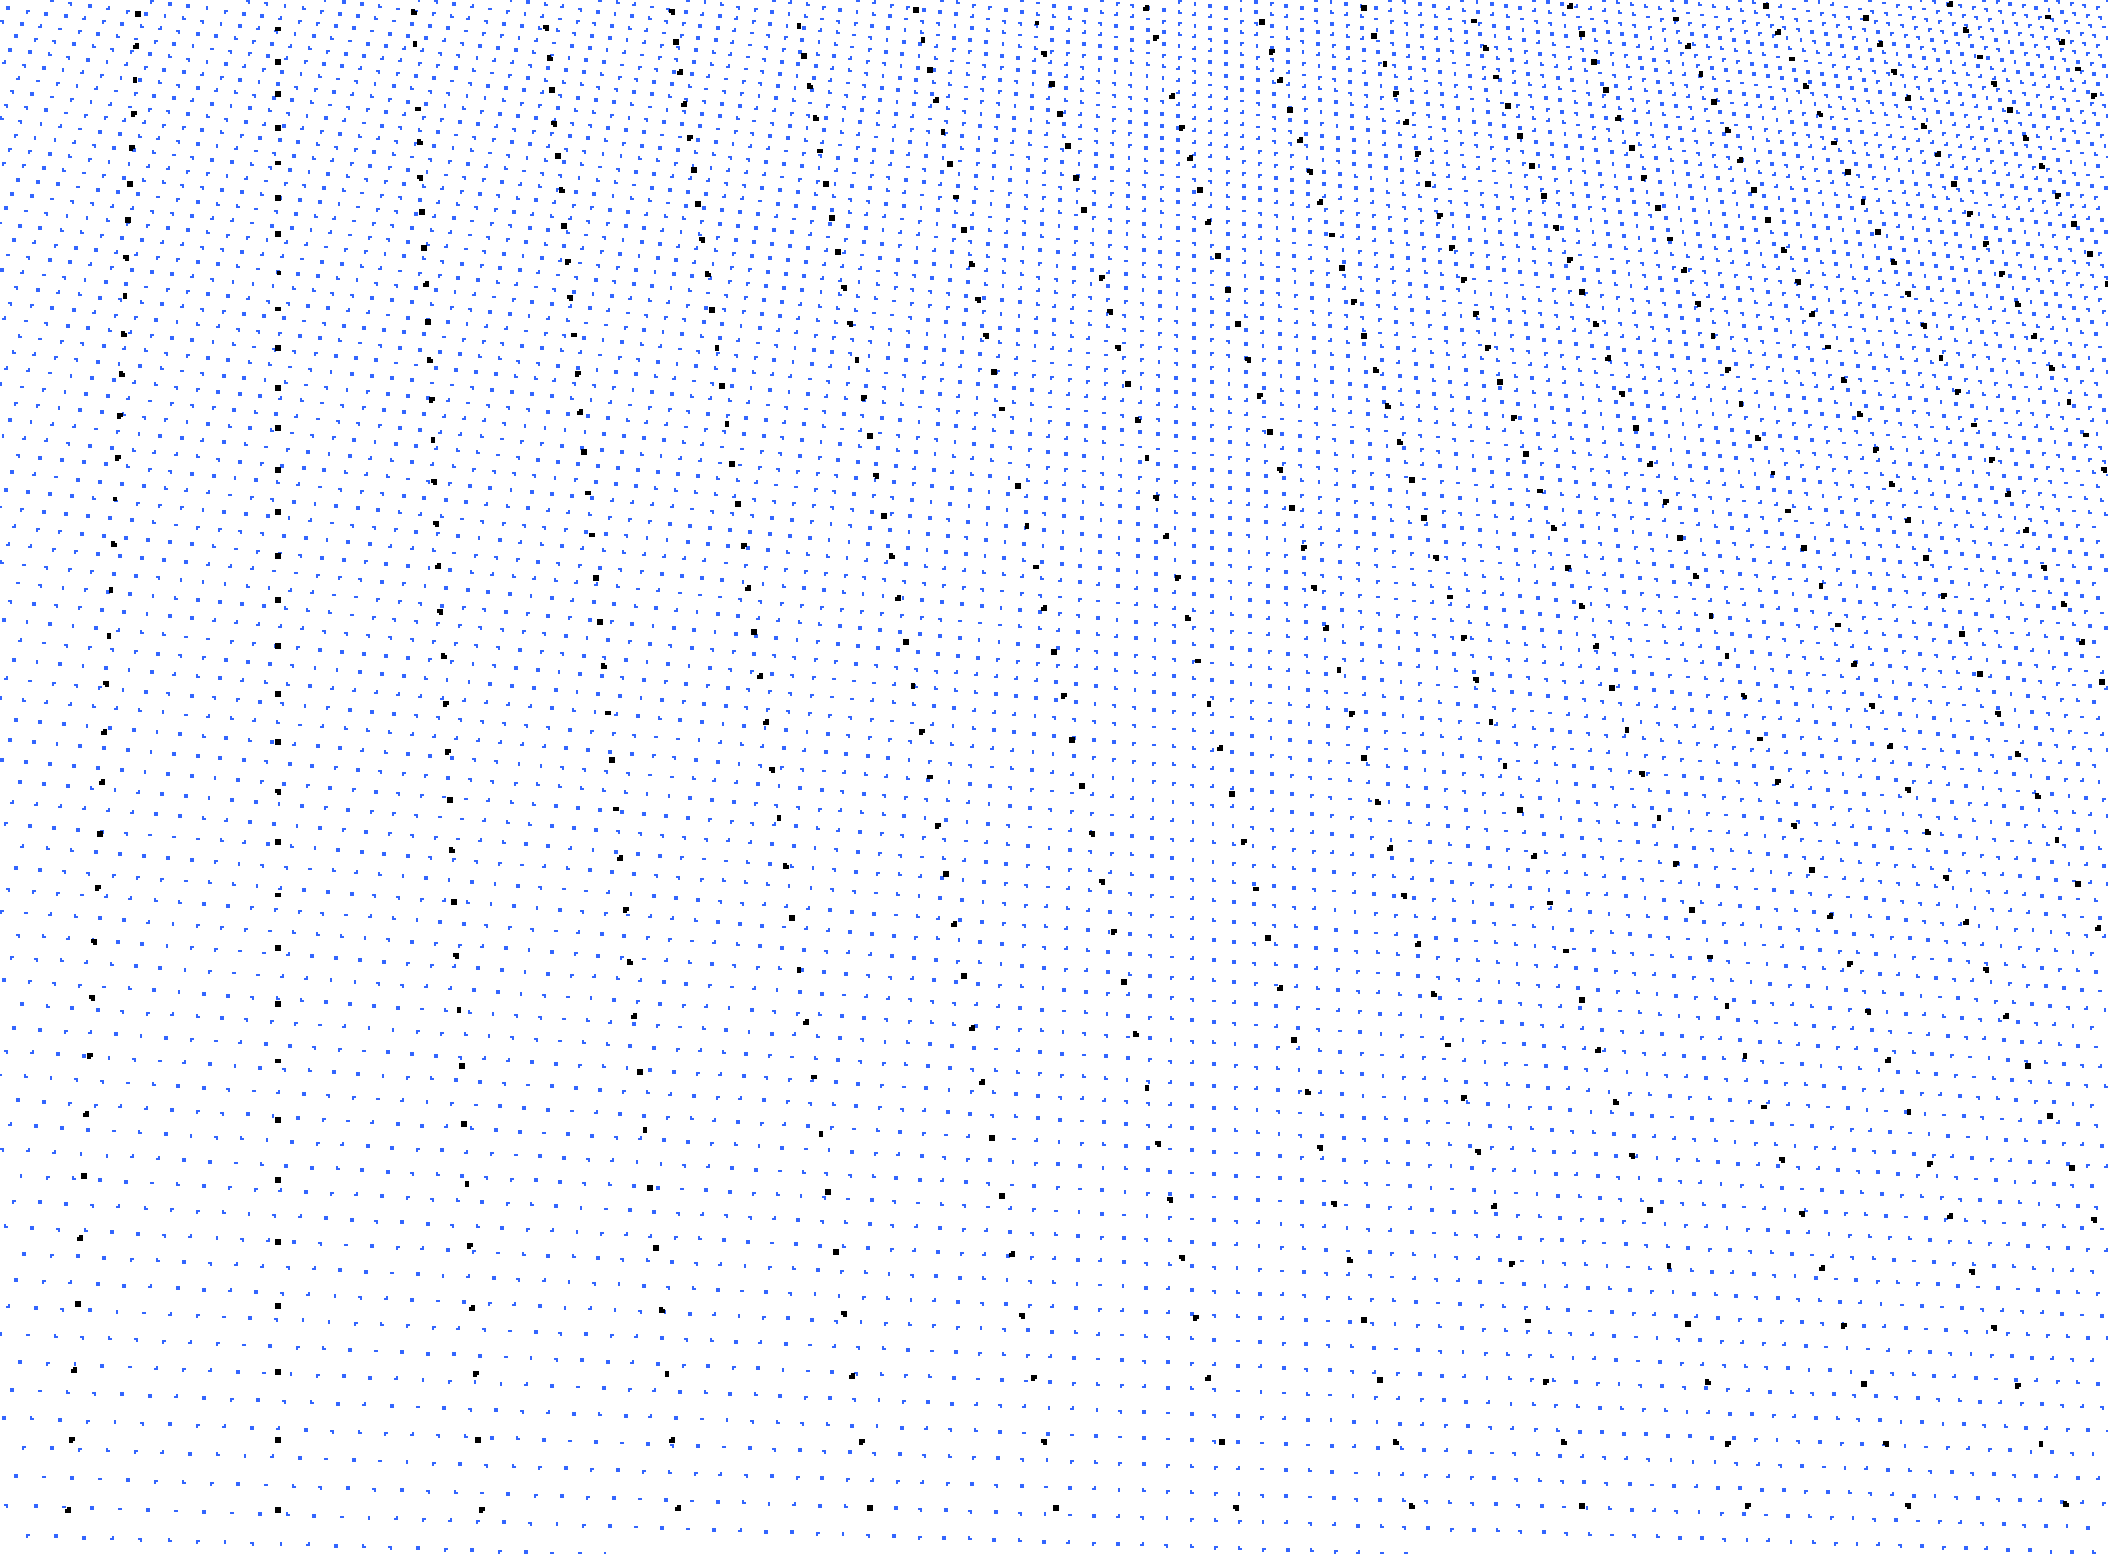
\includegraphics[width=.5\textwidth]{fig/closeup_pargrid.png}}%
}
\caption{Close-up view of parallelogram grid in $P$ (black), and sample point cloud $Q$ (blue)}
\label{fig:par_grid}
\end{figure}



\subsection{Adjusted own distance histogram}
It is possible to calculate the range of the \gls{roi} of the histogram, using only the plane's normal vector $\vec{n}$ and the side length $p_l$ of the parallel projection camera. Here an attempt is made to use this result to produce an \acrfull{aodh}, which still has the initial linear increase, for point clouds that are not planes.

When the surface is no longer a plane, $\vec{n}$ will no longer be constant, but can have a different value for each point. However for smooth surfaces on the model, the normal vector will remain approximatively constant on local regions of neighboring points, as can be seen on the close-up views in the previous sections. On these planar regions the parallelogram grid point dispersion appears.

Under the assumption that most of the point clouds consists of such planar regions, its own distance histogram will be a superposition of the kinds of parallelogram grid histograms seen before, with an initial linear increasing segment.

\subsubsection{Multi-planes point cloud}
In order to test the shape of this superposition histogram, an artificially generated ``multi-planes'' point cloud is used. It consists of multiple planes places randomly in space at different orientations, projected using a parallel projection camera. An example with two planes is shown in figure \ref{fig:disks1}, shown with decreased point density.

The two planes are bounded to the shapes of disks. This does not have an effect of the histograms, and just makes the point cloud easier to visualize. If the bound was a square, it would change depending on the rotation of the plane on its own axis.

Both planes have the parallelogram grid point dispersion. The example is chosen so that one plane is approximatively facing the camera while the other is more oblique, and has a lower $\rho$ and higher $l_\text{min}$ as a result. Figure \ref{fig:multiplane_cphist} shows the own distance histograms for the two individual planes, and the superposition histogram for the entire multi-planes point cloud.

\begin{figure}[H]
\centering
\begin{subfigure}{.32\textwidth}
	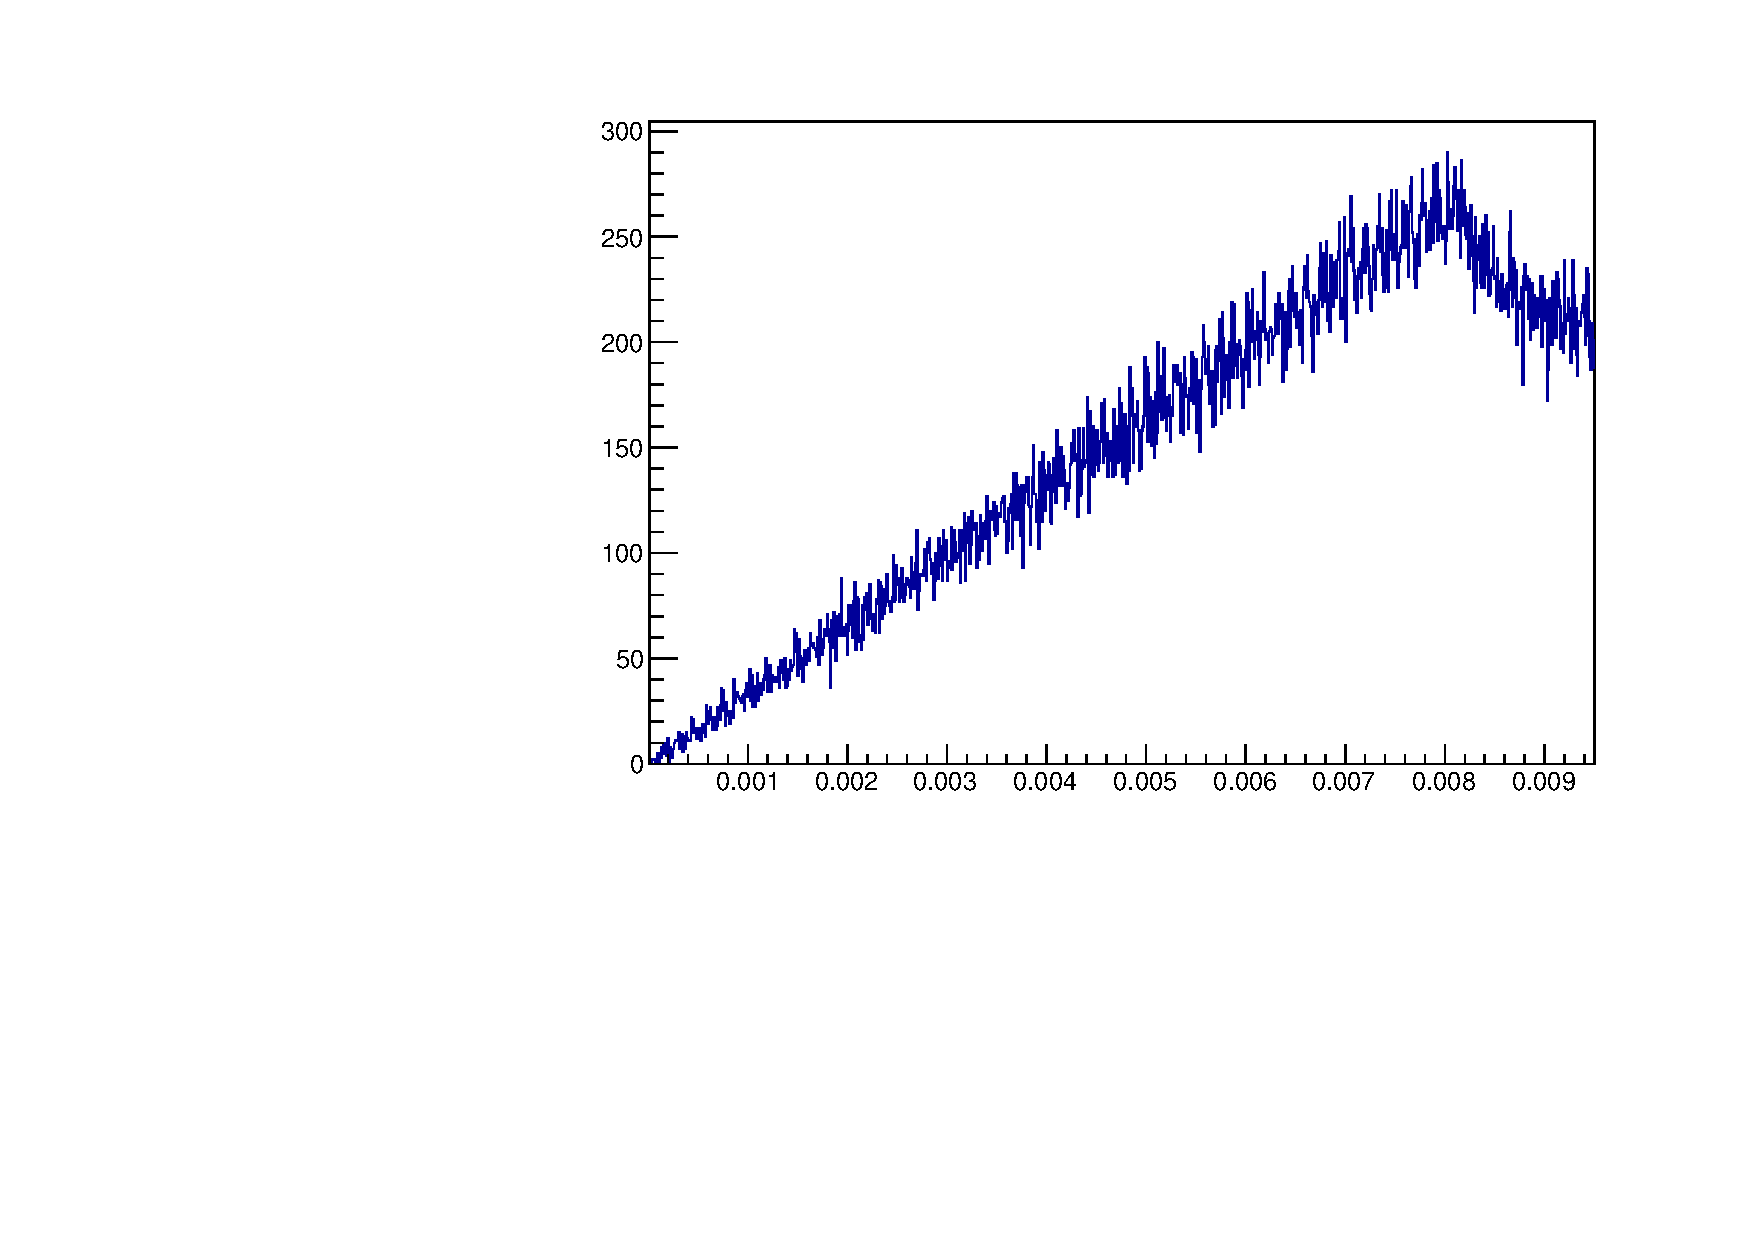
\includegraphics[width=\linewidth]{fig/orig_plane1.pdf}
	\caption{Oblique plane}
\end{subfigure}%
\begin{subfigure}{.32\textwidth}
	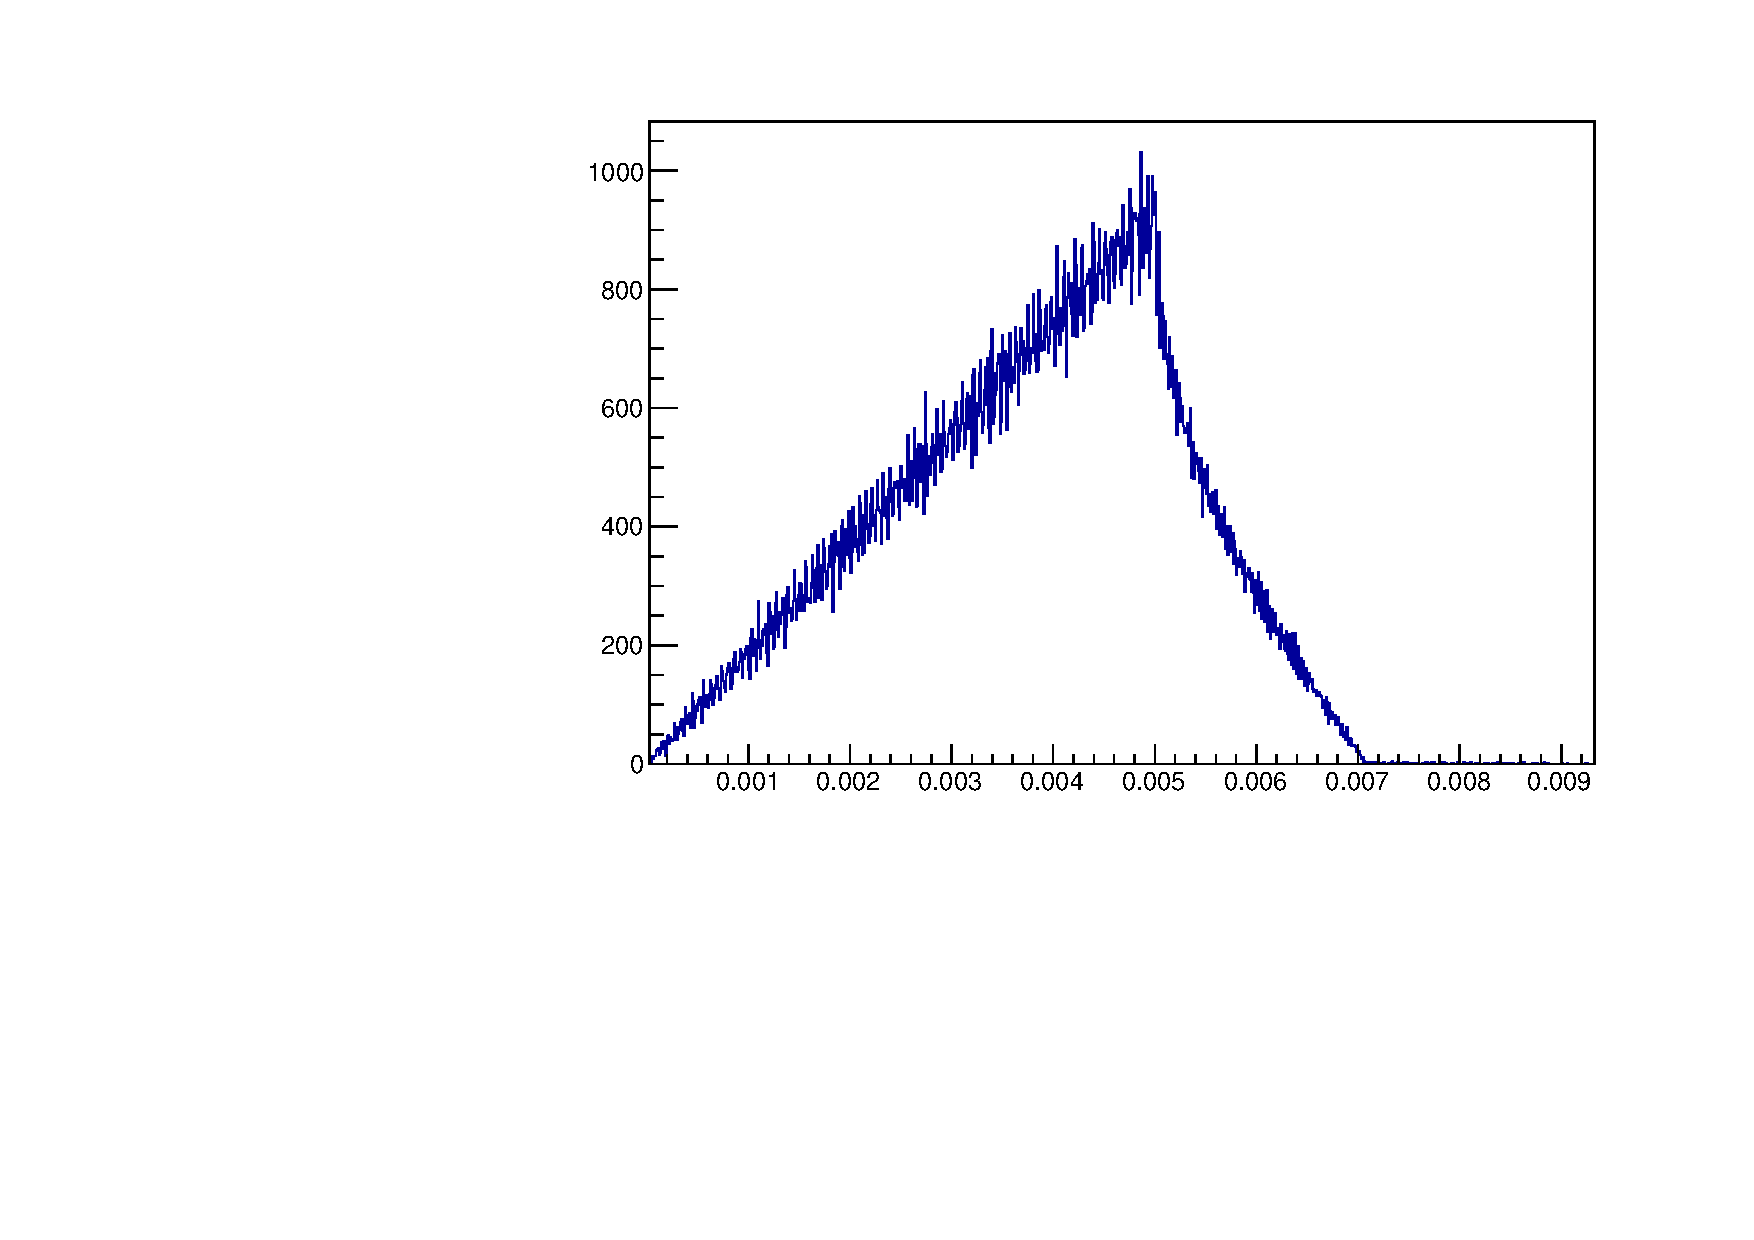
\includegraphics[width=\linewidth]{fig/orig_plane2.pdf}
	\caption{Parallel plane}
\end{subfigure}%
\begin{subfigure}{.32\textwidth}
	\includegraphics[width=\linewidth]{fig/orig_superposition.pdf}
	\caption{Superposition}
\end{subfigure}
\caption{Own distance histogram for multi-plane point cloud $P$ (individual planes, and superposition)}
\label{fig:multiplane_cphist}
\end{figure}

It can be seen that the linear \gls{roi} of the superposition histogram ranges up to about $0.005$, which is the minimum of the ranges on the two individual histograms. Thus the information from the remaining linear range of the oblique plane is lost.

\begin{figure}[p]
\centering
{
	\setlength{\fboxsep}{0pt}%
	\setlength{\fboxrule}{0.5pt}%
	\fbox{\includegraphics[width=.5\textwidth]{fig/disks1.png}}%
}
\caption{Example of multi-plane point cloud}
\label{fig:disks1}
\end{figure}

\subsubsection{Adjusted histogram}
The \gls{aodh} is created as follows: For each $q \in Q$, the closest point $p \in P$ is taken, for which $d = \|p - q\|$ is minimal. Then instead of $d$, the value $d' = \frac{2 \, d}{l_{\text{min}}(\vec{n})}$ is recorded in the histogram. $l_{\text{min}}$ is calculated from the normal vector $\vec{n}$ of $p$ using the approximation formula \ref{eq:pargrid_lmin}. Samples are only added to the histogram when the threshold condition \ref{eq:pargrid_lmin_cond} is met.

All the histograms created from subsets of the point cloud containing only regions of the surface with an approximatively constant normal vector $\vec{n}$, would have a linear increase until $d = \frac{1}{2} \, l_{\text{min}}(\vec{n})$. The adjusted own distance histogram is a superposition of these, distorted such that its \gls{roi} ranges from $d' = 0$ to $d' = 1$.

The following figure \ref{fig:disks_adj} shows this \ghs{aodh}, in comparison to the non-adjusted \gls{odh}, for the same point cloud $P$. $P$ is a multi-planes as before, but with more planes. Figure \ref{fig:relief_adj} shows the same histograms where $P$ and $Q$ is a relief point cloud. It appears more irregular than the \gls{odh}, but the \gls{roi} contains a higher number of samples.
\begin{figure}[H]
\begin{subfigure}{.5\textwidth}
	\includegraphics[width=\linewidth]{fig/disks_noadj.pdf}
	\caption{Non-adjusted histogram}
\end{subfigure}%
\begin{subfigure}{.5\textwidth}
	\includegraphics[width=\linewidth]{fig/disks_adj.pdf}
	\caption{Adjusted histogram}
\end{subfigure}
\caption{\Gls{odh}, and \gls{aodh} of $P$}
\label{fig:disks_adj}
\end{figure}


\begin{figure}[p]
\begin{subfigure}{.5\textwidth}
	\includegraphics[width=\linewidth]{fig/relief_noadj.pdf}
	\caption{Non-adjusted histogram}
\end{subfigure}%
\begin{subfigure}{.5\textwidth}
	\includegraphics[width=\linewidth]{fig/relief_adj.pdf}
	\caption{Adjusted histogram}
\end{subfigure}
\caption{\Gls{odh}, and \gls{aodh} of relief point cloud}
\label{fig:relief_adj}
\end{figure}



\subsection{Occlusion and different bounds}
Point clouds obtained from real scans will not cover the entire surface due to occlusion, and any two point clouds $P$ and $Q$ will have different bounds. Thus there can be sample points $q$ on surface positions that are not covered by $P$, and vice versa.

It is assumed that ideally the parallelogram grid on $P$ is the same everywhere, and that the point dispersion on locally planar surface parts depends only on the local normal vector. Therefore when part of the sample point cloud $Q$ are removed, it only decreases the quality of the histogram as there are less samples, but does not alter its shape.

However when parts of the model point cloud $P$ are removed, for sample point $q \in Q$ that fall within these regions, the closest point $p \in P$ will be much farther away. As a result much greater distances are recorded, than for the samples falling within the parallelogram grid of $P$.

These distance values add more samples on the right side of the histogram, and do not affect the shape of the \gls{roi} of the histogram.

In the histograms on figure \ref{fig:relief_adj}, $P$ is a sideways view-point of the relief model, and it can be seen that the \gls{odh} contains samples at greater distances, at a low but near constant rate. When zoomed out, this extends to a much longer range.


\subsection{Sample for real point cloud}
When $P$ is not an artificially generated point cloud but is taken from a 3D scan, the sample $Q$ cannot easily be constructed as the surfaces are unknown.

Using the scan as sample and a dowmsampled version of it as model does is not possible, because downsampling removes the properties of the point dispersion. The histogram of the nearest neighbor distances, that is, the distance from each point in $P$ to the closest point in $P$ except for itself, does not produce an \gls{odh}.

One approach to construct a higher resolution sample $Q$ from the point scan $P$ is the following:
\begin{enumerate}
\item $P$ is supposed to be a range image. Its camera position is at the origin of its coordinate system. As shown in section \ref{sec:estimate_proj_par}, $p_l$ and $l_{\text{min}}$ are be estimated from the point cloud.
\item All points from $P$ which no not satisfy the threshold condition for obliqueness \ref{eq:pargrid_lmin_cond}, and the points for which the local surface curvature is too large, are removed.
\item $Q$ is initialized to an empty point cloud.
\item For the \gls{aodh}, points with $d > \frac{1}{2} l_{\text{min}}$ will fall outside its \gls{roi}, so $Q$ does not need to include those.

A copy $P'$ of $P$ is constructed, and each of its points $p$ is randomly displaced along its tangent plane. The tangent plane is calculated using each point's normal vector. The random displacement along the polar coordinates $r$ and $\theta$ on this plane, centered on the point $p$, is done according to an uniform distribution with  $r \in [0, \frac{k}{2} l_{\text{min}} ]$ and $\theta \in [0, 2 \pi]$, where $k \geq 1$ (and not smaller than $1$). It can be set to a greater value to compensate for when the scanner rays are actually not parallel.
\item $P'$ is fused into $Q$. Then step $4$ is repeated, for a total of $N$ times.
\end{enumerate}
The resulting sample point cloud $Q$ now has $N$ times the number of points than $P$, its still lie on the object surfaces (assuming $P$ is locally planar in the direct neighborhood of its points), and they are uniformly distributed around the points.

\subsubsection{Results}
The \gls{aodh} obtained from the \gls{ddp} point cloud as $P$, and a sample point cloud $Q$ constructed from it with this method, is shown in \ref{fig:ddp_adj}. It still shows the linear increase in the \gls{roi}. However this result is not surprising, since $Q$ was specifically constructed to have an uniform distribution of the displacement radii $r$ on the tangent planes.

The idea is that if another, higher resolution scan of the same object is used as $Q$, the linear increase should also be present, but only when the point clouds are perfectly aligned. Measuring how linear the \gls{roi} is should give an indication of how well $P$ and $Q$ are aligned.

\begin{figure}[h]
\centering
\includegraphics[width=.5\textwidth]{fig/ddp_adj.pdf}
\caption{\Gls{aodh} for \gls{ddp} $P$ from constructed sample point cloud $P$}
\label{fig:ddp_adj}
\end{figure}

\FloatBarrier

\newpage

\section{Cross distance histogram}
Up until now $P$ and $Q$ were considered to represent the same surface and be perfectly aligned. For the \gls{cdh} this last constraint is removed, so there is a rigid transformation $\matr{M}$ which aligns $P$ to $Q$.


\subsection{Adjusted histogram}
As before the \gls{acdh} is constructed from the distances of the sample points $q \in Q$ to their closest point $p \in P$.

To reduce the number of wrong correspondences, they are only accepted when the normal vectors of $p$ and of $q$ are \emph{compatible}, that is, the angle $\arccos \vec{n}(p) \, \vec{n}(q)$ is below a fixed threshold value. If the normals point in different directions, the points do not represent the same locations on the surface. Also, correspondences where $d(p, q)$ is above a fixed maximal distance are rejected.

Because the surfaces are no longer perfectly aligned, the distribution of the distances $d = d(p, q)$ will be different. Whenever $q$ is at a distance from the surface of $P$ on which $p$ lies, $q$ no longer falls into the two-dimensional parallelogram grid, and $d$ will be larger. Hence the more $\matr{M}$ deviates from $\matr{I}$, the more the distribution of $d$ will deviate from the one from the \gls{aodh}, and it will no longer have the characteristic linear increase from $d = 0$ to $1$.


\subsection{Rejection histogram}
In addition to this \gls{acdh} the \acrfull{arcdh} will be considered. Here the sample points $q \in Q$ are projected onto the surface of $P$, and then the distance from this \emph{projected point} $q_{{proj}}$ to $p$ is measured and recorded into the histogram. The projected point is calculated using the normal vector of $p$, denoted $\vec{n}_p$:
\begin{equation}
\vec{q}_{\text{proj}} = \vec{q} - \left[ \vec{n}_p (\vec{q} - \vec{p}) \right] \vec{n}_p
\end{equation}
And the distance $d_{\text{proj}} = \| \vec{q}_{{proj}} - \vec{p} \|$ is recorded. The vector $\vec{q}_{{proj}} - \vec{p}$ is also called the \emph{rejection}.

$p$ is still computed as the closest point to $q$ and not to $q_{\text{proj}}$, as otherwise the closest point algorithm would have to be run twice. This should not have a noticeable impact on the results.

Assuming that $\vec{n}_p$ is accurate, $\vec{q}_{\text{proj}}$ is placed on the surface, and as a result the histogram should take on the shape of the \gls{aodh}. However the sample points $vec{q}_{\text{proj}}$ are no longer as evenly distributed. When $Q$ is rotated relative to $P$, they will tend to cluster together more in areas further from the center of rotation. As shown before in \ref{sec:disp_sample_pts}, more variance in the density of the sample points leads to a more jagged histogram.

Also, unlike the \gls{acdh}, this \gls{arcdh} is, ideally, based solely on the dispersion patterns of the points of the surface, and does not take the distances of the surfaces of $P$ and $Q$ into account.


\subsection{Measure of alignment}
In order to find out how the \gls{acdh} and \gls{arcdh} change when a small rigid transformation is applied to $P$, several small translations and rotations were tested. The model is same artificial relief model as in the end of the previous section. For $P$ it is projected from a sideways angle. Results are shown and commented in appendix \ref{sec:relief_small_trans_exp}.

The goal was to construct a numerical error metric which indicates how well $\matr{M}$ aligns $P$ and $Q$. For this the adjusted cross distance histogram is compared to the hypothetical linear increase from $d = 0$ to $1$, using one of the measures described in section \ref{sec:histogram_comp}.

Figure \ref{fig:hist_tri} shows a observed histogram, along with the expected linear increase. The samples with $d > 1$ are discarded. The bins of the histogram are set to have equal width $w$. On the figure $w$ is exaggerated, and neither the observed values nor the expected values (i.e. the blue line) are drawn with the correct bin size.

\begin{figure}[h]
\centering
\includegraphics[width=.5\textwidth]{fig/hist_tri.png}
\caption{Representation of observed and expected histogram}
\label{fig:hist_tri}
\end{figure}

The ``height'' $h$ of the histogram at $d = 1$ is unknown, and depends on the bin width. Because the range is $1$, the area under the histogram curve is equal to the total number of included samples $n$. If the shape is precisely the linear increase, it should be equal to the area of the triangle formed by the blue lines, which is $A = \frac{1}{2} \times 1 \times h = \frac{h}{2}$. So $h = 2 \times n$.

The number $o_i$ of observed values which fall into one bin of width $w$, centered at $d_i$, is the number of samples $d$ such that $d_i - \frac{w}{2} < d < d_i + \frac{w}{2}$. The corresponding expected value is then calculated as the area of the rectangle of with $w$ and height $\frac{d_i}{1} \times h$, so $e_i = w \times d_i \times 2 \times n$.

Both values are normalized by dividing them by $n$. The expected and observed values used to compare histograms are
\begin{equation}
o_i = \frac{1}{n} \times N\left(d_i : \frac{w}{2} < d < d_i + \frac{w}{2}\right)
\hspace{7mm} \text{and} \hspace{7mm}
e_i = 2 \, w \, d_i
\end{equation}

Using this, the \emph{chi-squared} error metric is calculated. Let $e_{\chi}$ be this chi-squared measure when applied on the \gls{acdh}, and $e_{r,\chi}$ its equivalent on the \gls{arcdh}.

When the observed histogram increases linearly in the \gls{roi}, $e_{\chi}$ and $e_{r,\chi}$ should be zero, otherwise, it should be larger. So this new error metric should have its minimal value when $\matr{M}$ perfectly aligns the point clouds.

These error metrics, was compared with the mean absolute error taken with the closest point criterion. The same relief point cloud is used for both, and the error metric is visualized as described before. The results are shown and commented in appendix \ref{sec:chi_err}.

\FloatBarrier


\subsection{Results}
Two observations could be made:
\begin{enumerate}
\item $e_{\chi}$ does work as an error metric, and attains a local minimum at the true transformation at small scales. However, it is inferior in quality to the mean absolute error.
\item For point clouds where one has a much lower resolution and with rotational transformations only, $e_{r,\chi}$ reaches a local minimum at the true transformation, at a very small scale where the mean absolute error no longer gives useful results.
\end{enumerate}

The first observation at least shows that the registration error can be measured using an approach as described in this chapter. However, it could not be applied to real scans, because there is too much error in the points' positions, compared to the predicted parallelogram lattice on planar surfaces. Also, $e_{\chi}$ only starts to behave like an error metric when the alignment is already very close to the optimum, at a scale where a registration of real point cloud scans would already be considered to be good enough.

For the second observation, it is not clear from the experiments whether it is an anomaly resulting from the implementation of the experiments, or an actual property of the \gls{arcdh}. For this histogram, when $P$ and $Q$ are well aligned, more sample points $q \in Q$ get projected onto the correct locally planar surfaces of $P$, where they form a more uniformly distributed sample for measuring the closest point distances in the parallelogram lattices. This probably cannot be applied to real point scans either.

\subsection{Conclusions}
The goal of improving improving fine registration of point clouds with different resolutions could not be reached, but it could be shown that an approach based on the comparison of probability distributions originating from the point dispersion patterns, is possible.

The problem of minimizing $e_{\chi}$ can be addressed by randomly sampling the neighboring transformations space at each iteration if \gls{icp}. Alternately, it might be possible to set the weights of the correspondences to values that would ``pull'' the \gls{roi} histogram into the intended shape.

In practice, such registration problems can usually already be solved using one of the variants of \gls{icp} or another fine registration algorithm. It has been shown in section \ref{sec:icp_reg_exp} that \gls{icp} is relatively insensitive to resolution differences. For example, in figure \ref{fig:ddp_good} the high and low resolution versions of the \gls{ddp} were registered with a standard point-to-point \gls{icp}. The only additional constraint was that only $20000$ random points were chosen for each iteration, and points located too far away from the centroid were ignored.

\begin{figure}[h]
\centering
\includegraphics[width=.5\textwidth]{fig/ddp_icp_good.png}
\caption{Example of good registration of \gls{ddp}}
\label{fig:ddp_good}
\end{figure}

The premise was that information about the true error $e(\matr{M'})$ is ``encoded'' within the coarsely aligned point clouds $P$ and $Q$, and can be extracted by analyzing their point dispersion patterns, or other attributes. Based on this it may be possible to find apply \emph{data mining} or similar artificial intelligence techniques on the problem. By using a large testing set, automatically find a function $f$ that best fits $f(P, Q, \matr{M'}, x_1, x_2, \cdots, x_m) \approx e(\matr{M'})$, where $x_i$ are various features extracted from $P$ and $Q$. These would for instance include metrics of the closest point distance histograms.
